% !TEX TS-program = pdflatex
% !TEX encoding = UTF-8 Unicode

\documentclass[twoside]{report} % use larger type; default would be 10pt

\usepackage[utf8]{inputenc} % set input encoding (not needed with XeLaTeX)

%%% Examples of Article customizations
% These packages are optional, depending whether you want the features they provide.
% See the LaTeX Companion or other references for full information.

%%% PAGE DIMENSIONS
\usepackage{geometry} % to change the page dimensions
\geometry{a4paper} % or letterpaper (US) or a5paper or....
% \geometry{margin=2in} % for example, change the margins to 2 inches all round
% \geometry{landscape} % set up the page for landscape
%   read geometry.pdf for detailed page layout information

\usepackage{graphicx} % support the \includegraphics command and options
\usepackage{caption}
\usepackage{subcaption}
\usepackage{longtable}
\usepackage[section]{placeins}
\makeatletter
\AtBeginDocument{%
  \expandafter\renewcommand\expandafter\subsection\expandafter{%
    \expandafter\@fb@secFB\subsection
  }%
}
\makeatother

% \usepackage[parfill]{parskip} % Activate to begin paragraphs with an empty line rather than an indent

%%% PACKAGES
\usepackage{booktabs} % for much better looking tables
\usepackage{array} % for better arrays (eg matrices) in maths
\usepackage{paralist} % very flexible & customisable lists (eg. enumerate/itemize, etc.)
\usepackage{verbatim} % adds environment for commenting out blocks of text & for better verbatim
\usepackage[font=small,labelfont=it]{caption}
\usepackage{pdfpages}
\usepackage{hyperref}
%\usepackage{bibtopic}
\usepackage{wrapfig}
\usepackage{titling}
\usepackage{michatitle}
\usepackage{gitinfo2}
\usepackage[gen]{eurosym}
\usepackage{textcomp}
\usepackage{listings}
\usepackage[toc,page]{appendix}

\lstset{
    breaklines=true,
    numbers=left,
    basicstyle=\footnotesize,
    frame=single,
    showspaces=false,
    title=\lstname
}

%%% HEADERS & FOOTERS
\usepackage{fancyhdr} % This should be set AFTER setting up the page geometry
\pagestyle{fancy} % options: empty , plain , fancy
\renewcommand{\headrulewidth}{0pt} % customise the layout...
%\lhead{\gitAbbrevHash}\chead{}\rhead{Micha van den Enk {[}s1004654{]}}
%\lfoot{\today}\cfoot{}\rfoot{\thepage}

\let\Oldpart\part
\newcommand{\parttitle}{}
\renewcommand{\part}[1]{\Oldpart{#1}\renewcommand{\parttitle}{#1}}

%%%FIX PARTS!!!!!!!!!!

\fancyhead[LO,RE]{\parttitle}
\fancyhead[C]{}
\fancyhead[RO,LE]{\gitAbbrevHash}
\fancyfoot[LO,RE]{\today}
\fancyfoot[RO,LE]{\thepage}
\fancyfoot[C]{Micha van den Enk {[}s1004654{]}}

%%% SECTION TITLE APPEARANCE
\usepackage{sectsty}
\allsectionsfont{\sffamily\mdseries\upshape} % (See the fntguide.pdf for font help)
\setcounter{secnumdepth}{-1} 
% (This matches ConTeXt defaults)

%%% RULE

\newcommand{\HRule}{\rule{\linewidth}{0.5mm}}

%%% BIBLIOGRAPHY

\usepackage{apacite}                           %bibliography in apa-style

%%% ToC (table of contents) APPEARANCE
\usepackage[titles,subfigure]{tocloft} % Alter the style of the Table of Contents
\renewcommand{\cftsecfont}{\rmfamily\mdseries\upshape}
\renewcommand{\cftsecpagefont}{\rmfamily\mdseries\upshape} % No bold!
\setcounter{tocdepth}{1}

\makeatletter
\renewcommand\chapter{\if@openright\cleardoublepage\else\clearpage\fi
                    \thispagestyle{fancy}%
                    \global\@topnum\z@
                    \@afterindentfalse
                    \secdef\@chapter\@schapter}
\makeatother

%%% CUSTOM DEFINITION STYLING

\newenvironment{definition} {
    \vspace{2ex}
    \begin{tabular}{p{0.8\textwidth}}
        \centering
        \large
        \em
}
{
    \end{tabular}
    \vspace{2ex}
}

%%% END Article customizations

%%% The "real" document content comes below...

\begin{document}

\hyphenation{re-con-struc-ti-vism sta-ten-bij-bel}

\supervisora{dr. A.H. Gijlers}
\supervisoremaila{a.h.gijlers@utwente.nl}
\supervisorb{dr. L. Bollen}
\supervisoremailb{l.bollen@utwente.nl}
\title{Developing a Tool for Learning Concept Maps}
\coursename{Final Project Thesis}

\maketitle
\tableofcontents
\thispagestyle{fancy}
\bibliographystyle{apacite}

%\part{Research Proposal}
%\chapter{Summary}

Here follows a summary of maximum 250 words.


\chapter{Project Description}

\section{Problem Statement}

%Describe a rationale for the focus and aim of this study; why is the topic of your research important? This can be done from a theoretical, as well as from a practical point of view (or both). For example, what gaps exist in current literature, what problems need to be solved, What tool/intervention do we need, what societal changes have led to a need for this research?

%IDEAL AFFAIRS

%Within the history of educational psychology, three major distinct perspectives of the learning process have been proposed, namely the behavioural, the cognitive and the constructivist perspective \cite{ertmer}. Learning theory first shifted from behaviourist models to cognitivist models, resulting in a change in focus on observable performance to what is happening within the learner itself. However, both these theories still assume a primarily objectivistic world view, whereas the final perspective of constructivism offer an alternative, relativistic world view. Within this model, the student is not supplied with information, but instead has to construct his own model of reality. \citeA{glaserfield} however criticised constructivism for its lack of rote memorisation, and argues for a need to train students so that they permanently possess facts and are able to repeat them flawlessly whenever they are needed, while also understanding what is placed into their memory.

%introduction flashcards

%n1.1.7, n1.1.3
\citeA{glaserfield}, one of the main founders for critical constructivism, expresses a need for training students so that they permanently possess facts and are able to repeat them flawlessly whenever they are needed, while also understanding what is placed into their memory. One of the currently existing methods for efficiently rote memorising information is the flashcard system, which entails studying declarative knowledge in a paired associate format. Within this format, learners are asked to associate terms with other terms outside meaning-focused tasks \cite{nakata}, for example by associating a definition with a presented concept. With flashcards, large numbers of words can be memorised in a very short time, and are more resistant to decay \cite{nakata, joseph}. \citeA{macquarrie} adds to this by stating that increasing the amount of drill or practice is the most effective device that can be applied to learning. Finally, when evaluating flashcards in a psychology setting, it was found that students who use flashcards have a significantly higher final average than those who do not \cite{burgess, golding}.

%EXPLAIN THE PROBLEM

%n1.1.2, n1.1.3.2, n1.1.3.8, n1.5.9, n1.2.1.2
Per contra, not all research favours using flashcards for textual comprehension. \citeA{zirkle} states that flashcards are especially useful for learning declarative knowledge, while learning from a textbook is a form of learning for intellectual skills \cite{instructionaldesign}. This problem is also emphasised by \citeA{mccullough}, who states that the use of flashcards is helpful for language learning but the main emphasis of flashcards is memorisation, not comprehension. \citeA{zirkle} points out the overemphasis placed upon the rote memorisation of disconnected facts, whereas whatever it is that students are to place into memory they should, more importantly, understand. Furthermore, \citeA{hulstijn} describes flashcards as a relic of the old-fashioned behaviourist learning model, and states that we have to look for more modern constructivist models.

%EXPLAIN WHY THE PROBLEM IS IMPORTANT

%n1.1.1.7
Solving the aforementioned problem could lead to better understanding of memory, and could lead to better utilisation by teachers and students with the intent to produce a store of knowledge that remains flexibly retrievable in a variety of contexts over a period of time, in contrast to only segregated paired associations which depend on specific cues in order to be retrieved. Furthermore, it could pave the way for the design of new educational activities based on consideration of retrieval processes. Furthermore, using computer-based flashcards have been used very widely \cite{nakata}, and more recently textbooks have started making flashcards available on their websites \cite{burgess, golding}. \citeA{kornell} stated that "Perhaps no memorisation technique is more widely used than flashcards" (p. 125). Improving currently existing flashcards therefore has the potential of reaching a wide audience of future users of flashcard systems. Finally, it might be a solution to the need expressed by \citeA{glaserfield} for more meaningful rote memorisation.

%PROPOSE A SOLUTION/IDEA AND ITS BENEFITS

%introduction concept maps

%n1.2.1, n1.(2.1),(1.3).1
An instructional tool more in line with constructivistic approaches is the concept map, which is a graph consisting of nodes representing concepts and labeled lines denoting the relation between a pair of nodes \cite{ruiz1} (see figure~\ref{fig:conceptmap}). Multiple researchers have found by means of both qualitative and quantitative studies that concept maps can promote meaningful learning leading to positive effects on students \cite{hwang2, subramaniam, canas}. This has been demonstrated in comparison to activities such as reading text passages, attending lectures, and participating in class discussions \cite{singh, nesbit2}. \citeA{canas} describes the process of concept mapping as the only effective way of using the concept map, which refers to students constructing their own concept maps. This is why the concept map is generally viewed as a tool in alignment with the constructivist perspective. Because of this, the concept map might seem as a solution to the need asked by \citeA{glaserfield} and his peers. However, a recent article by \citeA{karpicke2} reveals that paired associate learning produced better performance than elaborative concept mapping for meaningful learning, even on the short-term.

\begin{figure}
    \centering
    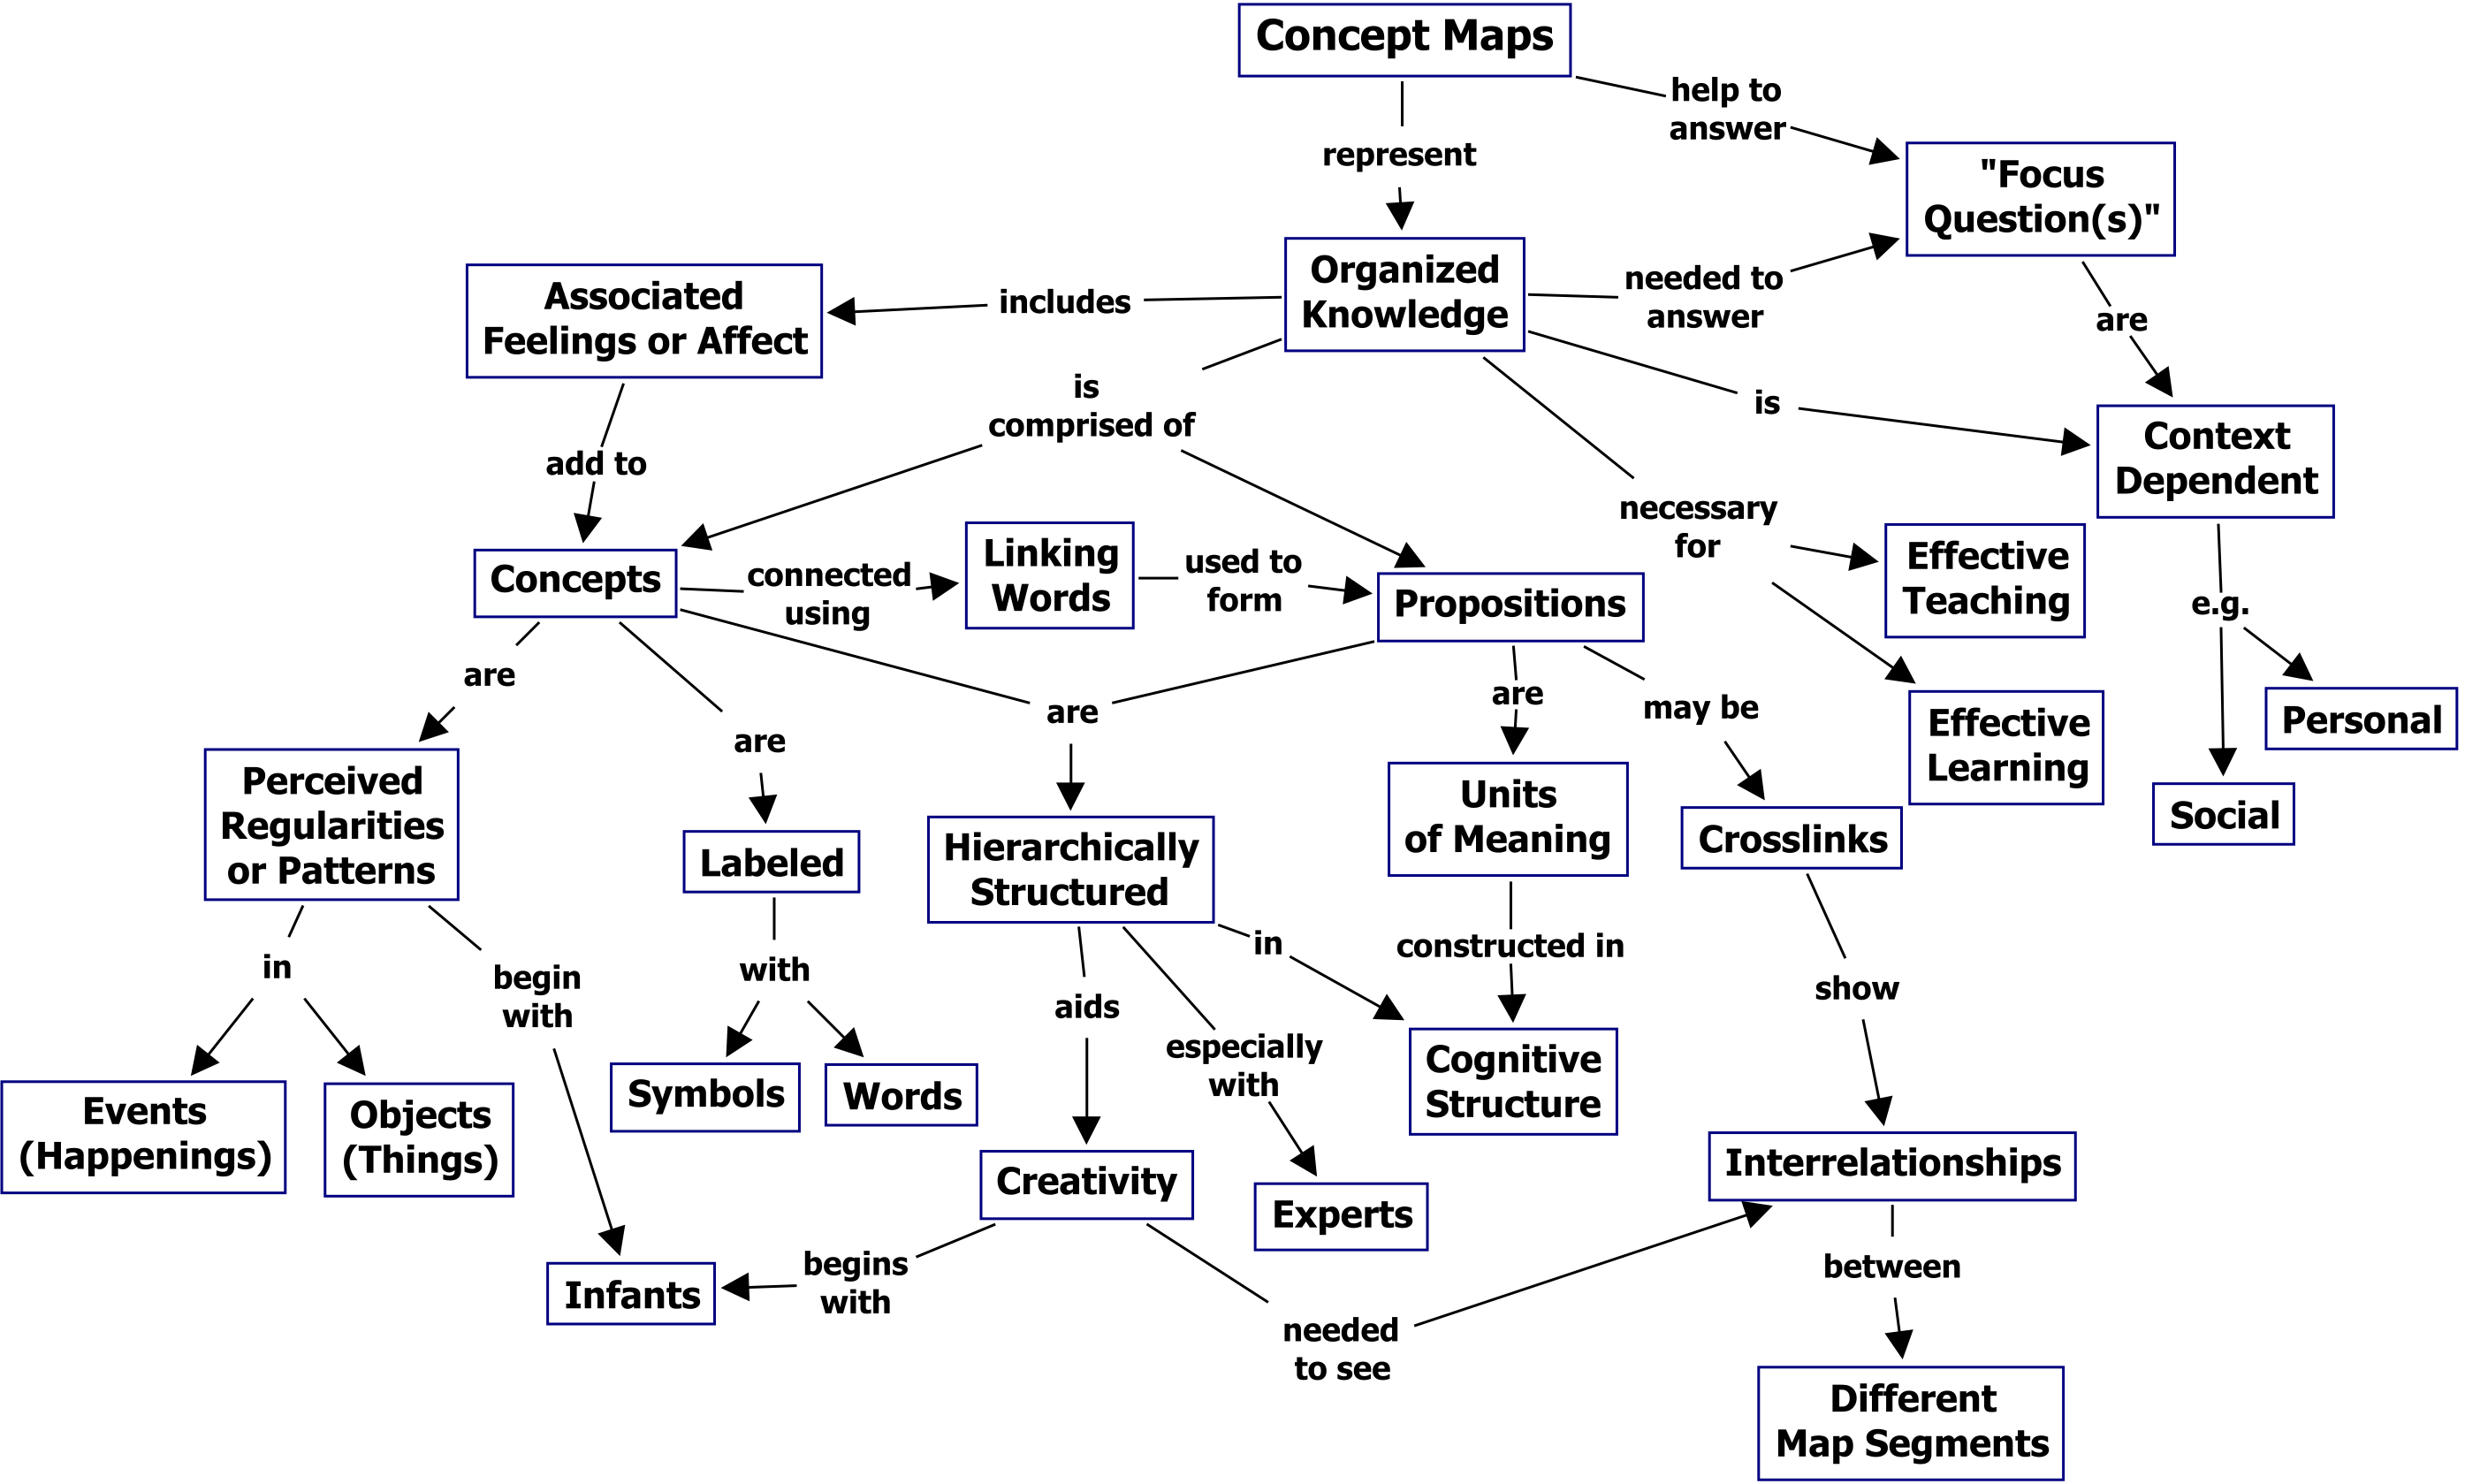
\includegraphics[width=\textwidth]{img/conceptmap}
    \caption{An example of a concept map}
    \label{fig:conceptmap}
\end{figure}

%introduction flashmaps

%n1.2.6.8 and n1.2.6.9 (Counterarguments), n1.2.5, n1.2.10
Therefore, another solution might be the development of a new tool, namely the flashmap system. The intention behind the flashmap system is to combine the paired associate mechanism of the flashcard system with the visual representation of the concept map, and is a new tool designed and developed for this research project. This tool might have the potential to bridge the gap between the two systems and therefore make meaningful and effective rote memorisation possible, for it makes the relations between the concepts explicit to the student.

For evaluating this flashmap system, a group of Dutch highschool teachers of the Stedelijk Lyceum has been found willing to participate, with their students using either the flashmap or the flashcard system for self study parallell with classroom instruction. The content of the instruction will be the history of Dutch literature during the sixteenth and seventeenth century. For example, the students have to learn what the influence is of the Dutch War of Independence on the \emph{Spaanschen Brabander} by Bredero. Because of the content existing mainly of concepts with meaningful relations it fits to the concept map technique and thereby the flashmap system could be significantly beneficial over the flashcard system.

%SUMMARISE, END WITH RESEARCH GOALS

In conlusion, flashcards systems are an effective tool for meaningful learning, but could be enhanced by visualising it with concept maps, and therefore the effects of using a flashmap system over using a flashcard system will be investigated. 

\section{Theoretical Conceptual Framework}

%Describe theoretical framework where you introduce the most important concepts in your study and their relation

\subsection{Flashcards systems}

%n1.1.6, n1.1.1.8.6.1, n1.1.1.3.8.2
There are many different flashcard systems, varying in scheduling algorithms \cite{microlearning}, and offline or online applications \cite{nakata}. The simplest and earliest example is a deck of physical cards, with on one side a question and on the other side the answer to that question. Every day, the student has to go through the deck trying to answer the question on the card. After answering it, the student turns around the card to check whether was correct. If the answer was correct the card goes to the deck for the next day, and if incorrect the card goes to the bottom of the current day's deck.

The main disadvantage of this system is that it becomes time-intensive when more flashcards are introduced, because the student has to go through all of the cards every day. Because of this, newer systems relying on spaced repetition were introduced, with which the time intervals between repetitions increase every time the student answers correctly. \citeA{microlearning} describes three different types of spaced algorithms, namely progressive, responsive, and adaptive. Within progressive algorithms, the rescheduling of cards are always increasing. Responsive algorithms reset the time interval of a card every time the student makes a mistake. Finally, adaptive systems vary the base increase value of the time interval in order to raise success rates towards a given percentage, meaning that the chance of answering the card correctly is estimated to be equal to that percentage. It was found that the last strategy was more effective and more satisfactory to the user than the other strategies \cite{microlearning}.

Furthermore, the transition from physical to digital flashcards is worthwile to consider. The previously described algorithms can more efficiently be conducted by a computer, since it is able to keep track of a learner's performance and control the sequence of items which can be cumbersome if done manually \cite{nakata}. Furthermore, many students have smartphones with them most of the time, and are more convenient than stacks of traditional flashcards \cite{nakata}. The ownly downside to using digital flashcards is that they are less frequently used than traditional flashcards \cite{burgess}. Reasons for this are technical issues, simply forgetting about it, distraction by entertainment apps and preference for traditional flashcards.

The effects of flashcards have mainly been attributed to the spacing effect \cite{nakata, microlearning}, which means that repeated items are better remembered when both occurrences are separated by other events or items than when they are presented in immediate succession \cite{verkoeijen, logan, siegel, xue, karpicke2}.

\subsection{Concept maps}

%n1.2.4, n1.2.8
According to \citeA{eppler}, a concept map is a hierarchical graph showing the relationships between concepts, including cross connections among concepts and their manifestations. The edges contain labels describing the relation between the concepts. They compare the concept map to several different other visual mapping techniques, which are the mind map, the conceptual diagram and the visual metaphor. A mind map is multicoloured and image-centred, is radial and represents semantic or other connections between portions of learned material hierarchically. The benefit of constructing a mind map is that it has a higher memorability than a concept map, but is more difficult to understand by others \cite{eppler}. The conceptual diagram entails abstract concepts in pre-defined category boxes with specified relationships, typically based on a theory or model. This diagram is more suitablefor analysing topics or situations through a proven analytic framework, however they have only a medium memorability and medium understandability by others. Finally, a visual metaphor is a praphic structure using the shape and elements of a familiar artiefact, activity, or story to organise content meaningfully and use the associations with the metaphor to convey additional meaning about the content. This technique is the most meaningful, memorable and understandable in comparison to the other technique, however it has a very limited extensibility \cite{eppler}.

%1.2.6
%\citeA{canas} describes several conditions for using concept maps in learning: no conditions, focus question, root concept, list of concepts, restricting list of concepts, expert skeleton concept maps, concept mapping games, fill-in-the-Cmap and memorise the concept map. These concitions range from low to high scaffolding respectively. The no conditions condition asks students to create a concept map without any scaffolding. This often results in a descriptive instead of an explanatory map, and users are often intimidated and have difficulty constructing a concept map. A focus question helps student to create a more explanatory map by trying to answer specific questions. This has a positive effect on the quality of the resulting maps. A root concept provides the students with a minimum concept map containing the main topics, having a stronger effect than the focus question. The list of concepts condition entails that students get a list of concepts they can use for the construction of their map, resulting in better maps than under no conditions or when provided with a text including the topics. The restrincting list of concepts entails that the students are only allowed to use concepts from the list, which is an effective way of determining the student's prior knowledge. The expert skeleton map restricts the freedom of content and sturture, and overcomes the difficulty of students when getting started. Within coyncept mapping games students are iteratively provided with two concepts and are asked to label the links between them, this has proven to be both effective and affective. Filling in the cmap means that the students are provided with a concept map containing empty nodes which they have to fill in themselves. This technique is not recommended, because this is meant for rote learning purposes and not for meaningful learning. Finally, Memorising the concept map is not recommended for its lack of meaningful learning and integration with other relevant knowledge. It also undermines the need for learners to be actively engaged in assimilating new concepts and propositions into their cognitive structures.

\subsection{Flashmaps}

The flashmap is intended as an integration between the flashcard system and the concept map. The system uses a predefined concept map constructed by an expert which the users have to rote memorise. Concept maps are chosen here, because it has the best combination of understandability and extensibility, and the memorability is facilitated by the flashcard system already. Where a flashcard system would then show a question, the flashmap shows a part of this concept map, where one or more nodes are empty. The user has to think of which concepts would fit in these nodes, and when requesting the answer the flashmaps shows the actual nodes. The student then can indicate per node whether he had it right or not, and they will be rescheduled for review according to the adaptive scheduling algorithm (see figure~\ref{fig:flashmap}). \citeA{canas} describes that fill-in-the-cmap or memorise the concept map conditions are not recommended, because of the information in memorised concept maps not being integrated with other relevant knowledge and the lack of learners being actively engaged in assimilating new concepts and propositions into their cognitive structures. However, they do not provide statistics or literature in order to support this claim, and furthermore the findings from \citeA{karpicke2} about paired associate learning being more effective for meaningful learning than concept mapping also puts this claim into doubt.

\begin{figure}
    \centering
    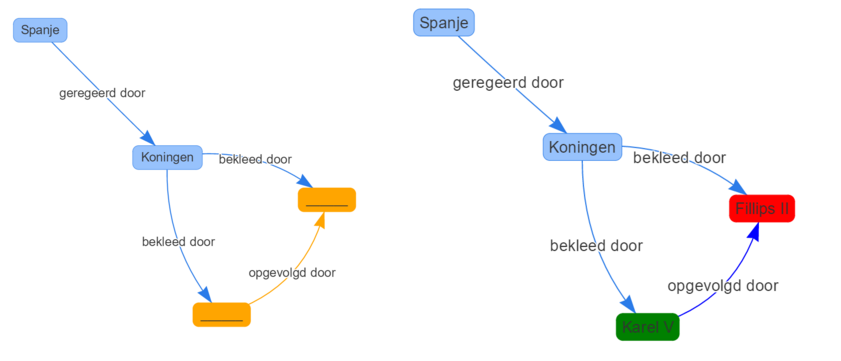
\includegraphics[width=\textwidth]{img/flashmap}
    \caption{A display of the flashmap system, where the user has to think of the concepts fitting in the orange nodes on the left, and has to indicate which nodes were correct on the right}
    \label{fig:flashmap}
\end{figure}

Finally, the flashmap creates the opportunity for a more interactive concept map that starts with a parsimonious and theme-oriented structure which gradually expand the details along with the instruction, which is hypothesisesd by \citeA{tzeng} to mitigate map shock. This phenomenon occurs when users view the kind of larger concept maps that might more fully capture textbook knowledge structures, but is a type of cognitive overload that prevents students from effectively processing the concept map and thereby inhibiting their ability to learn from it \cite{moore}. This mitigation will be facilitated by scheduling the central concepts towards the beginning and the details towards the end.

\section{Research Question and Model}
\newcounter{researchquestion}
\renewcommand{\theresearchquestion}{\Roman{researchquestion}}
\newcounter{subquestion}[researchquestion]
\renewcommand{\thesubquestion}{\alph{subquestion}}


%The research questions (hypotheses if applicable) and model are described here. A figure on your research model is optional.

For researching the effects of the flashmap system relative to the effects of the flashcard system, it is important to consider two main factors: its actual benefits (research question~\ref{benefits}\ref{effectiveness} and~\ref{efficiency}), and its perceived benefits (research question~\ref{perception}\ref{usefulness} and~\ref{ease}). Furthermore, for the validity of the system and of the experiment it is important to investigate how the system was used by the students (research question~\ref{howused}).

To research whether the flashmap system is more effective or efficient than the flashcard system, the learning gain of high school the students will be measured, referring to the knowledge obtained by a student over the course of an instruction. Sequentially, the efficiency of the system is determined by the learning gain controlled for time spend on the system.

For measuring the affectiveness of the systems, the Technology Acceptance Model by \citeA{tam} will be used (see figure~\ref{fig:tam}). This model predicts the use of an information system by measuring the Perceived Usefulness and the Perceived Ease of Use of the user. These variables are mediators between External Variables and Attitude toward using, leading to Behavioural intention to use, which in turn leads to the Actual system use.

\begin{figure}
    \centering
    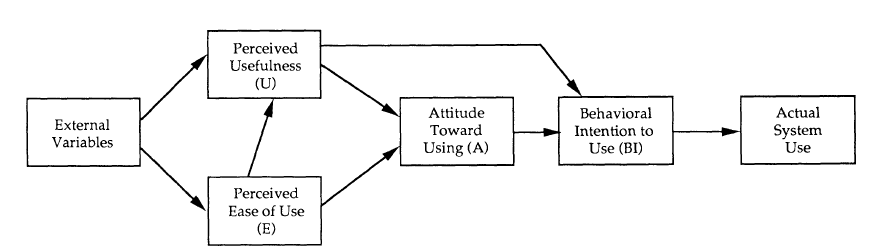
\includegraphics[width=\textwidth]{img/tam}
    \caption{The Technology Acceptance Model by \protect\citeA{tam}}
    \label{fig:tam}
\end{figure}

This leads to the following research questions: Regarding highschool students learning for Dutch literature using the flashmap system in comparison to them using the flashcard system...

\refstepcounter{researchquestion}\label{benefits}
\refstepcounter{subquestion}\label{effectiveness}
\Roman{researchquestion}\alph{subquestion}. ...is the learning gain larger?

\refstepcounter{subquestion}\label{efficiency}
\Roman{researchquestion}\alph{subquestion}. ...is the learning gain larger controlled for the time spend with the system?

\refstepcounter{researchquestion}\label{perception}
\refstepcounter{subquestion}\label{usefulness}
\Roman{researchquestion}\alph{subquestion}. ...do they perceive the system to be more useful?

\refstepcounter{subquestion}\label{ease}
\Roman{researchquestion}\alph{subquestion}. ...do they perceive the system to be easier to use?

\refstepcounter{researchquestion}\label{howused}
\Roman{researchquestion} How did the students use the flashmap or flashcard system?

\section{Scientific and Practical Relevance}

%Describe the expected contribution of your study (how can scientists, practitioners benefit)
Answering the research questions has both practical and scientific relevance. From a practical perspective, it has potential to overcome the criticism from various authors about flashcard systems and answer the need for meaningful rote memorisation. It could furthermore creates new perspectives on the human mind, paving the way for the design of new educational activities based on consideration of retrieval processes \cite{karpicke2}. From a scientific perspective, it could confirm the hypothesis by \citeA{tzeng} that an expanding concept map might mitigate map schock. It also makes way for new research opportunities, for example what the effect is of integrating the flashmap with the games condition formulated by \citeA{canas}. Finally, insights could be gained into how digital flashcard systems might be improved for increased use by students.

%n1.1.3.1
%n2.1


\chapter{Research Design and Methods}

\section{Research design}

%What kind of research is this? (e.g. exploratory, confirmatory, intervention-based, evaluationbased, design-based, etc.). Justify the type of research design(s) you intend to use :descriptive (e.g., case study) ;correlational (longitudinal) ; (quasi-)experimental; review etc.

Research questions \ref{benefit}\ref{effectiveness}, \ref{efficiency}, \ref{perception}\ref{usefulness} and \ref{ease} will be investigated using intervention-based research. Because of the systems being used for self-study by the students, they can be individually assigned to a condition, and this enables the use of a true experimental design. Since this will provide the most valid and reliable results, this research design is implemented in this experiment.

Furthermore, research question~\ref{howused} is a qualitative research question, and therefore an interview will take place after the experiment in order to investigate how the students used the system. Next to the interviews, user data and actions will be logged by the server.

The quantitative and qualitative results will be mixed for the purposes of triangulation and expansion as described by \citeA{mixedmethods}. The interviews and logs could provide insight in the degree of which the systems were used the intended way and in why students had certain perceptions on using the systems. Both triangulation and expansion will be on a partial level of mixing, will take place concurrently, and the quantitative data will be dominant, since the qualitative data exists only to triangulate and expand the quantitative data. 

\section{Respondents}

%This section is where you describe the who will be approached to participate in your study and how many. Explain how they will be selected (sampling method). Make sure this justification fits your research design and questions.

%1.5.4

100 15 to 17 year old tenth grade Dutch high school students will be approached. They already have to prepare themselves for an exam on the same topic and thereby have incentive to learn. To increase the response rate, the students will be rewarded with a \euro{} 5 voucher for participation. The participants will be assigned to either the flashcard or the flashmap condition at random.

\section{Instrumentation}

%Describe the instruments you will use; make a link between the research variables and the instruments explicit (operationalization process) and describe their measurement level if applicable. If you are using existing instruments, provide references.

%n1.5.6

The learning gain will be measured by the means of a pre- and post-test. Both tests will consist of random items from an item bank measuring both knowledge and comprehension levels of the students \cite{bloom}. The tests will be directly based on the concept map, and also will be evaluated by the teacher in order to increase its validity. By using an item bank, the tests will be comparable and thereby the learning gain can be determined by subtracting the score on the pre-test from that on the post-test. Finally, the controlled learning gain is calculated by dividing the learning gain by time spent on the software. The survey will be an adaptation of the standardised Technology Acceptance Model questionnaire \citeA{tamq}.

The interviews will be conducted using a topic list \cite{baarda}, including “frequency”, “usefulness”, “ease of use”, “external conditions”, and “attitudes”, based on the Technology Acceptance Model. The server logs will contain information about the reaction times, the correct responses, the nodes studied, the time investment, the IP address, and the client, which will be registered per user and per session.

\section{Procedure}

%Describe the procedure for your data collection; what will respondents in your study do? Here you can also address any constraints you may need to cope with in the research and the actions to guard its quality and validity. Potential ethical concerns can be addressed here too.

%n1.6

An outline of the procedure is given in figure~\ref{fig:procedure}.

Before the experiment takes place the experiment will have to be approved by the ethics committee from the University of Twente. On approval, the students and their parents will be briefed by means of a letter, which consists out of a general description, conditions (voluntary participation and withdrawal at all times), and rewards. They will also both be asked to fill in an informed consent form.

After that, the students with consent will be provided with a general introduction on flashcards by both the teacher and the researcher within the classroom. Then, when the students log into the system for the first time, the server assigns them randomly to either the flashcard or the flashmap condition. By making the introduction ambiguous enough, the students will not be able to recognise this condition in order to guarantee a double-blind experiment.

Before they start using the system they will be asked for general descriptive information such as date of birth and gender. A code will be assigned to them making it only able for the teacher to determine their identity. After that the pre-test follows, and for the next week will use the system daily for fifteen minutes. Finally the post-test and survey will be conducted. At the end of the post-test, the students can also indicate whether they are willing to participate in the interview.

\begin{figure}
    \centering
    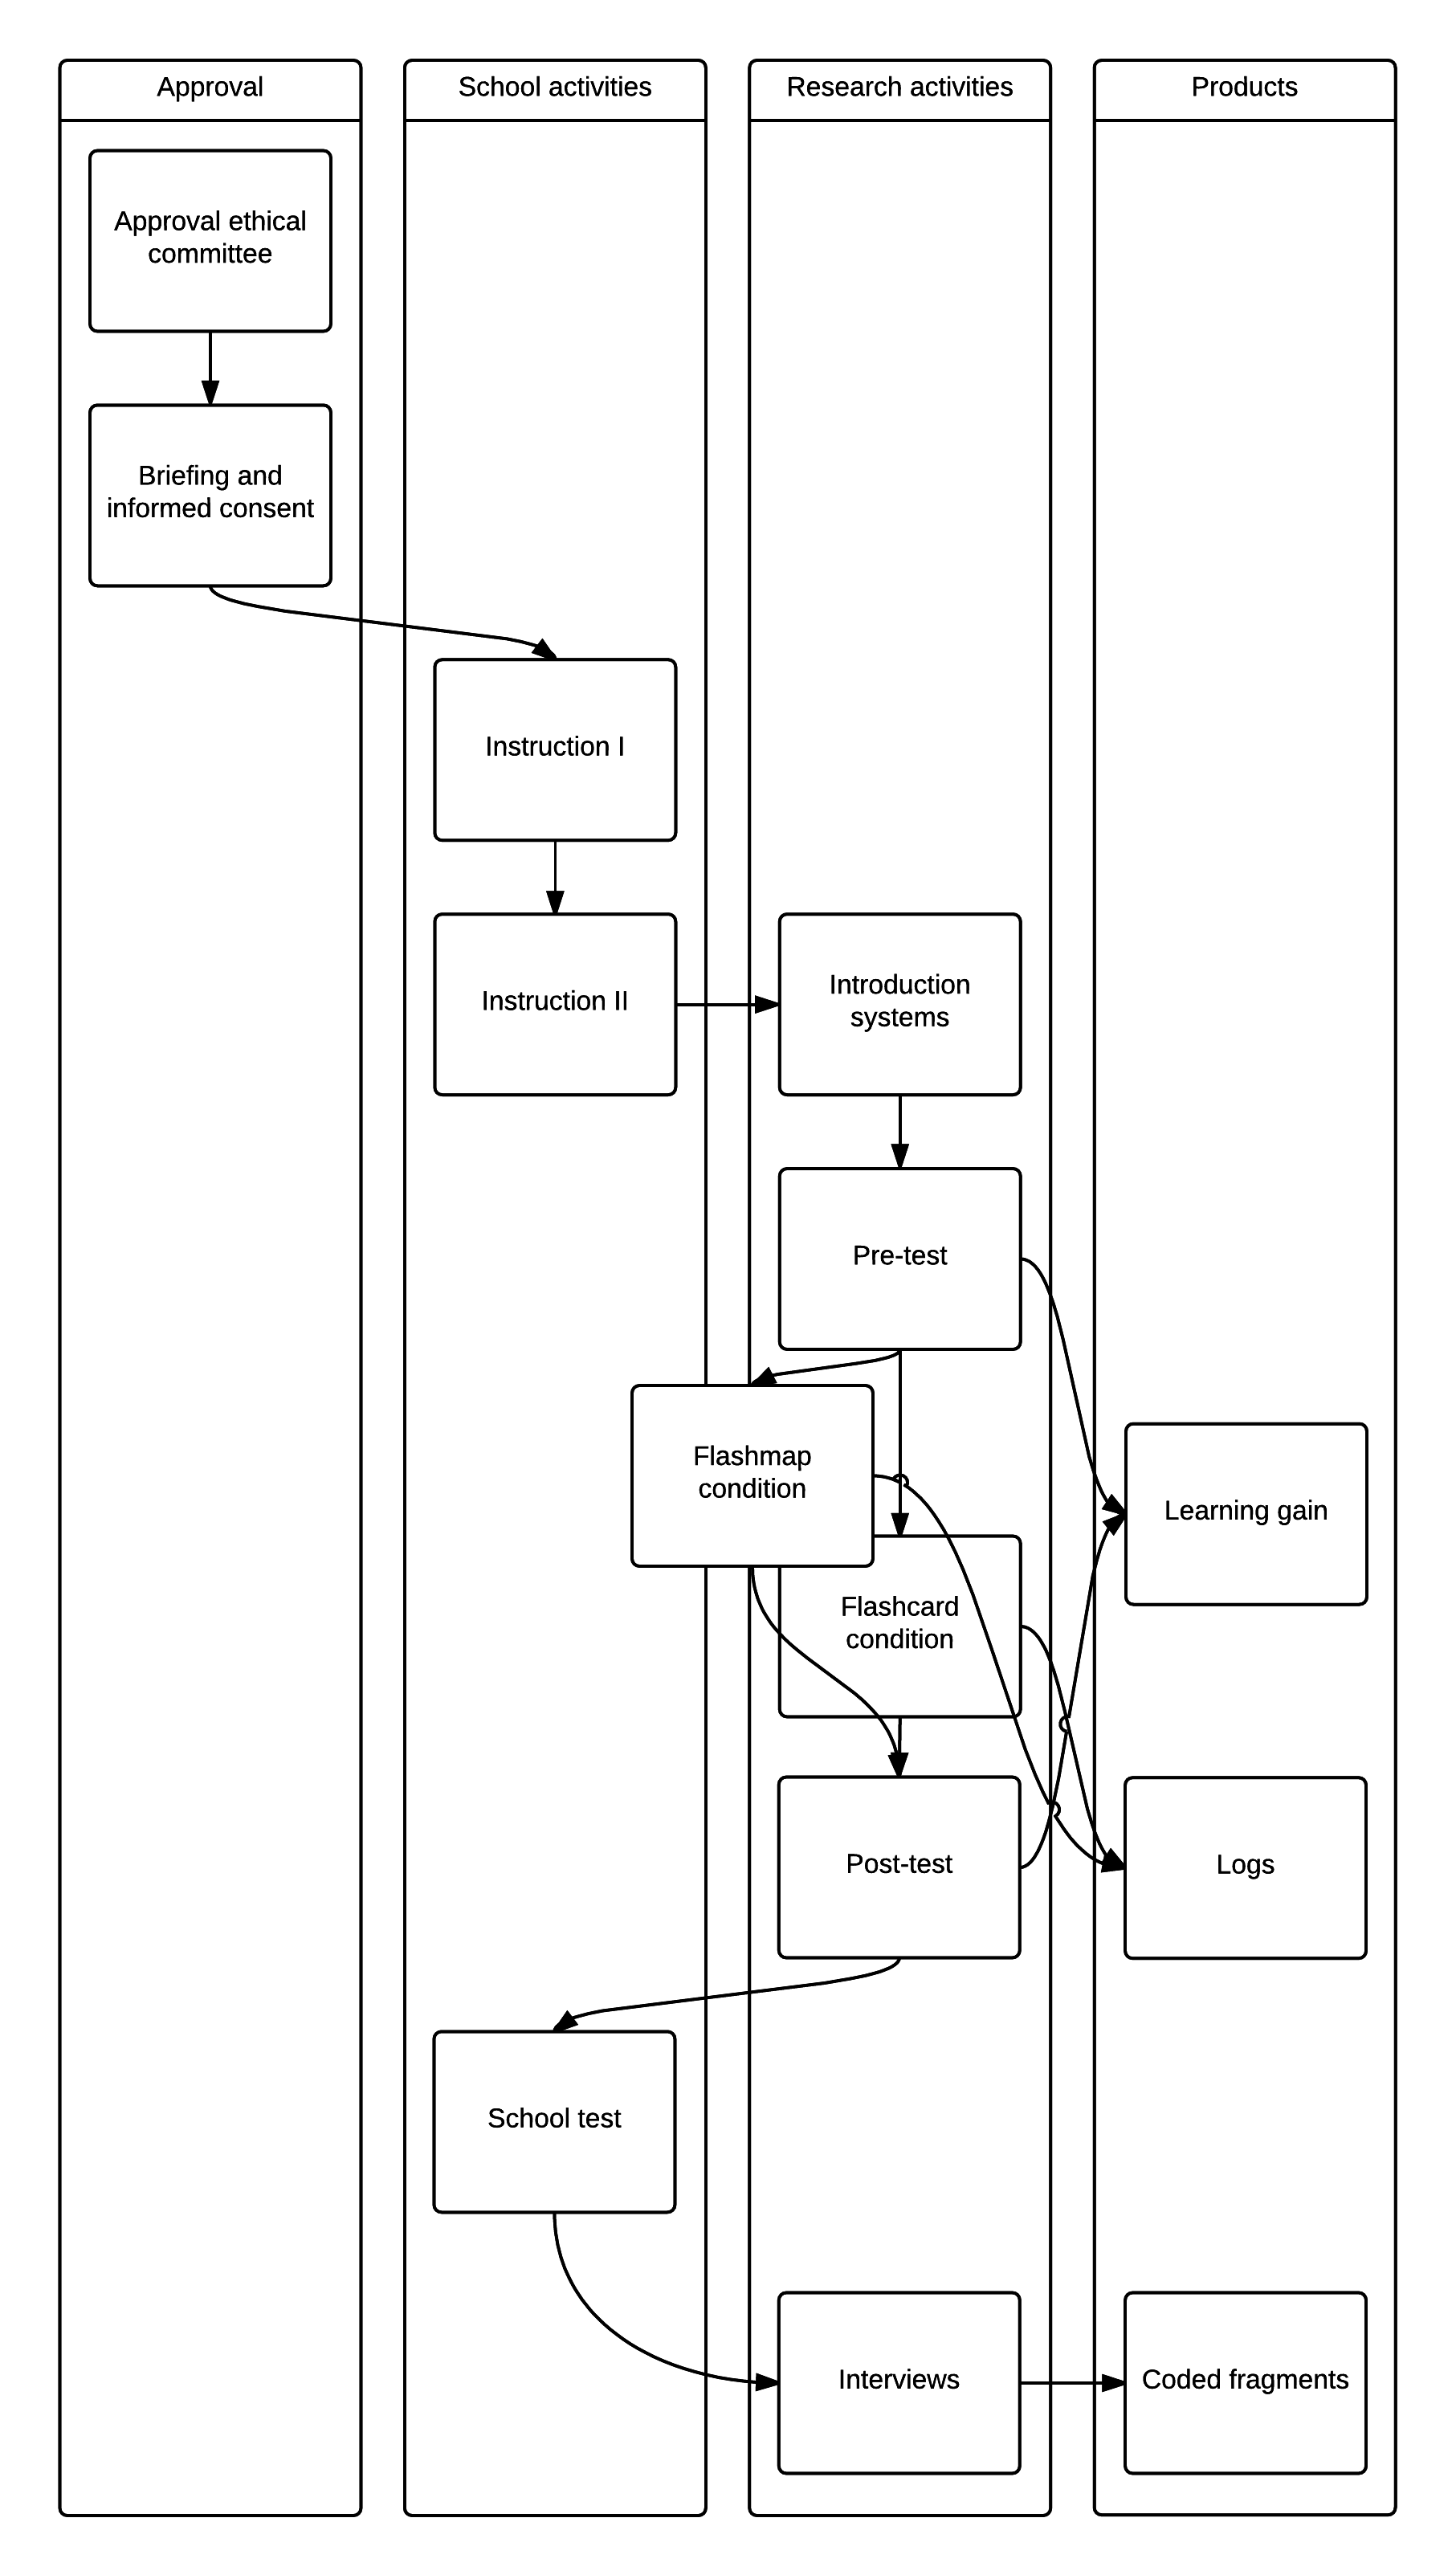
\includegraphics[height=.85\textheight]{img/procedure}
    \caption{An overview of the different steps conducted within the research procedure}
    \label{fig:procedure}
\end{figure}

\section{Data Analysis}

%Describe the type of data you will generate (qualitative, quantitative, mixed-method) and the methods you intend to use to analyze your data. Make sure this fits with your research design and questions. Here you may also address reliability checks for your instrumentation.

Research questions~\ref{benefit}\ref{effectiveness}, \ref{efficiency}, \ref{perception}\ref{usefulness}, and \ref{ease} will be assessed by means of a t-test, using the following hypotheses: 

\begin{tabular}{l l l}
\ref{benefit}\ref{effectiveness} & H0: & $LG_{fc} \leq LG_{fm}$ \\
                                 & Ha: & $LG_{fc} < LG_{fm}$ \\
\ref{benefit}\ref{efficiency}    & H0: & $LGC(fg) \leq LG_{fm}$ \\
                                 & Ha: & $ LGC_{fc} < LG_{fm}$ \\
\ref{perception}\ref{usefulness} & H0: & $U_{fc} \leq U_{fm}$ \\
                                 & Ha: & $U_{fc} < U_{fm}$ \\
\ref{perception}\ref{ease}       & H0: & $E_{fc} \leq E_{fm}$ \\
                                 & Ha: & $E_{fc} < E_{fm}$ \\
\end{tabular}

\noindent where LG = learning gain, LGC = controlled learning gain, U = perceived usefulness, E = perceived ease of use, fc = flashcard condition and fm = flashmap condition. For determining the learning gain, the pre- and post-test have to be scored with a predetermined rubric. The answers will be scored without the scorer being aware whether the question was asked within the pre- or the post-test, or which participant filled in the answer. After both the teacher and the researcher have scored a sample of the answers, the inter-rater reliability will be calculated. The rest of the answers will be scored by the researcher only, and after scoring all of the items the reliability of test items will be assessed further using Item Response Theory \cite{irt}.

The interviews will be transcribed and coded according to \citeA{baarda}, and another inter-rater reliability will be determined by a sample of the interviews coded by the researcher and a peer researcher. The coded fragments will be checked to validate the results from the t-tests, together with the server logs made during the experiment.



\chapter{Planning}

\section{Timeline}

%Include an overview for whole project

\section{Outputs}

%Include descriptions and target dates for final outputs (e.g., advice reports, delivery of products, scientific article) as well as those along the way (e.g. literature review; instruments; data collection).



%\bibliography{references}

\input{./preface/acknowledgements.tex} %Not started
\input{./preface/preamble.tex} %Not started
\chapter{Abstract}

Modern day society requires students to memorise and understand a large number of facts. Currently, a powerful learning tool for comprehension is concept mapping, which refers to drawing meaningful relations between concepts in an associative network. For rote memorisation, flashcard systems are widely employed, which entails students going repeatedly through a set of questions and recalling their answers from memory. Critics have found concept mapping not entailing any method for retaining facts in memory, where others found flashcard learning extracting all meaning and context from the learning process. Therefore, a new learning tool is developed within this study, aiming to bridge the gap between aforementioned learning tools by integrating the visualisation of concept maps within the retrieval mechanism of flashcard learning. The new tool is an augmentation on the flashcard system, which asks the students to fill in empty concepts within given concept maps instead of to answer provided questions. Since retrieval practices --- such as flashcard learning --- have already been found to provide more meaningful learning than concept mapping in a recent study, the new tool is compared with a generic flashcard system for knowledge retention and comprehension. Furthermore, the usefulness and ease of use perceived by the participants are compared. Because of a low response rate, the results from the comparisons are only indicatory for further research. These results include the users of the new tools having a higher learning gain on knowledge retention questions than the flashcard users, and there being no significant difference in increased comprehension, perceived usefulness, and perceived ease of use of the systems.
 %Not started

\part{Introduction}
    \chapter{Project Description}

\label{ch:problem}

Over the centuries, knowledge has been fundamental to any learning process. Socrates already stated that knowledge is the only true virtue, and the tragedian Aeschylus regarded memory as the mother of all knowledge. Moreover, it was not only regarded as important by ancient thinkers, but is still regarded as such by modern scholars on education. Both the taxonomy of learning by \citeA{bloom} as a revision of this taxonomy by \citeA{krathwohl}, as well as the three stages of skill acquisition by \citeA{skillacquisition}, propose that all learning should start with memorising factual knowledge. Furthermore, \citeA{glaserfield}, one of the main founders for critical constructivism, expresses a need for training students so that they permanently possess facts and are able to repeat them flawlessly whenever they are needed, while also understanding what is placed into their memory. \citeA{ltwm} adds to this by stating that in order to perform complex tasks, people must maintain access to large amounts of information, and that solely encoding knowledge is not sufficient. Despite all of this, \citeA{karpicke4} argues that ``[r]etrieval processes, the processes involved in using available cues to actively reconstruct knowledge, have received less attention'' (p. 158), whereas basic research on learning and memory has emphasised that retrieval must be considered in any analysis of learning.

Traditionally, when students have to gain complex and meaningful knowledge -- for example knowledge about a historical event or a chapter in a psychology textbook, they are asked to read the relevant chapter from a provided textbook. However, \citeA{learninginstruction} states that many students have difficulty gaining knowledge in this manner. He breaks reading for comprehension down into four separate skills, which are integrating, organising, elaborating, and monitoring. Integrating refers to relating a text to one's prior knowledge, for which evidence exists that rich background knowledge leads to better inferences about the text, and thereby to better comprehension. This need also has been stressed by \citeA{ausubel}, and forms different problems between individual readers having access to different background knowledge. After integration, the reader has to organise the text, so that the important ideas and the relationships among them are identified. This is mainly a problem for less experienced readers, possessing fewer strategies to quickly identify important parts and thereby spending too much time on reading unimportant information. While organising a text, the student also has to make necessary inferences while reading, or has to elaborate, which is quite difficult for readers when not prompted to do so. Finally, students have to monitor their comprehension, which refers to evaluating their understanding of the text and if necessary adjusting the reading strategy. This is again quite difficult for the average reader, however this can be trained.

While intergrating is something more dependent on the curriculum design, organising and elaborating can be facilitated by a technique called concept mapping, and monitoring by so-called flashcard systems. Furthermore, the latter might be helpful for the integration of the next topic with the current. This research aims to develop a new tool combining these learning tools. In this chapter, concept mapping, flashcard systems, and the new learning tool called the flashmap will be explored on a practical level in order to establish their definitions together with a summary of arguments in favour or opposition of using them as tools for studying textual material, while also describing their current applications within education.

\section{Concept mapping}

A Concept map is a learning tool deviced by Joseph Novak in 1970's, based on constructivist theories of learning. It was originally intended for assessing the structure of student conceptions, before and after instruction, in order to map their prior knowledge and compare it to what they learned during the instruction. This expanded on the notions of \citeA{ausubel}, who stated that what the learner already knows is most important, and that this had to be ascertained before teaching. Although the use of concept maps as an assessment tool remains prevalent \cite{canas, chung, hwang2, ruiz1}, over time, students began to use it as a tool to comprehend textual material by organising and elaborating on the included concepts \cite{canas, eppler, hwang2, karpicke2, nesbit}.

\subsection{Definition}

One definition provided by \citeA{burdo} states that "concept maps are hierarchical representations of knowledge. Construction of them involves linking concepts [...] through the use of linking phrases into propositional statements" (p. 335). The concepts are typically nouns or verbs with or without modifying adjectives or adverbs, and linking phrases specify the relationship between two concepts. \citeA{ruiz1} also mention these elements in their own definition, yet \citeA{canas} and \citeA{eppler} include a few extra features, such as the concepts being ordered in hierarchical fashion. They describe two different kinds of links, which are hierarchical links to indicate ranking between the concepts, and crosslinks to indicate relationships between concepts in different segments or domains of the concpt map. The latter would help to see how a concept in one domain of knowledge represented on the map is related to a concept in another part of the knowledge producer, enabling better connections to prior knowledge of the user. According to \citeA{eppler}, concept maps are always top-down and show systematic relationships among sub-concepts relating to one main concept, however \citeA{canas} state that they can also be cyclical as long as the concepts still have a conceptual hierarchy. Finally, most of the above mentioned articles describe the links between concepts to be directed. In conclusion, the definition of concept maps used within this thesis will be:

\begin{definition}
    A concept map refers to a directed graph, in which the nodes consist of concepts, and the edges of -- either hierarchical or cross- -- links labeled with linking phrases, forming several propositional statements about a knowledge domain.
\end{definition}

\noindent An example of a concept map is displayed in figure~\ref{fig:examplemap}.

For this study, the more interesting aspects of concept maps are the use of concept mapping for elaborating, and of demonstrating meaningful relationships between concepts to learners. The first use of the concept map is known as generative use, and the second as supplantive \cite{instructionaldesign}.

\begin{figure}
    \centering
    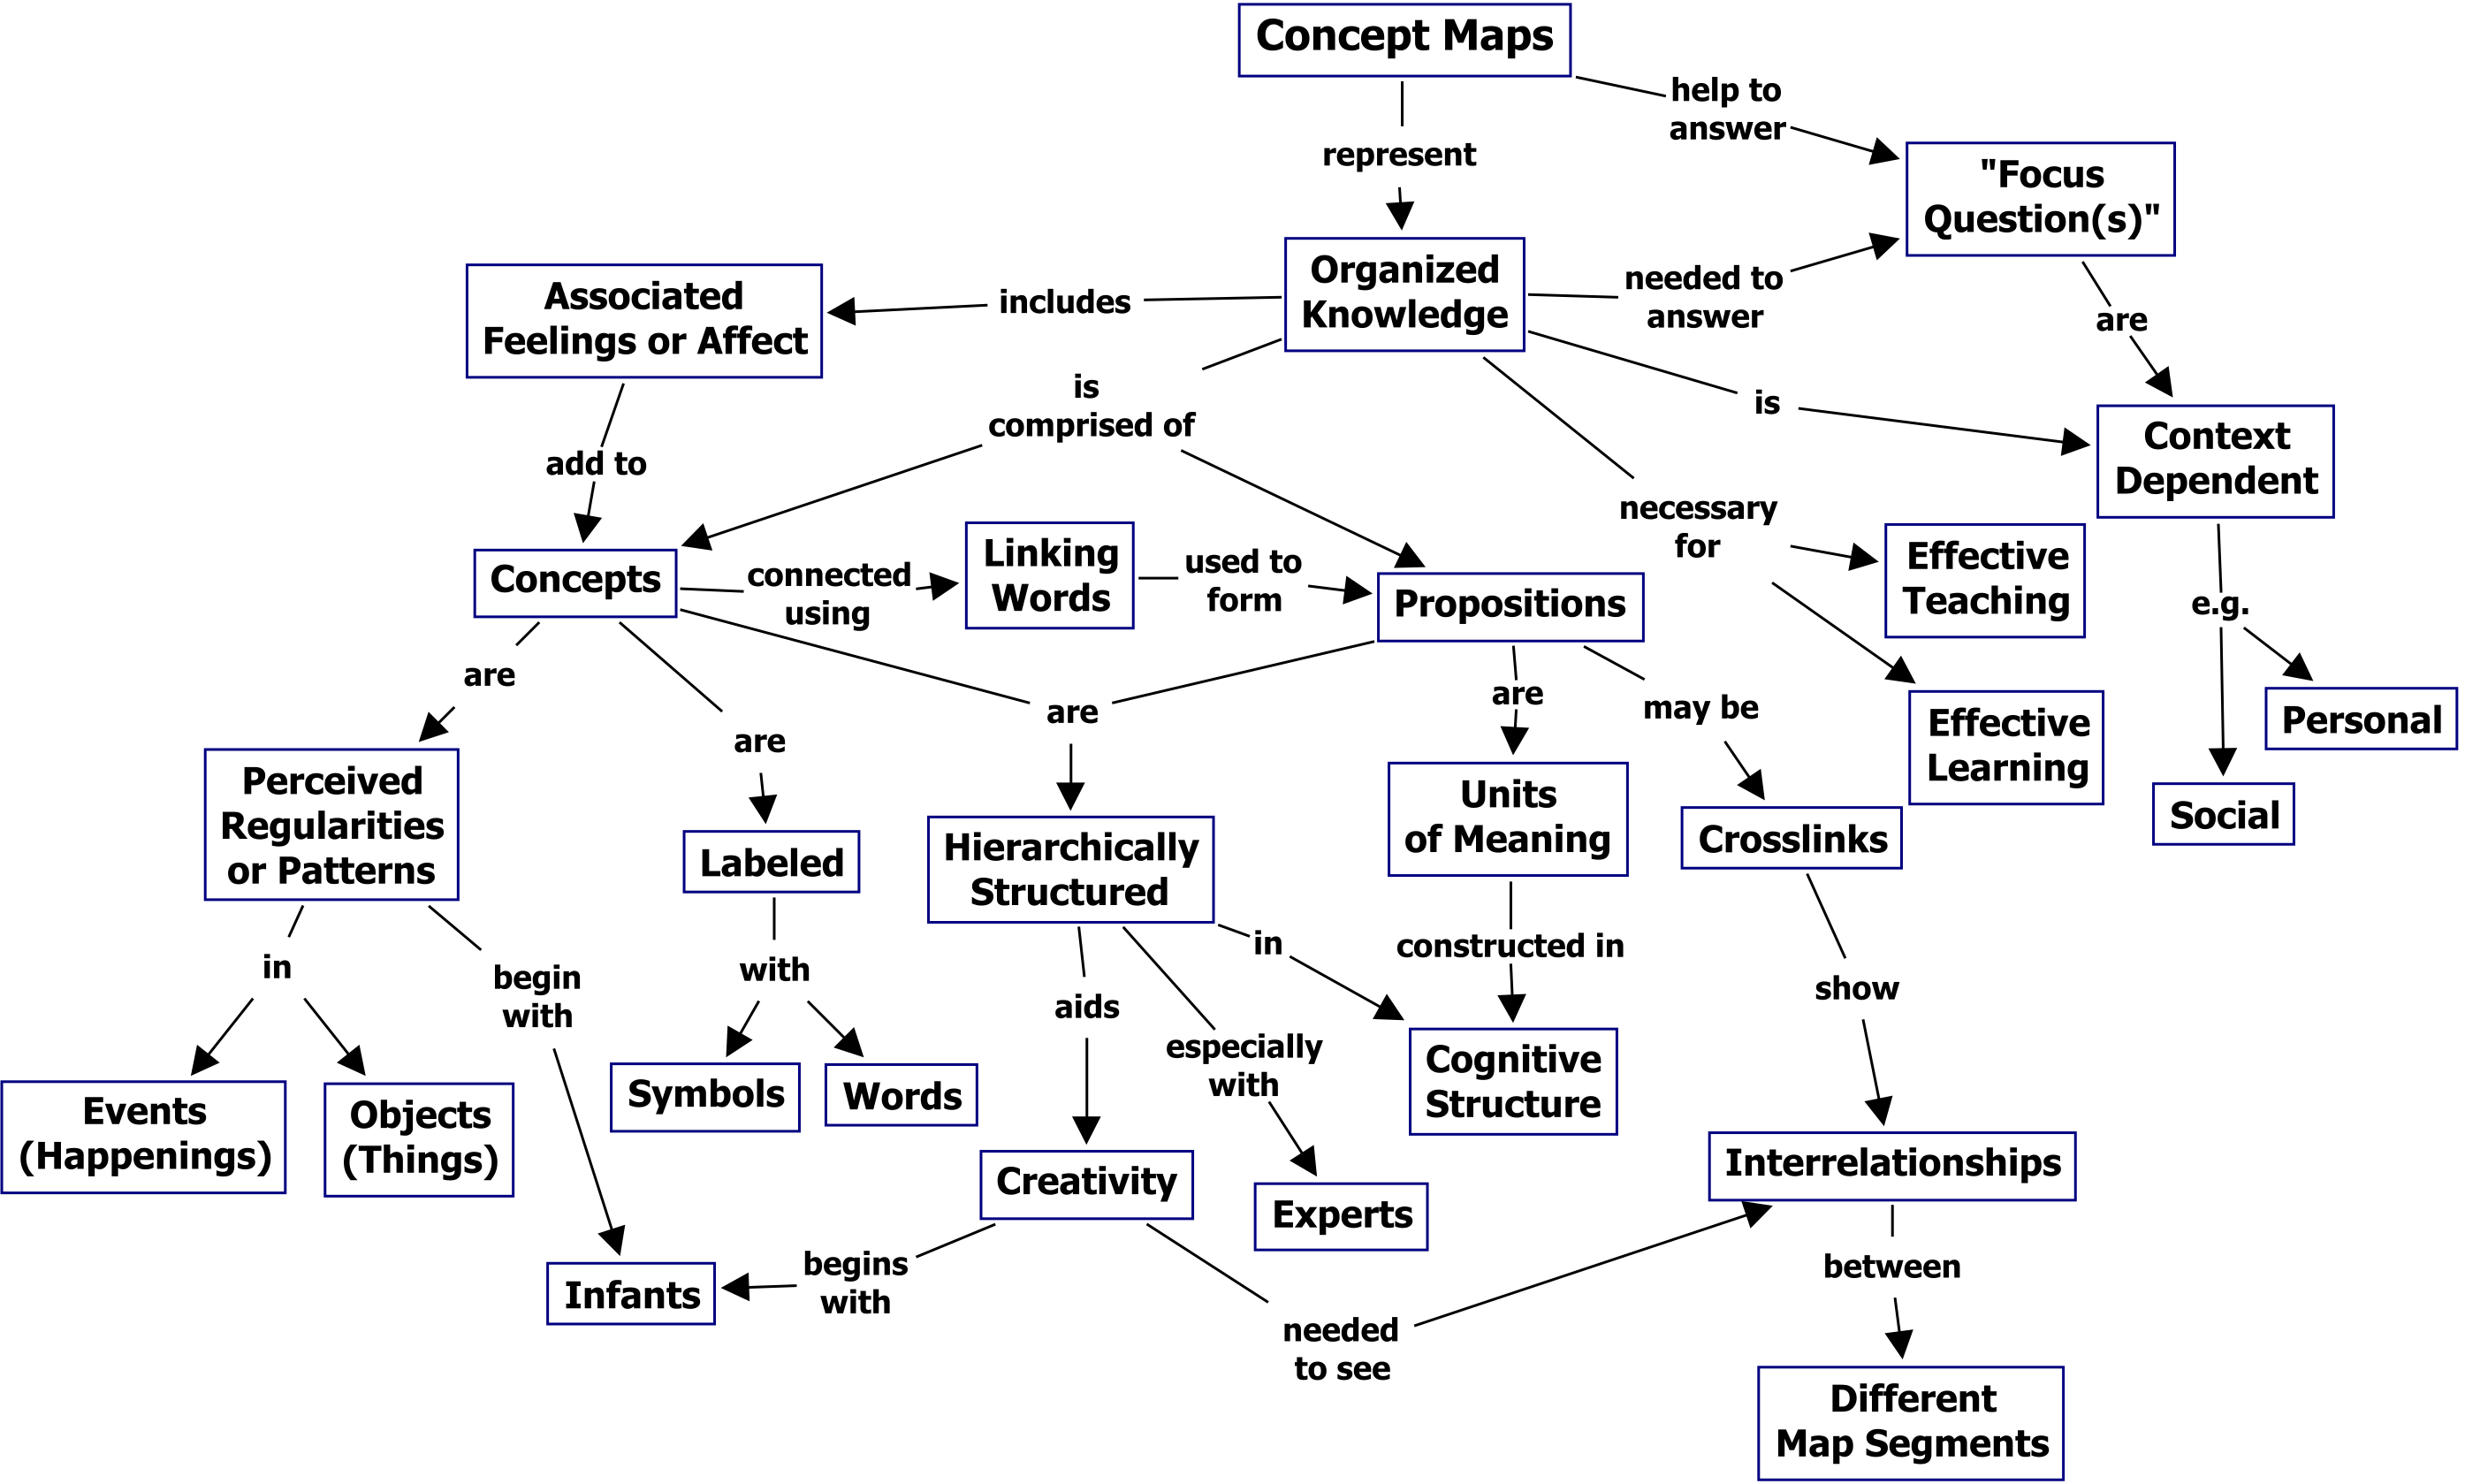
\includegraphics[width=\textwidth]{img/conceptmap.png}
    \caption{A fraction of the concept map used in this study}
    \label{fig:examplemap}
\end{figure}

\subsection{Effectiveness}

Multiple studies, both qualitative and quantitative, have demonstrated that concept maps can promote meaningful learning \cite{canas, hwang2, nesbit, subramaniam}. When comparing the concept mapping strategy with traditional teaching strategies (in a study conducted within the context of tertiary chemistry), \citeA{singh} found that the concept map teaching strategy was more effective, however that it was most effective if both strategies were used in combination. One of the positives of the concept map is that it does not provide learning by means of disconnected facts, but rather as a cohesive narrative placing emphasis on the connections between the concepts. However, most studies state that merely studying a concept map (supplantive use) is not sufficient, and that the activity of constructing the concept map (generative use) is essential for using it as a learning tool. \citeA{canas} even state that meaningful learning does not work by memorising a concept map, because the information is not integrated with other relevant knowledge. Furthermore, \citeA{nesbit} state that much of the benefits may be due to greater learner engagement rather than the properties of the concept map as an information medium. However, no studies were found testing these hypotheses, and yet \citeA{blankenship} have found that expert generated concept maps are believed to help students form conceptual understanding. Still, this study did also indicate that greater maps (more than 20 nodes) used within textbooks lead to \emph{map-shock}: ``a type of cognitive overload that prevents students from effectively processing the concept map, thereby inhibiting their ability to learn from it'' \cite[p.~3]{moore}. Finally, \citeA{eppler} enlists some of the main advantages and disadvantages in comparison to other visualisation formats (mind maps, conceptual diagrams, and visual metaphors). A positive aspect is that students can gain information rapidly, because of the systematic, proven approach to provide an overview and the emphasis on relationships and connections among concepts. On the other hand, the technique of concept mapping is not easy to apply by novices and requires exstensive training, since otherwise the maps tend to turn out to be idiosyncratic. Furthermore, although better understandability is provided, the overall pattern does not necessarily assist memorability. Finally, the quality of concept maps can be assessed through evaluation rules, however this turns out to be quite a time consuming task for the tutors.


\subsection{Applications of concept mapping}

An article by \citeA{desimone} states that despite the effectiveness of concept mapping, its use is not that widespread because students find it cognitively difficult, time consuming, or nonessential vis-\`{a}-vis task demands. The article then provides an overview of how concept maps are generally used in the classroom: as an external scratch pad to represent major ideas and their organisation, as a time-efficient tool for mental construction, and as a tool for exchange of diversifying ideas and gaining new insights; and provides benefits and limitations for each of these uses. When used as an external scratch pad, students map their ideas on paper by writing a main idea and linking it with other related concepts through action words and arrows. Although most students find it helpful to offload information externally and detect and correct gaps and inconsistencies in their knowledge, they still find the process of mapping to be time consuming. This is because they often have to make major revisions, requiring them to redraw the concept map multiple times. Therefore, a more time-efficient approach might be mental concept mapping, where they had to represent answers within the map to questions such as ``what are the key ideas?'' and ``how are these ideas related?''. This provided to be more efficient due to better mastery of the mapping strategies, and thereby more comfortable for the students. Finally, concept mapping enables students to draw relationships more freely, due to its flexibilities regarding layout and adding or removing concepts or relations. It also stimulated collaborative learning by enabling easier sharing and even co-construction. Nonetheless, of these strategies, the traditional strategy remains the most prevalent, since it is the best known use of concept mapping. Finally, as already stated before, \citeA{moore} state that multiple textbook publishers started including concept maps within their textbooks in order to provide an overview of the content.

\section{Flashcard system}

In contrast to concept maps, a flashcard system is not intended for meaningful knowledge encoding, but rather for the rehearsal of knowledge so that it keeps active and as such is prevented from being forgotten.

\subsection{Definition}

In the context of language learning, \citeA{nakata} defines flashcard systems as learning tools in which ``target items are presented outside meaning-focused tasks, and learners are asked to associate the L2 [foreign language] word form with its meaning, usually in the form of a first language translation, L2 synonym, or L2 definition'' (p. 17). This form of learning is also referred to as a \emph{paired-associate format}, which refers to learning by being presented by cues and the learner having to recall an associated counterpart. Besides vocabulary learning, it can also be used to memorise word definitions or topographical information. In order to be more inclusive of other use cases, the following general definition is proposed:

\begin{definition}
    A flashcard system refers to any system in which a learner is presented with cues and has to recall their counterparts from a paired-associate format.
\end{definition}

The most simple form of a flashcard system is a system where the learner has a stack of cards, with each containing a retrieval cue on one side and the correct associated response on the other side. A learning session then consists of going through the whole stack each day and trying to come up with correct answers. Efficiency can then be increased by repeating difficult cards more often, or skipping reviewing certain easy cards for multiple days. This way only on the pairs which are more needy of retrieval are focused on. Finally, the size of the stack of cards can be increased over multiple days in order to improve the spreading of cognitive load. Next to these paper flashcards, there is also a multitude of digital flashcard systems available \cite{hwang2, nakata, microlearning}, which allows for automating the rescheduling of flashcards, providing better access to more advanced algorithms for the rescheduling of flashcards.

\subsection{Effectiveness}

Flashcard systems have not been completely free from criticism by other researchers. \citeA{hulstijn} for example describes flashcards as a relic of the old-fashioned behaviourist learning model, and \citeA{mccullough} states that the main emphasis of flashcards is memorisation, not comprehension. However, \citeA{zirkle} states that it is still important for teachers and students to understand and utilise memory in such a way that a store of knowledge is produced that remains flexibly retrievable in a variety of contexts over a period of time, even more so because even though it is deemed useless to learn without comprehension, students still should learn by heart many conventional facts \cite{glaserfield}. Flashcards have been found to be both a time efficient tool for learning large numbers of facts and an effective tool for these facts to be more resistant to decay in comparison to traditional teaching methods \cite{nakata}. Their effectiveness also has been demonstrated accross studies in different contexts, for example that of language learning \cite{chien, macquarrie, mccullough, nakata}, word recognition \cite{joseph}, psychology courses \cite{burgess, golding}, and geography \cite{zirkle}. Therefore, many authors support pursuing research into flashcards and its effective application into classrooms.

\subsection{Design features}

\citeA{nakata} also describes general design features of flashcard software, which are seperated in terms of creation and editing of flashcards, and learning of flashcards. Examples are whether learners are able to create their own flashcards or flashcard sets, whether learners merely have to recall an answer or have to produce an answer, how big a learning session is and how repetitions are scheduled. Partly, these features are also applicable on paper flashcards. The features will be further elaborated later on page INSERT REFERENCE TO DESIGN CHAPTER, but for now it is sufficient to state that at the time of writing there are no commonly accepted guidelines for how flaschard software should be designed. This mainly is due to the fact that not a lot of research is conducted on specific design-features, because of research reviewing mostly the same program, and there being discrepancies in the way they are designed. Therefore, further research is necessary in order to establish these guidelines.

%TODO: add reference to design chapter

\subsection{Application of flashcards}

\label{subsec:fcapplication}

Multiple sources describe an increase in the use of flashcards in education: \citeA{kornell} states that ``perhaps no memorisation technique is more widely used than flashcards'' (p. 125), and more recently textbooks have also started making them available \cite{burgess, golding}. Two reasons for the popularity of flashcards are provided by \citeA{golding}: students can generate flashcards for themselves, they feel that they are `doing' something when they study. Most of the studies found are based around flashcard usage in language courses \cite{nakata, joseph, chien}, but there also exists a study by \citeA{golding} describing that 70\% of general psychology students used flashcards for at least one exam.

\citeA{chien} and \citeA{nakata} describe that multimedia and digital flashcards are used widely within vocabulary learning, because they can be easily programmed to keep track of performance and better control the sequency, which is cumbersome if done manually. Furthermore, students might be more motivated using digital flashcards because of the enhanced presentation of materials due to their multimedia capabilities. However, \citeA{golding} still found the majority of students using written flashcards. These findings surprised \citeA{burgess}, since many students have their smart phones with them most of the time -- 75\% of students report using smartphones during breaks, meetings etc, 55\% while waiting, and 45\% for school related uses -- and phones are more portable than large stacks of traditional flashcards. However, when he pursued the study by providing students with either written or digital flashcards, students used the digital flashcards less frequently than the traditional flashcards, even when the students had to make their own flashcards. Reasons students provided were technical issues such as battery consumption, simply forgetting about it, using entertainment apps instead of studying, and preference for traditional flashcards.

\section{Comparison of the two tools}

In summary, most studies describe concept mapping as a tool for meaningful encoding, whereas flashcards are described as a tool for rote memorisation, and therefore imply that the former approach leads to more comprehension than the latter. A recent study by \citeA{karpicke2} researched this hypothesis by having participants study a science text with four different learning conditions and prompting them afterwards with verbatim and inference questions and metacognitive predictions. Within the first condition, students only had to read the text and then answer the quesions. The second group studied the text in four consecutive study periods. Students within the third group studied the text in one initial study period and then created a concept map after being instructed in concept mapping. The final group studied the text in an initial study period and then had to recall as much as they could on a free recall test, and repeated this strategy. The time spent on concept mapping and recalling was equal. When analysing the results, it was found that the retrieval practice group performed highest on both the verbatim and the inference questions, whereas the repeated study and concept mapping groups performed about equally well and the study once group performed the worst. Interestingly enough, the retrieval practice group judged their own learning the lowest, and the repeated study group the highest. The same effect of concept mapping and retrieval practice was found again in a second reproduction study, and also in another study by \citeA{burdo}. It is theorised that during elaboration, subjects attain detailed representations of encoded knowledge by linking concepts together in meaningful ways, but that during retrieval, subjects use retrieval cues to reconstruct meaning en thereby already organise the content in a meaningful way. \citeA{karpicke2} conclude that these insights could pave the way for the design of new educational activities with retrieval practices in mind.

\section{Flashmap system}

\label{sec:intro_flashmap}

It can be concluded that both of these tools are helpful for studying, since concept maps help students organise by drawing hierarchical links and elaborate on the content by drawing cross-links, and flashcards help students monitor their understanding of the text and retain the knowledge in order to facilitate integration with a following topic where the knowledge may prove relevant. The object of this study is therefore to create a new learning tool, and intends to combine both the visual overview of concept maps with the retrieval mechanism of flashcard systems by means of a new digital tool, which from this point onwards will be referred to as the Flashmap system. It will present incomplete parts of a concept map, in which the student has to fill in the missing parts of propositions represented by that map (see figure~\ref{fig:flashmap}). These parts will consecutively be repeated according to algorithms already used by digital flashcard systems. The flashmap system might have the potential to bridge the gap between the two systems, and therefore make meaningful and effective rote memorisation possible, for it should make the relations between the concepts explicit to the student, thereby increasing the organisation of the knowledge and reducing the segregation of facts. Hereby, this tool might facilitate the needs stressed by both \citeA{karpicke4} and \citeA{zirkle} of more meaningful retrieval. Furthermore, by having the students memorise the concept map and graduately expanding on it, the generally experienced map shock occuring with expert-generated concept maps might also be mitigated (see also \citeNP{tzeng}).

\begin{figure}
    \centering
    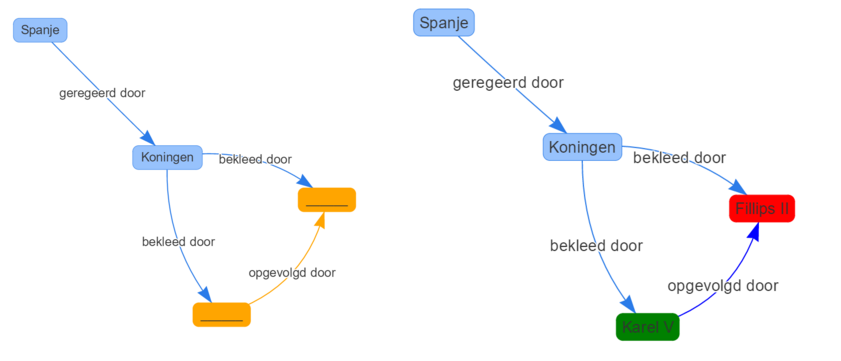
\includegraphics[width=\textwidth]{img/flashmap}
    \caption{A display of the flashmap system, where the user has to think of the concepts fitting in the orange nodes on the left, and has to indicate which nodes were correct on the right}
    \label{fig:flashmap}
\end{figure}

\section{Evaluation}

\label{sec:intro_evaluation}

This project does not only aim to develop a flashmap system, but also to evaluate it by comparing it to a similarly functioning flashcard system. For evaluating this flashmap system, a group of Dutch high school teachers of the Stedelijk Lyceum has been found willing to participate, with their students using either the flashmap or the flashcard system for self study parallel with classroom instruction. The content of the instruction will be the history of Dutch literature during the sixteenth and seventeenth century. For example, the students have to learn what the influence is of the Dutch War of Independence on the \emph{Spaanschen Brabander} by Bredero. Because of the content existing mainly of concepts with meaningful relations it fits to the concept map technique and thereby the flashmap system could be significantly beneficial over the flashcard system.

\newcounter{researchquestion}
\renewcommand{\theresearchquestion}{\Roman{researchquestion}}
\newcounter{subquestion}[researchquestion]
\renewcommand{\thesubquestion}{\alph{subquestion}}

The research aims to investigate the following questions: Regarding high school students learning for Dutch literature using the flashmap system in comparison to them using the flashcard system...

\refstepcounter{researchquestion}\label{benefit}
\refstepcounter{subquestion}\label{effectiveness}
\Roman{researchquestion}\alph{subquestion}. ...is the learning gain larger?

\refstepcounter{subquestion}\label{efficiency}
\Roman{researchquestion}\alph{subquestion}. ...is the learning gain larger controlled for the time spend with the system?

\refstepcounter{researchquestion}\label{perception}
\refstepcounter{subquestion}\label{usefulness}
\Roman{researchquestion}\alph{subquestion}. ...do they perceive the system to be more useful?

\refstepcounter{subquestion}\label{ease}
\Roman{researchquestion}\alph{subquestion}. ...do they perceive the system to be easier to use?

\refstepcounter{researchquestion}\label{howused}
\Roman{researchquestion} How did the students use the flashmap or flashcard system?

For researching the effects of the flashmap system relative to the effects of the flashcard system, it is important to consider two main factors: its actual benefits (research question~\ref{benefit}\ref{effectiveness} and~\ref{efficiency}), and its perceived benefits (research question~\ref{perception}\ref{usefulness} and~\ref{ease}). Furthermore, for the validity of the system and of the experiment it is important to investigate how the system was used by the students (research question~\ref{howused}).

To research whether the flashmap system is more effective or efficient than the flashcard system, the learning gain of high school the students will be measured, referring to the knowledge obtained by a student over the course of an instruction. Sequentially, the efficiency of the system is determined by the learning gain controlled for time spend on the system.

For measuring the affectiveness of the systems, the Technology Acceptance Model by \citeA{tam} will be used (see figure~\ref{fig:tam}). This model predicts the use of an information system by measuring the Perceived Usefulness and the Perceived Ease of Use of the user. These variables are mediators between External Variables and Attitude toward using, leading to Behavioural intention to use, which in turn leads to the Actual system use.

Finally, for the answering the final question an interview will be conducted with a sample of the participants, and by the server logging usage information about the user.

\begin{figure}
    \centering
    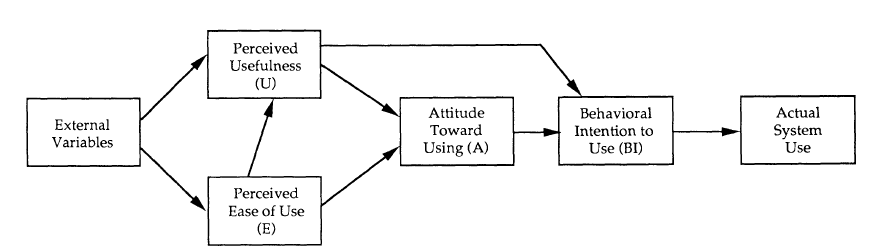
\includegraphics[width=\textwidth]{img/tam}
    \caption{The Technology Acceptance Model by \protect\citeA{tam}}
    \label{fig:tam}
\end{figure}

Answering the research questions has both practical and scientific relevance. From a practical perspective, it has potential to overcome the criticism from various authors about flashcard systems and answer the need for meaningful rote memorisation. From a scientific perspective, it could confirm the hypothesis by \citeA{tzeng} that an expanding concept map might mitigate map shock. It also makes way for new research opportunities, for example what the effect is of integrating the flashmap with the games condition formulated by \citeA{canas}. 

The following chapterwill elaborate further on the cognitive theories underlying concept mapping and flaschard systems on page~\pageref{ch:theory}, after which the design and development of the flashmap will be described in part II. The research conducted within this project and its results will be described in part III, and finally part IV will be elaborating on additional features of the flashmap system and how these could be evaluated by further research.
 %Reviewed by Tobias TODO: missing references to labels
    \chapter{Context}

As can be read in the previous chapter, the aim of this study is to develop and evaluate a tool designed for the purpose of meaningful memorisation. However, why is it actually important to memorise? This question has historically been debated since the days of the early Greek philosophers, and still remains relevant today. Therefore, before delving into the effectivity and specifications of the tool itself, it seems important to briefly reflect on this question first. This chapter does not aim to answer this age-old question, but rather tries to provide both some philosophical and historical context, for better understanding of the relevance of a better memorisation tool, and what `better' generally entails. Furthermore, it more specifically will relate these questions specifically to the tools investigated within this study.

\section{Five educational philosophies}

Curriculum theorisers have proposed many different systems of categories \cite{curriculumtheory}, of which the aim is to investigate which goals people involved with education have, and which aspects they therefore regard as being important. \citeA{educationalphilosophy5} differentiates between the five philosophies of education \emph{Perennialism}, \emph{Essentialism}, \emph{Progressivism}, \emph{Reconstructionalism}, and \emph{Existentionalist education}, which have also (at least partly) been acknowledged by other authors \cite{educationalphilosophy, educationalphilosophy2, educationalphilosophy3, educationalphilosophy4}. Furthermore, \citeA{educationalphilosophy3} have found these categories to be sufficiently valid and reliable upon measuring their prevalence among teachers. Therefore, these categories will be discussed further individually in order to provide philosophical context towards the function of knowledge.

\section{Perennialism}

According to perennialism, there is no alteriar motive for attaining knowledge, but rather that attaining knowledge is a purpose on itself. This is along the words of Socrates, who concluded that knowledge is the only virtue. This he concluded based on that wisdom is the same as knowledge \cite{wisdomknowledge}, that wisdom is one of the five cardinal virtues, and that all other virtues (e.g. justice) are merely derived from the virtue of wisdom.

The perennialists are mainly based on either the general philosophy of idealism or of realism. The most notable idealist perennialist are the scholastics, who focused on teaching the great classical and religious works in order to better understand their supreme being. Realist perennialists believe the classic works still have much implications today, and therefore should be taught to the next generation.

Methods generally practiced by are considered to be rather traditional, example of these are memorisation, reading, writing, drill, and recitation. It is also the only philosophy which has many of its followers believing that education should be directed towards the intellectually gifted, and that other students should only receive vocational education.

Perennialism has been the leading philosophy in academics before the enlightenment. In the classical era, Greek students had to memorise and recite famous poetry, such as the Iliad and Odyssey by Homer, because these were believed to ``provide great moral lessons and taught them what it meant to be a Greek'' \cite[p.139]{searchgreeks}. This academic tradition was then perpetuated throughout the middle ages by the scholastics, who used the rationalism of the Greek philosophers to defend christian doctrine -- most notably in the \emph{Summa Theologica} by Thomas Aquinas. Scholastic instruction consisted of four elements: \emph{lectio}, the reading of an authoritative text; \emph{mediatio}, a reflection on the text; \emph{quaestio}, questions from students about the text; and \emph{disputationes}, a discussion about controversial \emph{quaestiones}. With the coming of the enlightenment, academics transisted from using classical idealism as a source of truth and instead used experimentalism as a source of learning about the material world and verifying truth claims, and humanism as a means to a better understanding of the human endevour. Nonetheless, perennialism remained a prominent philosophy in education until the industrial revolution in the 19th century, and still has a place in modern society in the form of for example the Great Book program proposed by Hutchins, albeit in a far lesser degree than before the enlightenment.

\section{Essentialism}

Essentialism is generally seen as a child philosophy of perennialism, and is more goal oriented than its parent. Its purpose is to pass on knowledge to new generations in order for them to be able to function in society, and focuses on subject matter. It is also a very teacher oriented approach to education.

This philosophy also is based on both idealism and realism, whereas the idealists think the content comes from history, language and the classics, and the realists think it comes from the physical world, including mathematics and the natural sciences.

Just like perennialism, essentialist teaching methods are rather traditional, and include returning to the three R's, reading, lectures, memorisation, repetition, audio-visual materials, and examinations.

The earliest form recognisable as essentialist is the factory model of education \cite{honours}, which was a means to deliver education to the general public for the benefit of the whole society. This model was improved upon by introducing aspects of behaviourism with the introduction of reinforcement and repetition in order to shape the behaviour the teacher wanted. Furthermore, it introduced the audio-lingual method, where the whole class as a group chanted correct answers or key phrases. Furthermore, because of the importance of high-quality instruction, cognitivism contributed towards a better understanding of how to present materials more effectively. Essentialism still remains a popular philosophy in the form of people wanting to go `back to basics' or wanting more order in the classroom.

\section{Progressivism}

Progressivism go one step further than essentialists in a sense that new students should not only be taught to function in society, but to go beyond and improve society. This might seem like a small step, but is rather involved for it has its base in opposing authorianism instead of conforming to it.

It also has its root philosophy in experimentalism, where truth is not constant such as in idealism or realism, but rather is constantly in transition to a better understanding. Therefore, a progressivist curriculum focuses itself not on teaching already existing knowledge, but rather on the methods existing to discover knowledge such as the scientific method. This does not mean however that knowledge has become irrelevant. Students still have to be brought up to date with the newest developments in their field of interest, and thereby there is still some knowledge transfer necessary. The only difference is that this knowledge is never taught to be final, and the focus still lies within the transition and the parts still unknown.

Progressivists generally use more generative methods for instruction, such as enquiry learning, the scientific method and problem solving skills.

Starting from the philosophy of pragmatism of Peirce and James, progressivism became a serious contender for perennialism and essentialism in the 1920's, opposing their extreme authoritarian positions. As an educational practice, they grew larger with cognitivism and constructionism, where enquiry learning developed further and proved to be a more meaningful way of education. Yet, this approach was also criticised by the traditionalists, because it lacked rote learning and therefore could not be controlled, and was deemed highly inefficient for the students had to find out the wheel over and over again. However, progressivists argued that discovering truth is a very important part of learning, for it makes it meaningful and independent of an authoritarian truth. This idea of knowledge transmission also sprouted the idea of constructivism, a movement very close to progressivism.

\section{Reconstructivism}

There are a lot of similarities between progressivism and reconstructivism, such as both subscribing to experimentalism, moral and epistemological relativism, and the goal of improving society instead of conforming to society. Yet, reconstructivists differ from progressivists in the sense that they are more concerned with the ends than the means. Their goal is not to teach problem solving, but rather problem solving itself, and that society should be repaired. This emphasises the idea that the current society is broken, and focuses on social problems such as inequalities.

One might conclude that reconstructivism is thereby not different from the traditional perennialism and essentialism, because these philosophies also focus on the ends rather than the means. However, these philosophies still assume that the truth is absolute, unchanging, and provided by previous generations, whereas reconstructivism is still rooted in experimentalism and thereby states that the truth has to be discovered using the scientific method.

Reconstructivism stems from critical pedagogy, which is again based on postmodernism, anti-racism, feminism, and queer theories. This was first described by Paulo Freire, who was an educator and philosopher fighting for the less fortunate against the Brazilian dictatorship. Critical pedagogy was also applied in other countries with problems of social injustice and poverty, such as the Philippines and South-Africa during the apartheid. Reconstructivism was then created by Theodore Brameld, who advocated for using it in the US for avoiding facism and fighting the still prevalent institutionalised racism.

\section{Existentionalism}

Out of all described educational philosophies, existentionalism differentiates itself the most. Its core direction is towards individual self-fulfillment, and views education as an instrument for encouraging individual choice and autonomy. Not only does it oppose current authority, but it even goes far enough to state that there should be no authority, and that nobody should decide for students what to learn. It also states that what a person is capable of knowing and experiencing is more important than what he knows.

The main method of existentionalism is to put students into situations where they have to make meaningful choices, and to let them confront them alone in order to overcome personal crises so he develops selfreliance and overcomes despair. These are completely different from the methods used by other philosophies, since they do not rely on values preexistent to actions and thereby merely waiting to be discovered.

Existentionalism has seen the least progress in comparison to the aforementioned philosophies, both because of its relative novelty and its radical difference in methodology. It is also the philosophy which is most difficult to implement in current schools. One could even argue that existentialists are opposed to institutionalised education, since it revolves around self discovery and has a very anti-authoritarian viewpoint in the sense that no one should have the authority on deciding what students have to learn. One might argue that democratic schools are a form of an existentionalist curriculum, since here the students get to vote on the content they get to learn, and this school teaches democracy not from theory, but by experience. However, it is not a full realisation, for students do not learn by overcoming personal crises. Another form could be the Dutch \emph{Iederwijs}, a school where students are placed together in a learn-friendly environment and are allowed to do whatever they please. However, this \emph{laissez-faire} method of education still does not challenge the students in any way, which still would be part of existentionalism.

\section{Discussion}

\begin{table}[]
    \centering
    \resizebox{\textwidth}{!}{%
        \begin{tabular}{|p{2.5cm}|p{2.5cm}|p{2.5cm}|p{2.5cm}|p{3cm}|p{2.5cm}|}
            \hline
            \textbf{Educational Philosophy} & \textbf{Perennialism}                             & \textbf{Essentialism}                                                             & \textbf{Progressivism}                    & \textbf{Reconstructivism}                    & \textbf{Existentialism}                            \\ \hline
            \textbf{Function of knowledge}  & As a purpose on itself                            & In order to function in society                                                   & In order to improve society               & In order to change society                   & In order to discover oneself                       \\ \hline
            \textbf{Purpose of education}   & Preserving knowledge                              & Supplying knowledge                                                               & Supplying tools for discovering knowledge & Supplying tools for discovering inequalities & Encouraging maximum individual choice and autonomy \\ \hline
            \textbf{Philosophies}           & Classical idealism, realism                       & Idealism, realism                                                                 & Experimentalism                           & Experimentalism                              & Existentialism                                     \\ \hline
            \textbf{Subject matter}         & Classical literature                              & Three R's                                                                         & Scientific method                         & Social problems                              & Personal reflection                                \\ \hline
            \textbf{Methodology}            & Memorisation, reading, writing, drill, recitation & Reading, lectures, memorisation, repetition, audio-visual materials, examinations & Problem solving                           & Problem solving                              & Subjecting students to crises                      \\ \hline
            \textbf{Authority}              & Ancient works                                     & Teacher                                                                           & Science                                   & Socialists                                   & Student                                            \\ \hline
        \end{tabular}%
    }
    \caption{A comparative summary on the five educational philosophies \protect\cite{educationalphilosophy5}}
    \label{philosophies}
\end{table}

Table~\ref{philosophies} shows a comparitive summary on all above mentioned philosophies, giving an indication on the growing perspective on knowledge and learning methodology throughout history. In general the older philosophies, perennialism and essentialism, are labeled as the traditional philosophies, whereas the other three, progressivism, reconstructivism, and existentionalism, are often labeled as the modern philosophies. These two groups have the most apparent clashes: traditionalists place most trust in the current authorities where the modernists oppose them; traditionalists emphasise rote memorisation where modernists emphasise enquiry; and traditionalists want students to conform to society where modernists want students to change it.

Comparing the two general paradigms -- traditionalism and modernism -- with the tools investigated within this thesis, the drill and practice used by the flashcards is most advocated for by the traditionalists, whereas the constructionist concept mapping technique fits mostly to the enquiry practice of the modernists. Flashcards are used by perennialists to memorise data such as dates and reproduction questions, and even more so by essentialists for drilling facts such as multiplication tables and spelling. Concept maps however would be used to shift the attention towards the meaning behind the surface concepts: progressivists use them to discover the ever expanding scientific body of knowledge, reconstructivists for demonstrating historical causality behind social inequalities and how these could be countered, and existentialists to let students map out their own experience and knowledge. However, this preference is not absolute, perennialists could for example also use concept mapping in order to let students figure out the arguments of Socrates in a philosophy assignment (an argument map), and a modernist could still use flashcards for drilling vocabulary.

It is important to consider the five educational philosophies when attempting to succesfully develop the new learning tool flashmaps which combines the flashcards and concept maps. For example, one might ask themselves the questions `what are the benefits of concept map visualisation of flashcards for essentialists' or `why would an existentialist want to memorise the concept map', but also more practical questions such as `should the concept map be provided to or constructed by the students' or `in which order shoud the student traverse through the map'. These are questions which have to be addressed during the design and development of the new tool.
 %Reviewed by Tobias
    \chapter{Cognitive theories}

\label{ch:theory}

This chapter aims to explain the effectivity and inner workings of both concept mapping and flashcard systems by elaborating on the physiology of the relevant parts of the brain, and the relevant cognitive theories. It is important however that these theories mainly focus on a certain type of learning only. According to \citeA{squire}, there are multiple varieties of memory, which can mainly be categorised into declarative and nondeclarative knowledge, sometimes also referred to as respectively explicit and implicit knowledge \citeA{cognitivepsychology}. Declarative knowledge also refers to memories that can be explicitly recalled, entailing facts such as definitions, paired associations etc., but also the events where these facts were acquired. Nondeclarative memory involves every memory which can be demonstrated in action, but not in conscious recall per se. Subcategories of these memories are procedural skills, priming, conditioning, and nonassociative memories. Because of the nature of this study, the cognitive theories discussed below are mainly focused on declarative knowledge, although most theories also are relevant to nondeclarative memory in some degree.

Furthermore, \citeA{instructionaldesign} describes declarative knowledge as one of Gagné's types of learning outcomes, and relates declarative knowledge to Bloom's levels of recall and understanding, meaning that declarative knowledge does not only encompass rote memorisation of facts, but also understanding the meaning behind this fact. This is also in line with the essay written by \citeA{glaserfield} on radical constructivism, in which it is stated that whatever it is that students are to place into memory they should also understand. Another category of learning outcomes applicable to this context is that of intellectual skills, mainly that of concepts. These, according to \citeA{instructionaldesign}, help the learners simplify the world and can make them into more efficient thinkers. From a cognitive perspective however, there is not a great difference in dealing with declarative knowledge or concepts, because both relate to explicitly recallable memories and thereby can both be considered as being explicit \cite{squire}.

\section{Storage and retrieval}

\begin{figure}
    \centering
    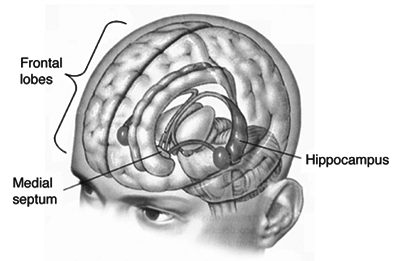
\includegraphics[width=0.5\textwidth]{img/brainareas.png}
    \caption{The brain areas mainly involved in storing and retrieving declarative knowledge \protect\cite{amnesia}}
    \label{fig:brainareas}
\end{figure}

Although the whole brain is involved in storing memories, the most prominent areas facilitating the process of memorising are the frontal lobes, medial septum and the hippocampus \cite{cognitivepsychology} (see figure~\ref{fig:brainareas}). The prefrontal regions are responsible for the creation and retrieval of memories, whereas the hippocampal and surrounding areas allow permanent storage of these memories. Because of this dynamic, \citeA{modalmemory} conceived a modal theory of memory, displayed in figure~\ref{fig:modalmemory}. In this model, information is perceived as sensory input, and is then shortly stored in the sensory memory. If the perceiver has paid enough attention to the input, it is then transfered (or encoded) into short-term memory. When the input is strong enough, that is, rehearsed often enough within short term memory, it can be more permanently stored in long-term memory. If not, the input fades away from memory and is forgotten. When a memory exists in long-term memory, it has to be retrieved into short-term memory in order to be remembered and used.

This model was heavily influenced by developments in electrical engineering and computer sciences, and can be thought of as functioning like a complex computer, where data is written on a hard drive (the long-term memory), and can be used by first retrieving it into working memory (or short-term memory) and later be transferred to the hard drive again (although within a computer the separation is much more clear, whereas short- and long-term memory might overlap more). However, the way the brain works is different from a computer in the sense that a brain has to put effort into memorising data, and that a brain forgets data over time. Therefore, instead of merely inputting the data, learning requires a more rigid approach.

\begin{figure}
    \centering
    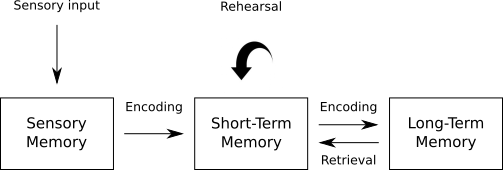
\includegraphics[width=0.5\textwidth]{img/modalmemory.png}
    \caption{The modal model of memory proposed by \protect\citeA{modalmemory}}
    \label{fig:modalmemory}
\end{figure}

\citeA{karpicke4} describes two seperate learning practices based on the modal model of memory, namely encoding and retrieval practices, where encoding practices are focused on meaningful encoding or construction of knowledge, and retrieval practiced are more focused on the reconstruction and rehearsal of knowledge. He states that both practices are essential to enhancing learning. Flashcards are a famous retrieval practice, which emphasise drilling the same pairs by association over and over again, whereas concept maps are known to be an encoding practice where the student has to connect diverse concepts within one topic by meaningful relations.

The following sections will elaborate on cognitive effects with regard to both encoding and retrieval practices, and relating them with their relevance to the effectiveness of concept mapping and flashcard systems respectively.

\section{Cognitive effects with regard to encoding practices}

The first step of memorisation is always encoding, because (logically speaking) a stimulus first has to be processed and encoded in either short-term or long-term memory in order to be retrieved or used later on. After all, one cannot retrieve a memory which is not already there. It therefore is important to first acknowledge by which means knowledge is encoded, and in what kind of structure it is then stored.

\subsection{Early metaphors for the brain}

For centuries, a lot of metaphors describing memory depicted the brain as a room in which a person could store physical things, for example as a library filled with books or a storehouse with items \cite{roediger}. This metaphor seems intuitive and is easy to understand, hence it is still prevalent today. There even exists a widely-used memorisation technique called the \emph{loci method}, which lets students are asked to imagine a house where they have to store memories as physical objects in the room. They can then later retrieve the memories by walking through the house along the objects they have stored the memories in \cite{cognitivepsychology}.


Yet, this model still has certain flaws. Firstly, with regards to retrieval practices, it depicts memories as static objects which only have to be stored to be remembered forever, misleading students, teachers and scientists into focusing more on encoding practices than on retrieval practices \cite{karpicke4}. Furthermore, memories are imagined as separate objects, which does not correspond with how memories are encoded in the brain. As a matter of fact, already in the 19th century, Cajal discovered that memories were patterns of electrical neural activity leading to synaptic changes \cite{longtermpotentiation}. This enabled another spatial metaphor, namely that of a switchboard, where the synapses were represented by electrical wires \cite{roediger}. Later on, when the field of computer science begun to emerge, this metaphor transformed to that of a computer, enabling the conception of the modal model of memory. This is already a more useful metaphor than the physical space metaphor, since it is more biologically accurate, and it emphasises the need of communication between certain nodes (encoding and retrieval between the different memory systems).

However, the metaphor of a computer still has its flaws. A computer stores information on certain independent addresses in the form of binary data, and thereby implies that one can store data for later use without any need for comprehension of the data, and that the data can be formatted in any way the user would like to. Yet, the brain is differently structured, which has consequences for succesfull encoding.

\subsection{The brain as an associative network}

Unlike a computer, the brain is not organised into bits with physical addresses, but rather structured as an associative network. This entails the data being stored and retrieved by means of associated peers. In the brain, the neurons function as the nodes, and the synapses function as the edges. When information is encoded, new neurons are marked, and these are connected to other relevant, already marked neurons in the network. When something then has to be retrieved from memory, neurons signal relevant neighbouring neurons in order to activate the relevant parts of the brain. More generally speaking, when stimulated with a retrieval cue, the brain can then use neural pathways to find a corresponding item in the brain. These networks are sometimes referred to as \emph{semantic networks}, and the implication for retrieval as \emph{spreading activation} \cite{cognitivepsychology}. This effect has also been found on a cognitive level, for example \citeA{kintsch} has found that material is often not literally encoded, but rather as a set of abstract meaning units representing certain associations between concepts.

\subsection{Elaborative processing}

Because information is retrieved in the brain via related nodes and edges in the semantic network, strong neural pathways facilitate the retrieval process. One way of creating these pathways is elaborative processing \cite{karpicke4, cognitivepsychology}, which focuses on meaningful processing of the content. \citeA{craik} conducted an experiment where students were to freely recall from a list of words after the students had to train the words by one of the following techniques: answering questions about structural details (e.g. is it in capital letters); about phonemical details (e.g. the word rhyming on another word); whether the word fits into a certain category; and whether the word fits in a certain sentence. They found that the more meaningful the task was, the higher the retrieval rate was (so the latter techniques were more effective). The same result was found by \citeA{barclay}. Furthermore, research conducted by \citeA{nelson} presented students with paired associates that where either semantic or phonetic (in this case rhymes), and students showed a significantly higher recall of semantic associates. These studies demonstrate the importance of meaningful processing for retention.

\subsection{Implications for concept mapping}

Reflecting on the previously described theory of associated networks, it appears that a semantic network is very similar in structure to concept maps, and thereby the maps provide an accurate representation of the way information is retrieved from the brain. For example, \citeA{canas} states that "the widespread use of concept maps is based on the notion that a concept map is a reflection of the builder's cognitive structure and thus portrays his or her understanding of the domain depicted in the map" (p. 1). \citeA{nesbit} speculate that because of this, more and better retrieval cues are created when learning from or generating a concept map. Furthermore, a concept map displays the relations between certain concepts, and thereby focuses more on the meaning behind the content, rather than just the content itself.

\section{Cognitive effects with regard to retrieval practices}

According to \citeA{karpicke4}, a lot of educational practices have placed an emphasis on finding optimal ways to encode knowledge and experiences, but that retrieval practices have received less attention. Nevertheless, basic research has indicated that retrieval is still important to consider in any analysis of learning. This is mainly due to the fact that information is not stored exactly and indefinitely, but rather that memories are forgotten over time. Two theories have been proposed and debated over explaining why forgetting occurs, namely by interference of other redundant memories and by decay of existing memories.

\subsection{Interference and Decay}

\label{subsec:interferencedecay}

The theory of interference being responsible for forgetting has been demonstrated in an experiment by \citeA{interference}. The participants were asked to memorise sentences in the form \emph{A \textless person\textgreater{} is in the \textless location\textgreater}, where sometimes multiple persons where associated with only one location, and some locations with only one person. They found that if a sentence contained locations or persons with multiple associations this had an impact on the recognition time for that sentence, and even more so if both the location and the person had multiple associations. The explanation for this phenomenon is that since memories are retrieved by means of spreading activation and only limited activation can spread from one source \cite{cognitivepsychology}, the activity has to be divided over different branches in the semantic network, increasing the retrieval difficulty of the correct node. The increase in difficulty is also related to as the \emph{fan effect}.

The effect of decaying memories takes place in the connections between neurons, and therefore it is important to first examine how neurons communicate signals. Figure~\ref{fig:neuron} displays a schematic representation of a neuron in which it can be seen how the soma (cell body) is connected via an axon to the dendritic tree of other cells. The neuron can transmit stimuli by creating an action potential in the nucleus, transmitting this signal through the axon to the terminal button in the connected telodendrion (in the image refered to as the terminal aborization). There, neurotransmitters are released from vesicles, and after they have crossed the synaptic cleft there is a certain chance of being received by postsynaptic receptors. When this is the case, the nucleus of the receiving cell is triggered via the connected dendrite to also create an action potential, and the whole process is repeated \cite{longtermpotentiation}. The strength of a certain connection between neurons is therefore dependent on the action potential generated by a nucleus, the amount of telodendria over which the action potential has to be distributed (hence the aforementioned fan effect), the amount of neurotransmitters in the terminal button, and the amount of postsynaptic receptors in the dendrite of the next neuron.

\begin{figure}
    \centering
    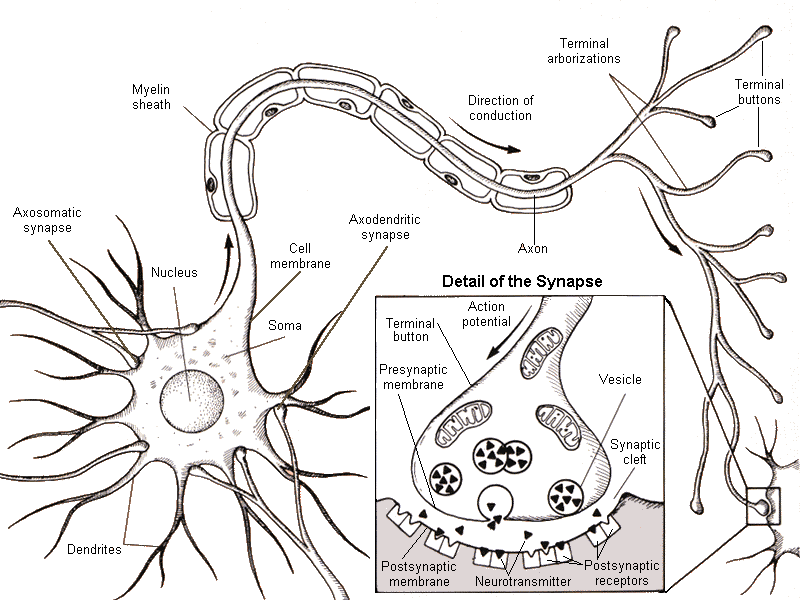
\includegraphics[width=0.8\textwidth]{img/neuron.png}
    \caption{A schematic image of a neuron with a closeup of a synapse \protect\cite{website:neuron}}
    \label{fig:neuron}
\end{figure}

One widely studied effect with regard to the increase and decrease of action potential and strength of memory traces is called long-term potentiation (LTP) \cite{cognitivepsychology, longtermpotentiation, activationbasedmodel, amnesia}. Whenever a neurotransmitter is received by by a receptor, not only is the next nucleus activated to release its action potential, but also more receptors are activated, so that the postsynaptic membrane is able to receive more neurotransmitters at the next activation. Furthermore, another process is activated altering the metabolical profile of the neuron, causing it to create proteins for more stable increased sensitivity towards stimuli. It is also speculated that there might be a retrograde effect, causing presynaptic modifications such as the creation of more neurotransmitters in the presynaptic vessicles \cite{longtermpotentiation}. This all results in an increased sensitivity in the postsynaptic neuron towards action potential in the presynaptic neuron, which then again increases the strength of this particular memory trace. Over time, if a specific neural pathway is not used, the effects of LTP decrease again, causing its strength to decrease and thereby causing decay. This also is a predictor for the \emph{testing effect}, the effect of retrieval strengthening memory more than extra opportunities for further encoding, even when the retrieval is only carried out internally without any outward response \cite{microlearning}.

Although both the effect of interference and decay have been proposed as separate theories and have been debated, they are still mutually inclusive, and \citeA{cognitivepsychology} therefore conludes that forgetting results both from decay and from interference.

\subsection{Power laws of forgetting and learning}

Now that the relevant theories for learning and forgetting have been discussed, it is important to investigate with which rate people learn and forget. Already in 1885, Ebbinghaus discovered the power law of learning, referred to as the inversal exponential nature of forgetting \cite{microlearning, activationbasedmodel}. The implication of this model is that memory not only systematically deteriorates with delay, but also that this loss is negatively accelerated, meaning that the rate of change gets smaller with increasing delay \cite{cognitivepsychology}. \citeA{wickelgren} already proposed the formula $m = \lambda (1 + \beta t)^{-\psi}$, where $m$ is memory strength (the probability of recognition), $t$ is time, $\lambda$ is the state of long-term memory at $t = 0$, $\psi$ is the rate of forgetting, and $\beta$ is the scaling parameter (see figure~\ref{fig:powerlawforgetting}). This formula has also found to be accurate by \citeA{wixted}. Finally, the effect has been directly related to LTP in the rat hippocampus by stimulating neural pathways directly with electrical signals \cite{raymond}.

\begin{figure}
    \centering
    \begin{subfigure}{0.7\textwidth}
        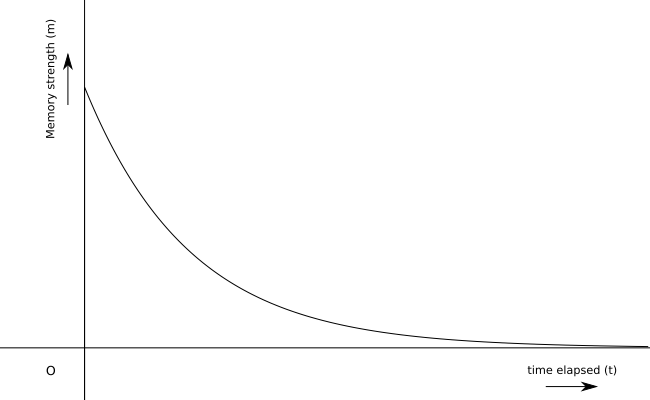
\includegraphics[width=\textwidth]{img/powerlawforgetting}
        \caption{The power law of forgetting, with m as the probability of recognition and t as the time passed since learning}
        \label{fig:powerlawforgetting}
    \end{subfigure}
    \par\bigskip
    \begin{subfigure}{0.7\textwidth}
        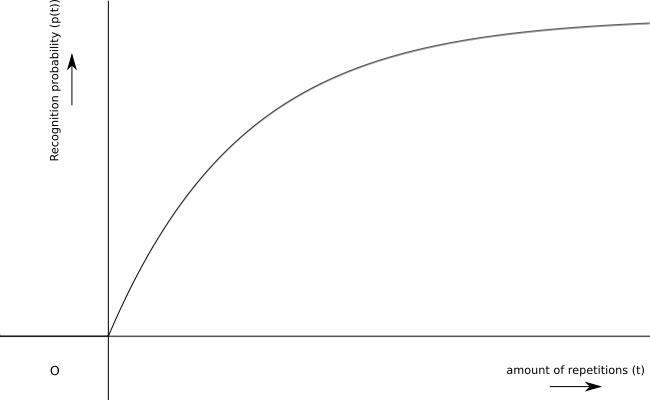
\includegraphics[width=\textwidth]{img/powerlawlearning}
        \caption{The power law of forgetting, with p(t) as the probability of recognition and t as the iterations of learning}
        \label{fig:powerlawlearning}
    \end{subfigure}
    \caption{The power laws of learning and forgetting}
\end{figure}

A similar effect has been found for the effectiveness of repetition: \citeA{powerlaw1} have proposed a power law of learning, stating that a learning curve is inversal exponential (see also \citeA{powerlaw2} and \citeA{powerlaw3}). \citeA{murre} propose $P = p(t) = 1-e^{-\mu_{i}t}$ as a function describing this power law, where $P$ or $p$ is the probability of recognition after $t$ iterations and $\mu$ is the learning rate of student $i$ (see figure~\ref{fig:powerlawlearning}). The power law states that repetition has a positive effect on retrieval probability. This effect however does not increase linearly but inverse exponentially, with an asymptote at a certain amount of repetition. Again, this effect has also been demonstrated in the context of LTP in rat hippocampi \cite{barnes}. The stronger memory trace from a higher repetition rate does not only result in a higher recall probability, but also in a more gradual retention curve, allowing memories to persist longer.

\subsection{Spacing effect}

\label{subsec:spacingeffect}

The spacing effect is a well known effect occuring within paired-associate learning, and demonstrates that repeated items are better remembered when both occurences are separated by other events or items than when they are presented in immediate succession \cite{verkoeijen, logan, siegel, xue, karpicke2}. This effect has been demonstrated with diverse populations \cite{verkoeijen, logan}, under various learning conditions \cite{verkoeijen, logan}, and in both explicit and implicit memory tasks \cite{verkoeijen}. Items in immediate succession are called massed items, and items in separated succession are called spaced items.

One can test the spacing effect either by using pure lists or mixed lists. When using pure lists, one compares the effect of learning a list containing only massed items with a list containing only spaced items, and using mixed lists one measures the effect of learning both massed items and spaced items in one list, comparing their individual retentions. \citeA{verkoeijen} state that the vast majority of studies are conducted using mixed lists and found that spaced items were consistently better recalled than massed items, yet studies using pure lists are relatively rare and have produced contradictory outcomes. They conducted a study providing participants first with an all-massed list, then letting them write down as many words as they could remember, and repeat an identical procedure for an all-spaced list with a 2 minute break inbetween. They conducted this experiment with short-lagged spaced items (with 1-4 items in between) and long-lagged spaced items (with 4-13), and found only a spacing effect in the latter experiment. However, \citeA{wahlheim} adds to this that repetition is only increases when a student detects the repetition of an item, and therefore the lag should not be too long.

Two theories have been presented explaining this phenomenon, namely the contextual variability theory and the study-phase retrieval theory \cite{siegel}. The first theory entails that because context is not static but continuous, and that therefore spaced items are studied in a greater variety of contexts and as such are easier to recall in yet other contexts than massed items due to the so-called encoding-specificity principle \cite{cognitivepsychology}. This principle entails that the probability of recalling an item depends on the similarity of the context during the encoding. The study-phase retrieval theory entails that additional retrieval cues for the repetition of an item are generated by earlier occurences and their associated contexts being associated with the repeated item. These theories are not mutually exclusive \cite{siegel}.

Inspired by the power laws of learning and forgetting, \citeA{karpicke} conducted an experiment to test the effect of constant or varying lags between items on learning. They tested this by conducting a similar experiment to \citeA{verkoeijen}, however in this experiment they only tested pure lists with three different lag intervals to test for an absolute spacing effect. For each lag interval category they tested for an expanding lag condition (where the lag would increase for the repetition of each next item), an equal lag condition (where the lag would remain constant) and a contracting lag condition (where the lag would decrease for the repetition of each next item) in order to test for a relative spacing effect. From their findings they confirmed the effect of absolute spacing, namely that longer gaps between items do have an effect on long-term retention, yet they did not find a relative spacing effect. However, this has not been tested for spacing with longer intervals, such as intervals spanning multiple days or weeks.

\subsection{Implications for the flashcard system}

\label{subsec:implicationsflashcards}

It can be concluded that the flashcard system derives its effects mainly from the testing effect by having students actively retrieve information instead of simply encoding it, and from the spacing effect by students going through the items interspersally instead of by immediate succession. The key question however is how often a single card has to be repeated. On the one hand, overlearning can occur, where the student repeats an item too often resulting in diminished learning effects because of the power law of learning, and also only on the short term \cite{rohrer}, which is inefficient. On the other hand, if the intervals are too long, students forget the items inbetween intervals, and then the spacing effect does not apply anymore. In order to solve this problem, most modern digital flashcard systems apply a system called \emph{adaptive spaced-repetition learning} (e.g. the Pimsleur system, the Leitner system, Supermemo, and Anki \cite{microlearning}). In this system, exponentially expanding intervals are used, not because of a relative spacing effect, but rather to increase the average (absolute) spacing with each new repetition. This creates a stronger memory trace every time, but also takes into account the further decreasing risk of forgetting because of the slower declining retention curve (see figure~\ref{fig:spacedrepetition}).

\begin{figure}
    \centering
    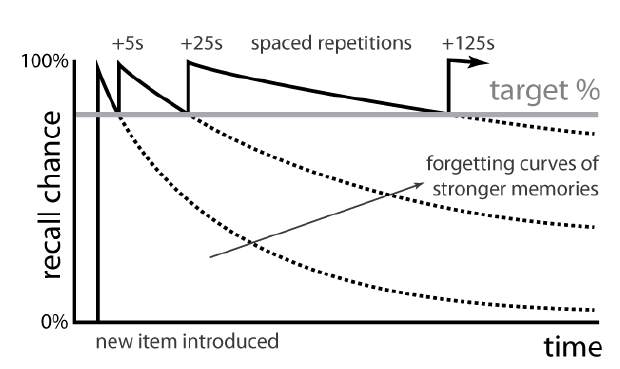
\includegraphics[width=0.5\textwidth]{img/spacedrepetition}
    \caption{Adaptive spaced-repetition learning (taken from \protect\citeA{microlearning})}
    \label{fig:spacedrepetition}
\end{figure}

\section{Conclusion}

Overall, this chapter has discussed several cognitive theories related to the storage and retrieval of explicit (or declarative) knowledge in and from the hippocampus. Related to encoding practices, it has now been established that the brain works as an associative or semantic network, and that meaningful or elaborative processing is important for the later retrieval of memories. This seems to fit with the structure and process of concept mapping, although more research is needed in this area. Furthermore, the theories of interference and decay have been discussed in order to explain forgetting of memories, together with Long-Term Potentiation and its effects on the rate of forgetting and learning. In addition, articles were discussed demonstrating that spaced rehearsal is more effective than massed rehearsal. This has finally led to the conclusion that adaptive spaced-repetition learning is an effective method to expand absolute spacing, which entails that items are repeated with exponentially increasing intervals.
 %Reviewed by Tobias, Paulina

\part{Design Report}
    The \nameref{ch:problem} mainly described the needs which the Flashmap System might be able to accomodate, and on page~\pageref{sec:intro_flashmap} generic features of such a system are described. Although the term Flashmap System is intended for describing any system including these features, when having to evaluate the idea one has to evaluate one or multiple specific implementations of that idea. Therefore, this part specifies the design features of the specific tool developed within this project, along with arguments in favour of and against these choices and their considerations, and the process with which they are incorporated within the tool itself. The design process is based on the Generic Model \cite{genericmodel}, which is displayed in figure~\ref{fig:genericmodel}.

\begin{figure}[h]
    \centering
    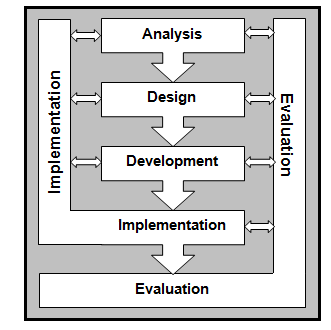
\includegraphics[width=0.5\textwidth]{img/genericmodel}
    \caption{The generic model by \protect\citeA{genericmodel}\label{fig:genericmodel}}
\end{figure}

The first chapter, \nameref{ch:analysis} on page~\pageref{ch:analysis}, describes the design implications stemming from the context, learner, and learning task of this project. The next chapter, \nameref{ch:frameworks} on page~\pageref{ch:frameworks}, describes implications from theoretical design frameworks relevant to the design of the flashcard and flashmap system. Finally, the \nameref{ch:software} chapter on page~\pageref{ch:software} describes the actual implementation of the software following from the design implications of the previous chapters.
 %Reviewed by Tobias TODO: Enlist separate aspects of the product
    \chapter{Analyses}

\label{ch:analysis}

Before designing an educational product, it is important that the designer first acquaints himself with the extrinsic factors important to this product. In order to discover the important characteristics of these factors, \citeA{instructionaldesign} enlist three types of analyses to be conducted, together with steps for conducting them. These are an analysis of the context, encompassing the needs of the users, and the environmental characteristics, an analysis of the learner, and an analysis of the learning task. Although these analyses are more targeted towards instructional design, and therefore more focused on a specific group being taught specific content, these analyses will still provide relevant information for the design choices and the evaluation. However, the steps will be adjusted and generalised or even omitted in order to fit the design of the more generic learning tool. The information gathered in order to conduct these analyses mainly stems from meetings with one of the teachers. This might not be the most reliable source of information because of the lack of triangulation, and should therefore not be taken as insight in the curriculum of Dutch Literature courses in secondary education, but rather as context information relevant to the design.

\section{Analysis of the learning context}

As already stated in the \nameref{sec:intro_evaluation} section on page~\pageref{sec:intro_evaluation}, the evaluation of the flashmap system will be evaluated within the Dutch secondary school Stedelijk Lyceum, with students having to learn about the Renaissance genres in Dutch Literature. This context will be further investigated within this section, starting with the Needs Assessment \cite{instructionaldesign}. Because although the general needs for a flashmap system are already described in the \nameref{ch:problem}, it is still important to investigate the specific needs of the context where the programm will be implemented.

\subsection{Needs assessment}

According to \citeA{instructionaldesign}, the first step in a needs assessment is to assess whether there is a problem, and what the nature is of the problem (see figure~\ref{fig:needsassessment}, mostly to identify the problem, but also in order to assess whether the innovation model or the discrepancy model applies for determining the needs. The first step is to assess whether there really is a problem in order to establish the general need. During the meetings, the teacher did confirm the need for better retention and comprehension of the content, and indicated that most of the time the students only learned the night before the exam in order to get a high (enough) grade and consequently forget everything again. This is not only wasteful of the effort of learning, but also causes problems when the knowledge becomes relevant again in the next chapter. The cause of this problem therefore definitely lies within the learning process, and could possibly be improved by the use of a flashcard or flashmap system, so it can be concluded that there is indeed a problem caused by learning, and it is thereby useful to proceed with the next phase of the assessment. Finally, \citeA{instructionaldesign} finally state that if there already exists instruction for the relevant learning goals, since if so than one has to proceed by using the discrepancy model, and otherwise by using the innovation model. The new tool is only there to enhance the current learning process by adding an additional activity, rather than adding new learning goals to an empty space in the curriculum. Thereby, from an instructional perspecticve, the flashcard or flashmap system is only an improvement of the currently existing instructional activities rather than a new innovation, and therefore the discrepancy model will be used.

\begin{figure}
    \centering
    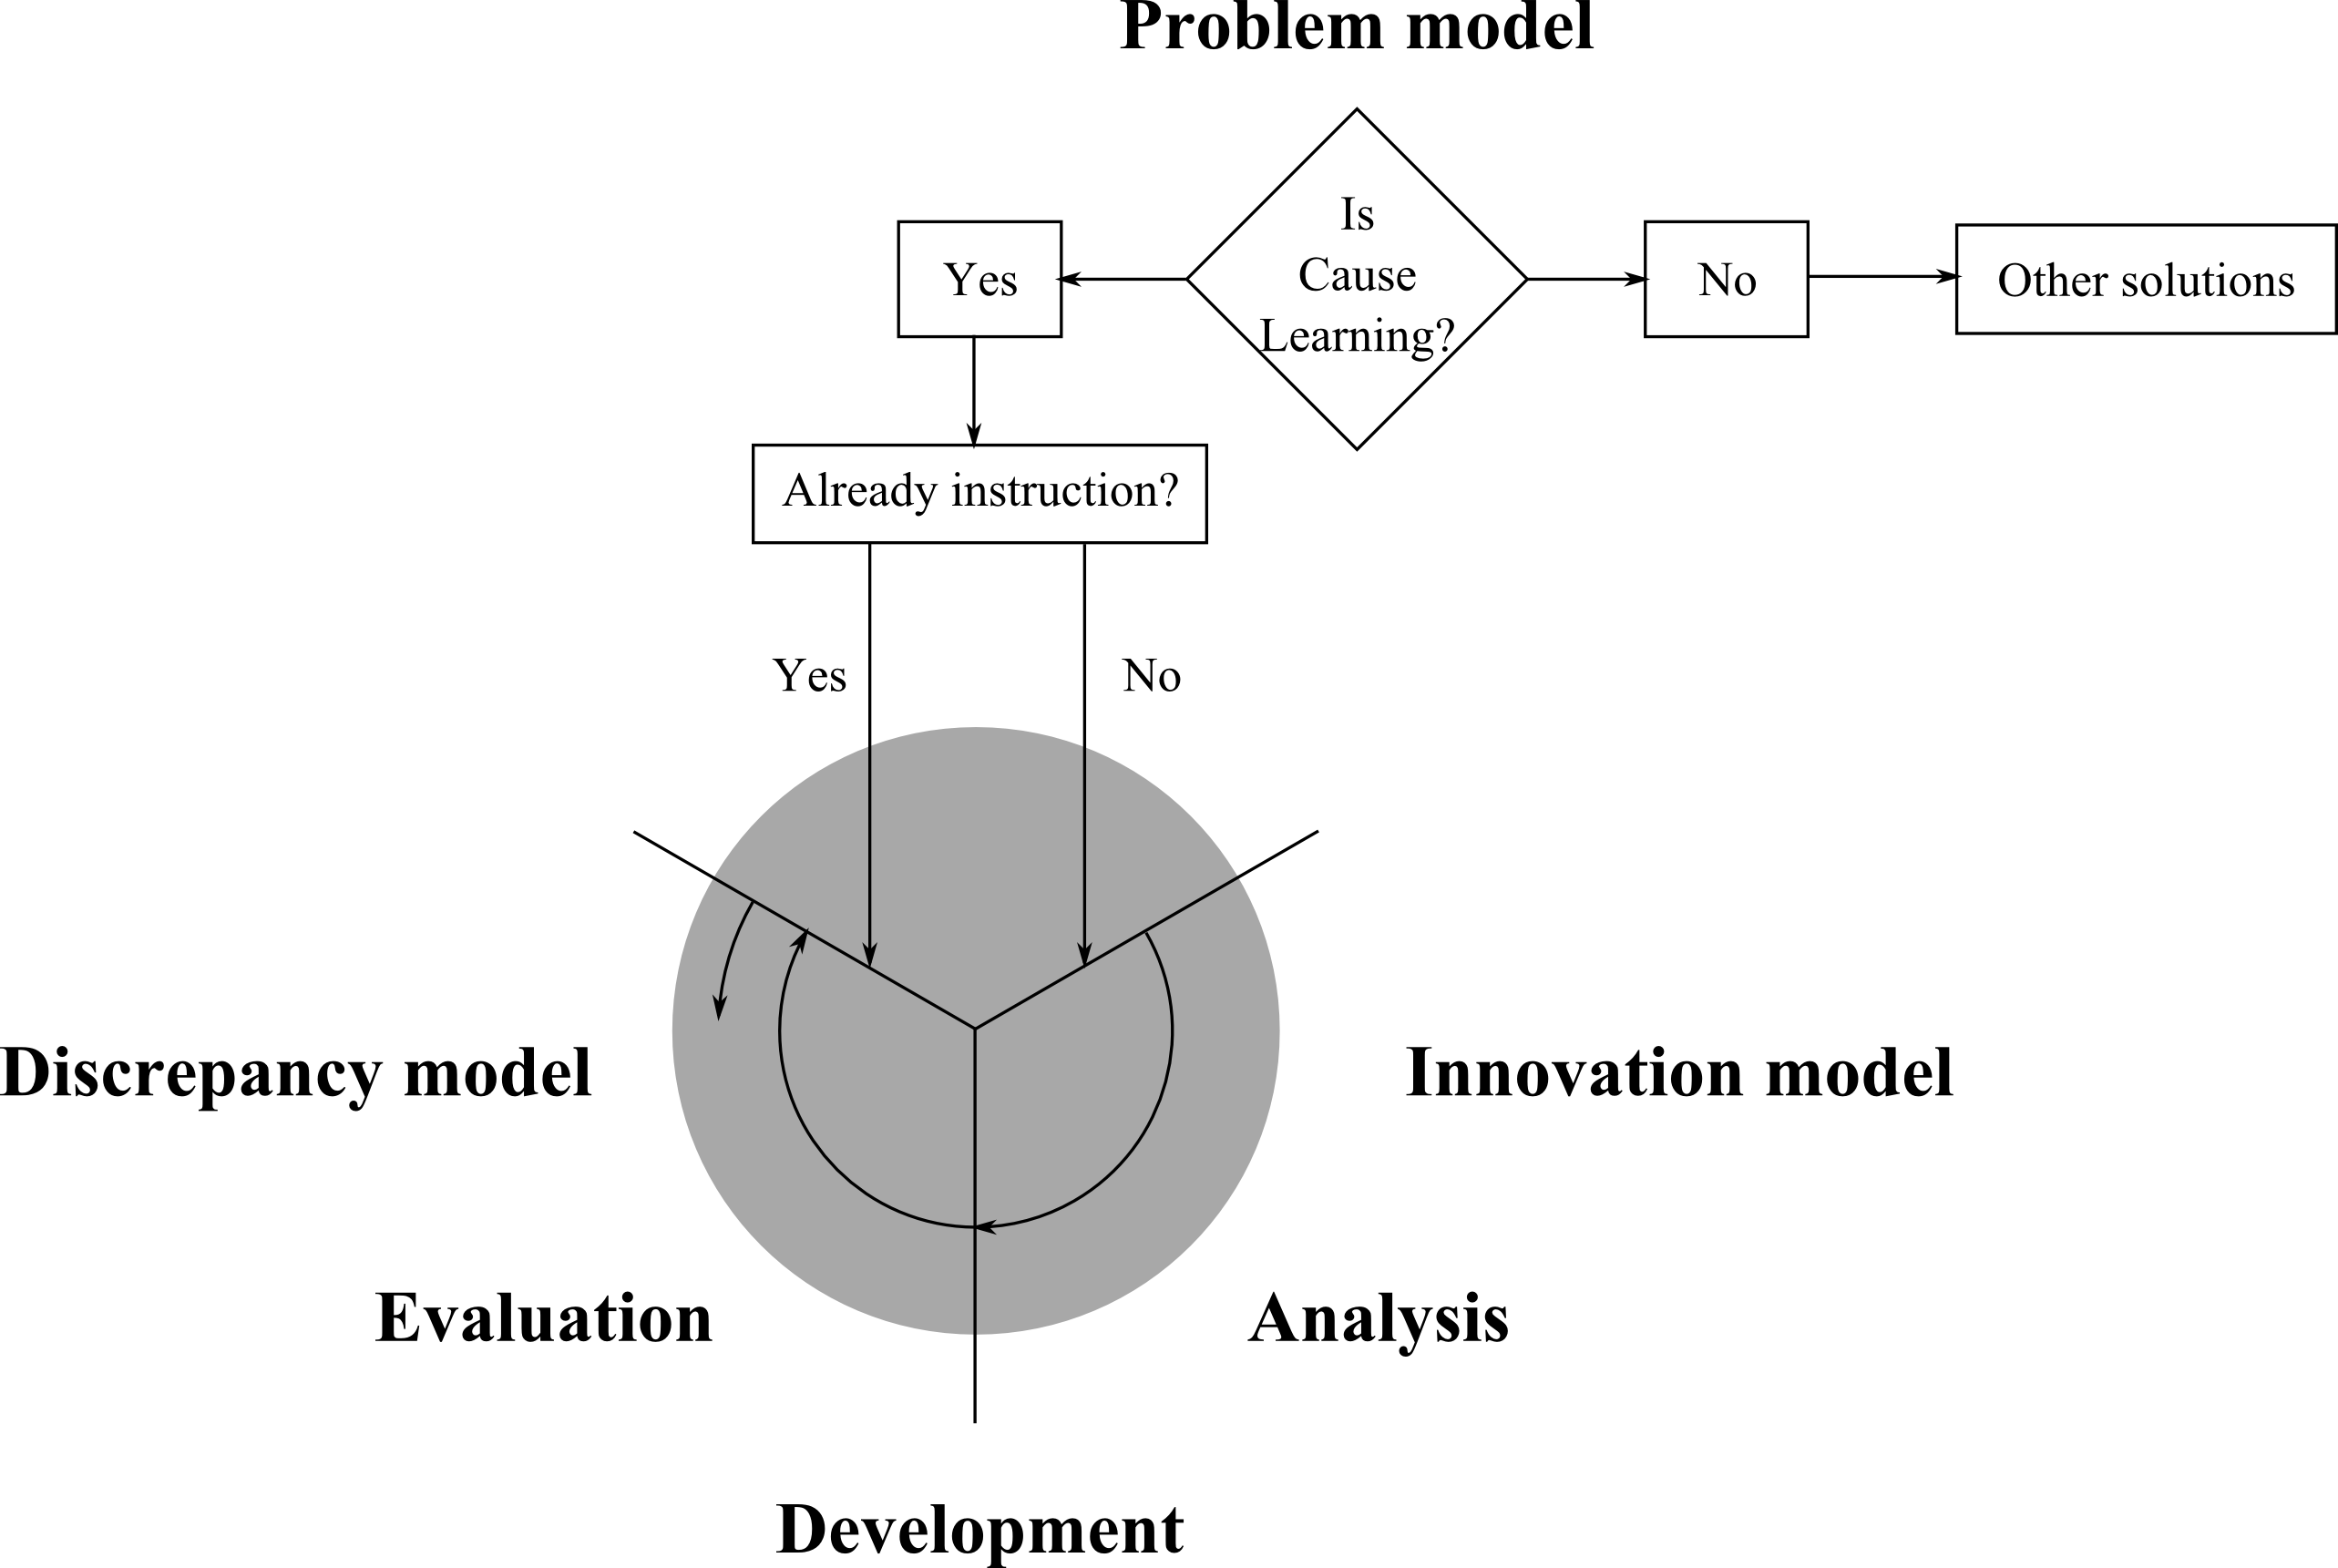
\includegraphics[width=\textwidth]{img/needsassessment.png}
    \caption{The three sides of needs assessment \protect\cite{instructionaldesign}}
    \label{fig:needsassessment}
\end{figure}

As can be seen in figure~\ref{fig:needsassessment}, the discrepancy model for needs assessment uses evaluative methods rather than analytical in order to establish the needs within the organisation. These methods include establishing the goals of the instructional system, determining how well these goals are currently being achieved, determining the gaps, prioritising the gaps, and determining which gaps are instructional needs (or in this case, educational needs). These remaining gaps can consecutively be used as a basis for determining the general use cases of the educational product. Normally an instructional designer tries to come into the organisation as a tabula rasa, without any preconceptions on what he would want to achieve and merely try to solve the real problem apparent in the organisation itself. However, because this design is theory driven rather than problem driven, it was merely checked with the teacher whether the problems stated in literature are also a problem here.

The first step was to confirm whether the goal stated by \citeA{glaserfield} of wanting students to memorise many facts in a meaningful way. Upon prompting the teacher what she deemed to be most important for her students to take away from her lessons was for them to become more familiar with the Dutch Renaissance writers or work. For example, she stated that she wanted the students to at least recognise important names when they saw a street name such as the "P.C. Hooftstraat" or the "Vondelpark". She also would like the students to be able to distinguish between different genres of literature, such as the \emph{sonnet} or \emph{emblematiek}. Based on these statements, the goals within the context are in line with students memorising and understanding all of the facts, without them being too ambitious. There are also differences between her and the other two teachers, they namely only offered the materials presented within the books, whereas she offered some additional content which the students also needed to master. However, she also stated that she would be responsible for the extra materials, and that the tool could be only to learn the textbook materials. Finally, she provided a test from the previous year to offer some more concrete examples of what she wanted the students to know, of which an English translation is included in the appendix on page~\pageref{ch:exampletest}. From this test, more goals can be extrapolated, such as students having to not only distinguish different genres, but also to define them or provide characteristics, and recognise the application of these features in both examples of the time periods as well as modern examples. Furthermore, they have to be able to relate the famous writers and writings to the genres.

According to the teacher, the students were mostly able to score points on the reproduction questions, such as having them to provide definitions or enlisting characteristics of genres. Thereby, most students were able to (barely) pass the test, which was already regarded as an important achievement, however minimal it might be. In this regard, the teachers already had scaled down their expectations of the students quite a bit to a realistic and feasible bar. The teacher also tried to make the material more appealing by focusing on examples, with succes.

However, as already indicated before, the main problem of students learning just before the exam and then forgetting about it remained an issue for the teacher, and more improvements could be made towards creating an understanding of the content by the students. Furthermore, although the examples make the content more appealing, according to the teacher students generally still did not experience the topic of Dutch renaissance literature as engaging or interesting (see also \citeNP{heemskerk}). Finally, most of the students would rapidly forget what they have learned after the exam, which the teacher did experience as wasteful. Therefore, the general categories of improvement can be enlisted as the students insufficiently understanding the content, not being immersed or engaged with the content (adequately), and retaining the acquired knowledge for a too short period of time.

Within the context of the Flashmap system, for now only the insufficient comprehension and retention of the content are prioritised, since there is no real evidence within the studied literature that the tool would also make content more immersive (although this could still be a side effect of the tool). These gaps are both instructional needs and are therefore appropriate gaps to tackle within the design.

\subsection{The learning environment}

\subsubsection{The school}

The Stedelijk Lyceum is one of the two major schools in Enschede (together with the Bonhoeffer College), which has an open denomination and provides education to 3339 students. It consists of 7 minor schools on different locations, of which the Kottenpark location is approached within this project. The location was approved by the Dutch Inspection of Education \cite{inspectierapport} based on analysing relevant documents, visiting the school and observing lessons, conduct interviews with relevant agents (such as teachers and students), and discussing the results with the director and administrator. They reported that the school climate is very positive and safe, and that the teachers have enough professional space to develop themselves. However, they also found that the exam results are some years around the national average, and some years below. The possible reasons they provided were that teachers usually focus on what students have to do instead of what they have to learn, and that they apply differentiation to a lesser extent. Yet, the school now makes use of student monitoring systems, so that they can better tackle problems like language deficiencies and the like.

\subsubsection{The curricular spiderweb}

Although \citeA{instructionaldesign} do enlist some of the steps necessary for describing the learning environment, \citeA{curricularspiderweb} provides a more widely used and thorough model, and therefore this will be used instead. This model is depicted in figure~\ref{fig:spiderweb}, and displays the relevant components which have to be taken into account for implementation of educational innovations. They are arranged as a spider's web, nog only illustrating their many inter-connections, but also underlining the vulnerability of the whole implementation. These aspects will be visited one by one from the perspective on the school, since the learner will be addressed separately in the next section.

\begin{figure}
    \centering
    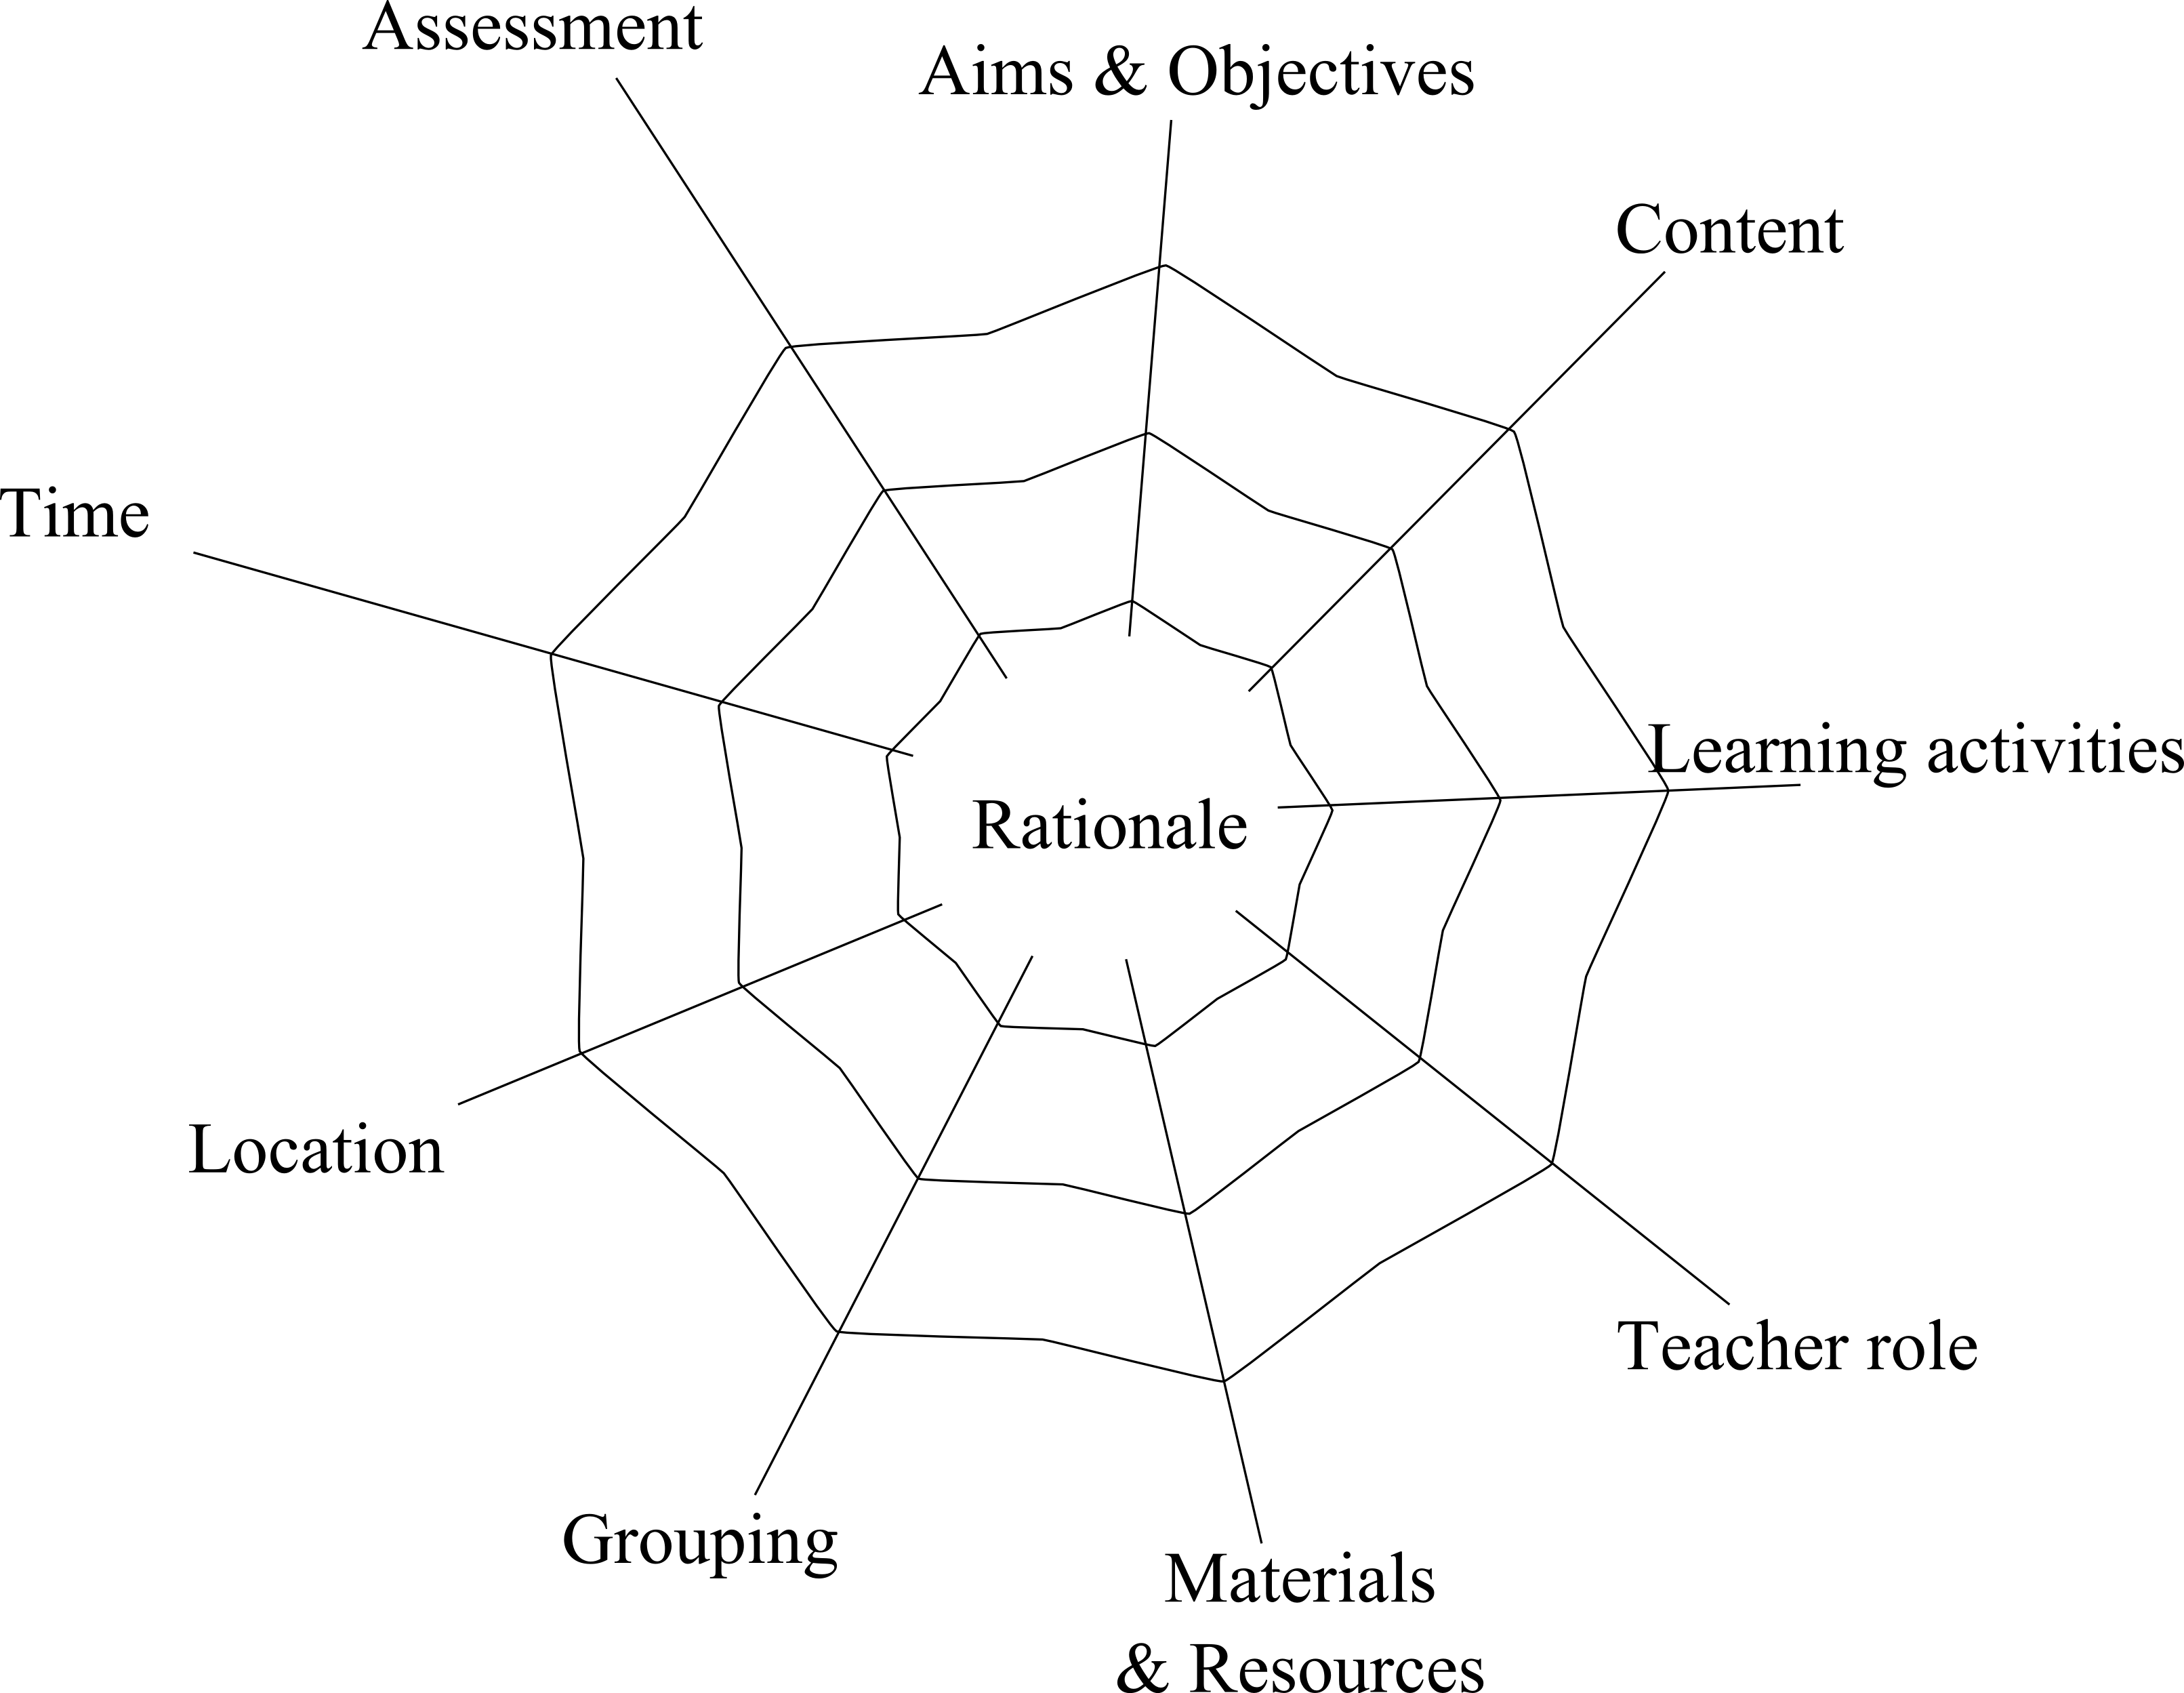
\includegraphics[width=0.7\textwidth]{img/curricular_spiderweb.png}
    \caption{The curricular spiderweb \protect\cite{curricularspiderweb}}
    \label{fig:spiderweb}
\end{figure}

The central aspect, \emph{rationale} (or vision), represents the question why students are learning the content in the first place. From the previously visited educational philosophies, one could make many arguments why students should familiarise themselves with Dutch renaissance literature: from a perennialistic or essentialistic perspective one could argue that it is the only way this knowledge can be transferred to the next generation and keeping it relevant; a progressivist could argue that one should first be familiar with older genres before one improve upon them or create new genres; reconstructivists might deem it important since it explains something about the national heritage, and thereby point out the flaws of the old ways; and finally an existentialist sees art in general as a meaningful way for self discovery. This intrinsic motivation is heavily dependent on the individual motivations and philosophy of the teacher. Most of these arguments are represented in diverse Dutch opinion pieces (e.g. \citeNP{opinion1, opinion2}). In the case of the consulted teacher, the arguments provided seemed to come mainly from the perennialistic and essentialistic perspective, namely that the content is part of our cultural identity and thereby important \emph{an sich}. However, she also indicated the existentialist self-discovery to be valuable. Furthermore, schools are extrinsically motivated to teach the material, since it has to demonstrate to society (mainly the exam committee) that their students have mastered this content. This is mainly related to subdomain E2 and E3 in the Dutch national exam programm, which states that a student can recognise and distinct between literary textgenres, and apply literary concepts in the interpretation of literary work; and that a student can provide the outlines of the (Dutch) literature history, and place literary works in this historical perspective.

Both the content and aims \& goals are already stated in the needs assessment, and can be summarised as: Students have to learn about prominent writers and genres within the context of Dutch renaissance literature; and have to be able to recognise important names and concepts, be able to define them or relate them to each other, and apply features of genres in examples of texts.

The course consists of two different types of learning activities, which are classroom instruction, and individual learning at home by the students. Their are two sessions of classroom instruction, both lasting 50 minutes, in which the 100 students are divided over the three teachers in static groups on separate locations. These lessons take place over the course of two weeks, with one lesson provided in one week. Within these lessons, the teachers transfer knowledge and provide excersises for the students. Outside of the lessons, the students still have to study the textbook Laagland individually \cite{laagland}, which contains all of the materials which will be prompted on a final written assessment. As already stated before, the teacher indicated this activity mostly to take place on the evening before the assessment, and only on a superficial level. Finally, this assessment takes place in the second week after the final instruction, and will be similar to the example test included in the appendix on page~\ref{ch:exampletest}.

The teacher stated that the course mainly consisted of the rote memorisation of facts, and that she was still doubtful whether the students would actually be willing to participate in the evaluation of the Flashmap system. Yet, she did see the general use of the tool for achieving the learning goals, and therefore still seemed to be enthusiastic in cooperation and encouraging the students to participate. The only two technical problems are that there is not too much time for extra activities within the lesson plan and the teachers being quite busy themselves, and that the technological possibilities within the classroom are limited. Within the classroom, only a couple of computers are available for use, and still run relatively old software. Therefore, the activities envolved in using the flashmap have to target the individual learning of students, since they have more time outside of the lesson plan, and mostly do possess the hardware and software necessary to run the software.

\section{Analysis of the learner}

In order to tailor to the specific needs and interest of the students themselves, it is important to also investigate the characteristics of the learner. \citeA{instructionaldesign} propose a methodology for assessing a learner which focuses on two axes: Stable and Changing, and Similarities and Differences, creating 4 categories. Within these categories, different types of learner characteristics, which are enlisted in table~\ref{tab:catslearner}. Stable similarities involve characteristics which are similar among people and do not change over time, such as sensory capabilities and their corresponding perceptual responses, the way people process information, and finally the ways and conditions in which people learn. Stable differences relate to characteristics different among people but stable over time, such as certain aptitudes, cognitive styles, psychosocial traits, or inheritary traits such as gender, ethnicity \& racial group. Changing similarities are similarities that do change over time, these characteristics are mainly attributed towards development processes. Finally, changing differences are differences in development accross people, which can mainly be attributed towards different upbringings or interests. Instead of visiting the learner characteristic according to each above mentioned category, \citeA{instructionaldesign} propose an more conveniently arranged outline which will be used in the next sections, albeit slightly altered in order to fit the current project.

\begin{table}[ht]
\centering
\begin{tabular}{l|l|l|}
         & Similarities                                                                                                                      & Differences                                                                                                                        \\ \hline
Stable   & \begin{tabular}[c]{@{}l@{}}Sensory Capacities\\ Information processing\\ Types and conditions of learning\end{tabular}            & \begin{tabular}[c]{@{}l@{}}Aptitudes\\ Cognitive Styles\\ Psychosocial traits\\ Gender, Ethnicity, \& Racial Group\end{tabular}    \\ \hline
Changing & \begin{tabular}[c]{@{}l@{}}Development Processes:\\ - Intellectual\\ - Language\\ - Psychosocial\\ - Moral\\ - Other\end{tabular} & \begin{tabular}[c]{@{}l@{}}Developmental state:\\ - Intellectual\\ - Other\\ Prior learning:\\ - General\\ - Specific\end{tabular} \\ \hline
\end{tabular}
\caption{The four categories of learner characteristics \protect\cite{instructionaldesign}}
\label{tab:catslearner}
\end{table}

\subsection{Physiological characteristics}

\label{subsec:physiologicalchar}

The students who will participate in the research are enrolled in grade 4 of Dutch secondary education, and therefore should be around the age of 16-17, with some deviations due to students either having skipped or repeated a grade. Therefore, the students are generally considered to be either at the end of puberty, or the beginning of young adolescence. Chapter \refname{ch:theory} on page~\pageref{ch:theory} already provides general theories about the learning process within the brain. However, during late puberty and early adolesence, the brain is still heavily in development, especially the prefrontal cortex. \cite{blakemore}. These changes might be even more relevant than the pure chronological age, and therefore they will have to be elaborated on further before delving into the cognitive characteristics.

\begin{figure}
    \centering
    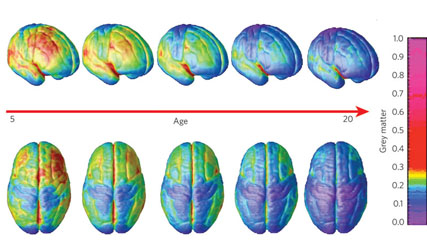
\includegraphics[width=.7\textwidth]{img/braindevelopment.png}
    \caption{The MRI scans from the longitudinal study conducted by \protect\citeA{giedd}, showing the maturation of the brain during childhood and adolescence}
    \label{fig:braindevelopment}
\end{figure}

In order to map out the changes in the adolescent brain, \citeA{giedd} performed a longitudinal MRI study of the brain development during this period, of which the results are displayed in figure~\ref{fig:braindevelopment}. Within this study, three themes emerged within the adolescent development of the brain:

\begin{enumerate}
    \item After a peak in growth of both braincells, connections and neurotransmitters during childhood, one can see a decline in adolescence;
    \item The connectivity between different regions of the brain increases;
    \item A new balance is formed among frontal and limbic lobes.
\end{enumerate}

The first theme is a result for the brain becoming more streamlined after having collected a lot of information during late childhood, making it more efficient (see also page~\pageref{subsec:interferencedecay} on \nameref{subsec:interferencedecay}). This is also known as peak plasticity, which after that again decreases over time. \citeA{powell} describes this phenomenon as \emph{Use it or lose it}, since the brain rigorously selects the specific memories which are activated during this time. The second theme refers to the strengthening of specific memories, which are enhanced during that period. Finally, during adolescence a shift is made from "cold" to "hot" cognition, where the former relates to hypothetical, low-emotion reactions, and the latter to high arousal decision making, strongly influenced by peer pressure and real, direct consequences. This is strongly related to the prefrontal cortex being strongly developed, resulting in the teenage brain to rely stronger on the amygdala: the more emotional, impulsive area of the brain.

The developmental level of the prefrontal cortex has also been found to positively correlate with the IQ of students, more so than other regions of the brain, which is an indication of this development to be the most influential for the cognitive development within adolescents.

The development of the prefrontal cortex has important consequences for the cognitive development of adolescents. They become more capable of abstract, multidimensional, planned and hypothetical thinking in comparison to children \cite{steinberg}. Adolescents also tend to use their hippocampus more often during executing certain tasks \cite{finn}, possibly due to the highly increased plasticity of the brain.

\subsection{Cognitive characteristics}

The Dutch highschool is subdivided into three main categories, which are VMBO, HAVO and VWO, ranking from lower to higher rates of academic achievement and expectations. The students targeted within this projects are VWO-students, which means that they are most likely to have a relatively high IQ, and are quite apt of learning and passing for written tests. Furthermore, at the beginning of grade 4 of VWO, students are allowed to choose between a nature profile or a society profile, determining whether they have respectively have more STEM subjects (such as math or biology), or more subjects related to language, humanities or economy. Therefore, where students who chose the nature profile are generally more apt to apply logic to technical problems, those who chose the society profile are generally more apt and used to learning information by reading texts. This makes up for different specific aptitudes within this specific Dutch literature course, where reading skills are more relevant. VWO-students are also subdivided into Gymnasium and Atheneum students, where the former group outside of the regular curriculum also has to learn classical languages (Latin and Ancient Greek) and culture. Because the Dutch renaissance literature has a lot of connections with classical genres, Gymnasium students might have an advantage in prior knowledge. Furthermore, all students should have learned about the relevant time period in their history classes prior to this course (e.g. the Spanish War, the Lutheran reformation etc.), providing with the relevant knowledge to understand the context of Dutch renaissance literature. Finally, the students have received a similar instruction on Dutch medieval literature, which is also relvant for concepts in the renaissance literature, such as the \emph{Mecenas}, the \emph{Lyriek} and \emph{Rederijkers}.

\subsection{Social characteristics}

This section covers the stage of moral development, the socioeconomic status, the racial or ethnic background, and the religious denominations of the students. The stage of moral development is relevant since it influences the individual decisions the students are likely to make. The socioeconomic status (SES) is found to influence the academic achievement of students, since they are predictors of both the safety of the home situation and the support from the parents. Furthermore, racial and ethnic backgrounds might influence the attitudes that students have towards certain topics. Finally, since the subject of Dutch renaissance literature is heavily influenced by religion, especially the reformed church, the denomination influences the perspective of the student towards the subject, and determines a certain amount of prior knowledge. The SES, the racial or ethnic background, and the religion have not been investigated within the target group, so instead public available statistics from the Dutch social and cultural plan agency (\emph{Sociaal en Cultureel Planbureau}, SCP), the Ministry of the Interior and Kingdom Relations (\emph{Ministerie van Binnenlandse Zaken en Koninkrijksrelaties}, BZK),  and Statistics Netherlands (\emph{Centraal bureau voor de Statistiek}, CBS) were used.

%The region around Enschede has a lesser income in comparison to the national income: where the national average lies around 33.2 thousand euros, the average income in Enschede is 27.1 thousand euros per household. This is also true when looking at the median (28 vs 23.1 thousand) and for the average and median standardised incomes (23.5 vs 19.7 and 20.9 vs 17.9 thousand euros), where the latter are corrected for differences in size and composition of a household (see also table~\ref{tab:income}). 

Every four years the SCP publishes data reporting the socioeconomic status (SES) of postal areas in the Netherlands \cite{scp}. The SES is based on three variables of the people living their, namely their education, their spendable income, and their position on the labour market. The data about the postal area of the school is displayed in table~\ref{tab:scpses}, together with the data of its two major neighbouring postal areas. As one can see, all of the values are below the national average SES, and that the surrounding postal areas have a lower SES than the school's postal area. However, academic achievement and socioeconomic status are highly correlated \cite{academicsocioeconomic}, and given that the approached students are enrolled on the VWO level one might expect them to come from households with higher incomes. Furthermore, the BZK frequently publishes indications of living circumstances \cite{bzk}, which is specified with smaller areas and is found to correlate with the SES \cite{knol}. On this map, the area Bolhaar scores a 0.3 in comparison to the national average. It could therefore be that the actual SES of the students of the school is somewhat higher than indicated within the table, especially since there is also a university campus within the same postal area, where low income university students live.

\begin{table}[]
    \centering
    \begin{tabular}{|p{2cm}|p{2cm}|p{2cm}|p{2cm}|p{2cm}|}
        \hline
        Postal code & Number of residents & Number of households & SES score & SES rank \\ \hline
        National &  &  & 0.28 &  \\ \hline
        7521 & 9555 & 4624 & -1.28 & 3254 \\ \hline
        \textbf{7522} & \textbf{7100} & \textbf{4551} & \textbf{-0.37} & \textbf{2792} \\ \hline
        7523 & 12180 & 6060 & -1.62 & 3333 \\ \hline
    \end{tabular}
    \caption{Indicators of socioeconomic status on both national and postal code levels \protect\cite{scp}}
\label{tab:scpses}
\end{table}

%Racial/ethnic background, affiliations

Among other data, the CBS offers descriptives of students, categorised per national district. This descriptive data entails information about the age, sex, type of education, and ethnicity of students, and the interactions among these variables \cite{cbsethn}. From this data, descriptives about 16-17 year old students from Enschede enrolled in vwo grade 3-6 was extracted, displaying their age and ethnicities. 23.06\% of the 16-17 year old students are enrolled in VWO, where 43.97\% is male and 56.03\% is female. The distribution of ethnicity is visualised in figure~\ref{fig:ethnicitychart}. 76.56\% of the students are native and 31.09\% are non-native. 9.16\% of the students is western non-native, and 21.92\% is non-western non-native. The CBS defines a non-western non-native as an non-native originating from Afrika, Latin-Amerika and Asia (except for Indonesia and Japan) or Turkey. The most prevalent non-western ethnicity is Turkish, with 8.08\%.

\begin{figure}
    \centering
    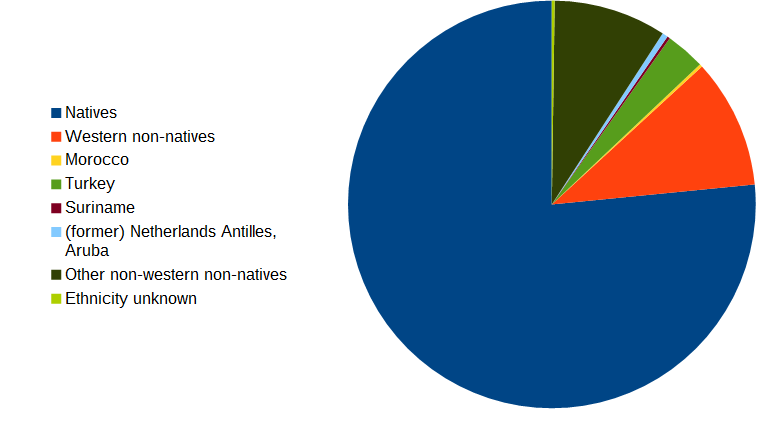
\includegraphics[width=0.7\textwidth]{img/ethnicitychart.png}
    \caption{The distribution of ethnicities among 16-17 year old vwo students of education type vwo3-6 \protect\cite{cbsethn}}
    \label{fig:ethnicitychart}
\end{figure}

Finally, the CBS also offers statistics about religious denominations \cite{cbsdenom}, which state that 57\% of the people in the province of Overijssel is affiliated to a church. These affiliations are split up in different religions: 22\% Roman-Catholic, 8\% Protestant, 12\% Dutch Reformed, 7\% Continental Reformed, 4\% Islam, and 5\% miscellaneous (see figure~\ref{fig:denominations}. 43\% is not affiliated to any church, however this does not necessarily entail that they do not have a religious worldview. Data is also offered on how frequent people visit the church: 14\% visits every week or more often, 4\% two or three times a month, 4\% once a month, 8\% less than once a month, and finally 70\% (almost) never (see figure~\ref{fig:churchvisits}. This would indicate that although there is a majority affiliated with a certain church, most of the people do not actively take part in their respective community. There are also more specific statistics available about the region of Twente only \cite{cbsdenomold}, however these are older and might already have changed significantly over the last 13 years. Yet, they state that Twente is more religious than the overal province of Overijssel. Unfortunately, there are no statistics available about Enschede only. Finally, the school of the target group has an open (i.e. non-religious) denomination, whereas the other large school in Enschede has a christian denomination, so one might expect mainly the students without any strong religious views to choose for this school.

\begin{figure}
    \centering
    \begin{subfigure}[b]{0.7\textwidth}
        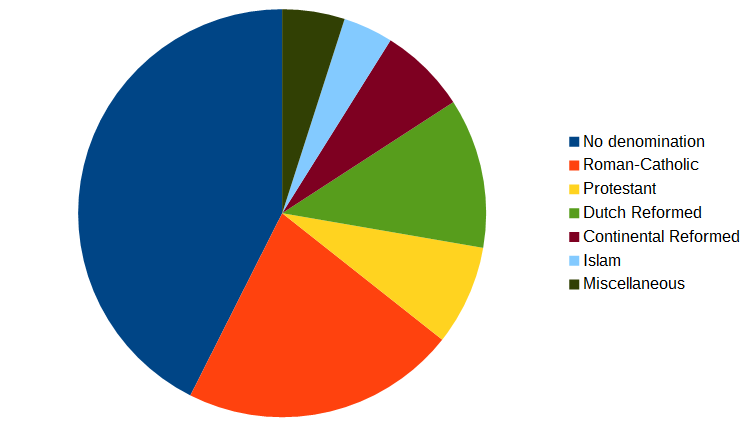
\includegraphics[width=\textwidth]{img/denominations.png}
        \begin{center}
            \caption{A distribution of church affiliations}
            \label{fig:denominations}
        \end{center}
    \end{subfigure}
    \begin{subfigure}[b]{0.7\textwidth}
        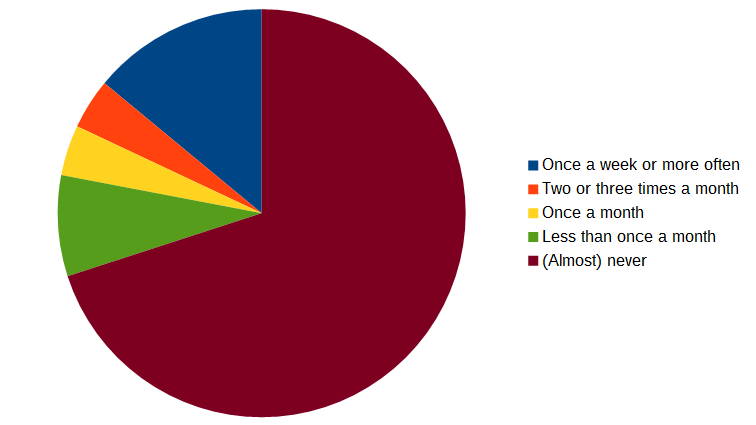
\includegraphics[width=\textwidth]{img/churchvisits.png}
        \begin{center}
            \caption{The distribution of frequencies of church visits within the group of people affiliated to a church}
            \label{fig:churchvisits}
        \end{center}
    \end{subfigure}
    \caption{Denominations within the region of Twente \protect\cite{cbsdenom}}
    \label{fig:religion}
\end{figure}

\subsection{Affective characteristics}

The influences on the students attitudes can be mainly categorised into two factors: the natural factors and the nurtural factors, which will be described in seperate paragraphs below.

Within the section \nameref{subsec:physiologicalchar} on page~\pageref{subsec:physiologicalchar} it was already described that students rely mainly on their amygdalic systems instead of their prefrontal cortex during young adolescence. According to \citeA{steinberg}, this mainly leads to reward-seeking behaviour, peer-reliance, risk-taking, and poor decision making. This has the consequence of students being heavily influenced by the direct consequences of their actions rather than the long-term benefits or drawbacks, which are in a lot of cases related to social rewards and stimuli rather than cognitive rewards. Furthermore, they are more likely to take certain risks in order to gain these rewards, possibly causing procrastination-like behaviour until the risk of failing the exam is too large. This is also heavily related to poor decision making, at least in the long term. These types of behaviour are also in line with what the teacher stated about her students, namely that they postpone their studying behaviours until the last possible moment (in most cases the night before the exam), and that their strategies are not more elaborate than just reading or even skimming through the chapter.

Furthermore, it is useful to involve research on attitudes of the target group towards the task they have to perform. However, no research has been conducted on the attitude of high school students towards Dutch renaissance literature, and research into high school student perspectives on subjects within the Humanities are scarce in general. The most relevant study found was a study conducted by \citeA{grever}, on the perspectives on learning history by Dutch, English and French high school students. Within this study, students were asked several questions about what kinds of history, and which periods of history are important or interesting for the students, and what the meaning of history is for their personal lives and what they believe to be its relevance for society. For Dutch students, this study found that the history of ones own family generally ranks high, and after that the history of the country where the parents come from (both for natives and non-natives). This means that native students might be more interesting in learning about the subject than non-native students. Furthermore, the history of ones own religion is mostly important for Moroccan and Turkish students (which are mostly muslim), so the history of christianity is generally not that interesting towards most students. The study also found that the time period of early modern history is the least interesting for students, no matter the gender or nationality, despite that in the Netherlands the most important topic is the rise of the Dutch republic and the Golden Age (the content of the subject used within this study). Finally, the study states that there were no significant differences in perceptions of pre-vocational students and HAVO/VWO students in these respects, although one might expect Gymnasium students to be more interested in the classical revival of art during the renaissance than the Atheneum students.

\subsection{Implications for Design}

From the learner characteristics, one can draw several conclusions with regards to the design of the learning tool. First of all, the students should already posess the relevant knowledge with regards to the context of the Dutch renaissance, since it has a prominent position within the history lessons. Furthermore, students will need direct rewards, since they are most likely not that interested in the subject (and thereby have low intrinsic motivation), and the current state of their brain development dampens the amount of more long-term planning and time investment (albeit to a lesser extent within VWO students). The subject material also has to be repeated relatively often because of the high plasticity of the brain. Finally, it can be assumed that the home environment is relatively stable and fit for learning purposes.

\section{Analysis of the task}

Finally, the characteristics of the task itself will be investigated in order to learn how to design a tool in such a way that it facilitates or augments the learning process. \citeA{instructionaldesign} enlist primary steps for performain a learning task analysis, which are writing a learning goal, determining the types of learning of the goal, conducting an information-processing analysis of that goal, conducting a prerequisite analysis and determining the type of learning of the prerequisites, writing the learning objectives for the learning goal and each of the prerequisites, and writing the test specifications. However, within this project the instruction has already been written \cite{laagland}, and only has to be used to create a concept map. Still, knowledge of the underlying structure of the instruction might prove to be helpful for finding the relevant elements, and it is also useful to investigate the specific uses of the instruction within the context of this project.

\subsection{Learning goals}

The direct learning goals of the instruction can be found in paragraph 13.4 of Laagland, the specific instruction for the Dutch renaissance literature, where the previous paragraphs only provide the prerequisite knowledge necessary to understand this paragraph. The different chapters describe the \emph{emblematiek}, the \emph{lyriek}, the sonnet, and the different theatrical genres (the tragedy, the comedy, and the \emph{klucht}). One of the goals of this instruction is that the students are able to describe these genres, and are able to differentiate between the subgenres or terminology within these genres. However, the students also have to be able to relate these genres to the general context described in the previous chapters, which consist out of the political, the socioeconomic, and the cultural backgrounds. Attaining these skills are mainly intellectual in the typology defined by \citeA{instructionaldesign}, because the students mainly have to be able to describe and discriminate between defined concepts. However, there is also a certain amount of declarative knowledge learning involved because students have to first learn and memorise certain definitions or conceptual organisations.



% Description of the different sections within the textbook, and reference to the concept mapping design chapter
 %Reviewed by Tobias, Paulina TODO: comments about social characteristics by Tobias
    \chapter{Defining the general use cases}
\label{ch:usecases}

\section{Supplantive or generative}

The first important design choice which has to be made is whether the students are supplied with a concept map or flashcards, or that they generate the content themselves. The dichotomy of generative versus supplantive instruction is described in further detail by \citeA{instructionaldesign}, where the implications of both sides are enlisted for the learner, the task and the context.

One of the aspects of generative strategies is that the learner requires a higher amount of prior knowledge, a higher aptitude, and a wider and more flexible range of cognitive strategies, because the content still has to be (partly) researched and constructed. This can be a disadvantage, because the learner might not possess these skills and therefore the instruction may not be suitable or highly inefficient using generative strategies. On the other hand, greater mental effort generally leads to greater depth of processing and therefore better, more meaningful learning, which was also stressed by \citeA{canas} and \citeA{nesbit}. Furthermore, learners experience a higher motivation and a lower amount of anxiety when using generative strategies, and their attribution of success is internal rather than external. 

Furthermore, when using more generative strategies, the learning task becomes more complex and ill-structured, and therefore requires more instruction and time to complete. It also leads to a higher focus on cognitive strategies, but less so on the learning goals. These goals can also not become universal, since each student creates their own flashcards or concept map, and therefore decides on their own learning content.

The most important factor for this design choice is feasibility. The teacher already stated that there is only limited time available during the lesson to introduce them to the software, so there is no time for extensive instruction on how to create concept maps, let alone creating the maps within the classroom. Additionally, students do not have much time at home to spend on creating the maps, and it is also known from both interviews with the teacher as literature that they will probably have only a low amount of intrinsic motivation. Finally, when the students have to create their own maps, it cannot be guaranted that they will include the nodes relevant for the goals of the instruction, and might become either to narrow or to extensive in certain branches. The same arguments are valid for letting students create their own flashcards. Therefore, despite of the benefits that a more generative approach may have for the learning process, the content will be supplied to the students instead.

\section{Supported user actions}

The other design decision related to the general ideation of software is deciding which use cases should be supported, which are typically displayed within UML use case diagrams \cite{uml}. For the flashmap software, the use cases are divided in cases related to the registering and login process (see figure~\ref{fig:loginusecase}), and the cases related to the main use of the software (see figure~\ref{fig:mainusecase}).

\begin{figure}[h!]
\centering
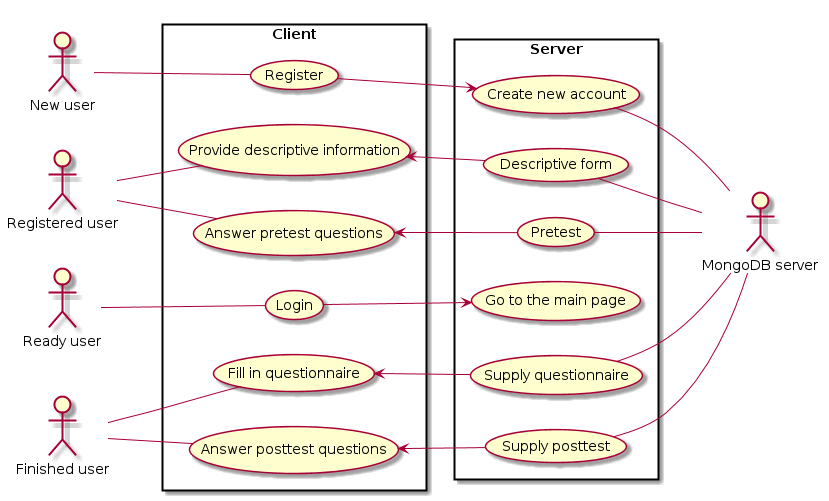
\includegraphics[width=\textwidth]{img/loginusecase.png}
\caption{An UML use case diagram for registering as new users or logging in as existing users}
\label{fig:loginusecase}
\end{figure}

\paragraph{Login use cases} When opening the webapplication, the user is first prompted with a login screen. Here, the user can either enter an already existing username to continue this session, or he can enter a new name in order to register as a new user. When the user is registering as a new user, a form is presented asking for information on gender and birthdate as descriptive information, and asking for the specific code the user received on the informed consent form in order to validate that the user indeed signed this form before partaking in the research (see section \nameref{sec:procedure} on page~\pageref{sec:procedure}). After that, another form will be prompted for the pretest (section \nameref{sec:instrumentation} on page~\pageref{sec:instrumentation}). When the user has met certain criteria, a posttest similar to the pretest will be prompted, followed by a questionnaire and a debriefing text. When none of these criteria are met, the user can access he main use cases.

\begin{figure}[h!]
\centering
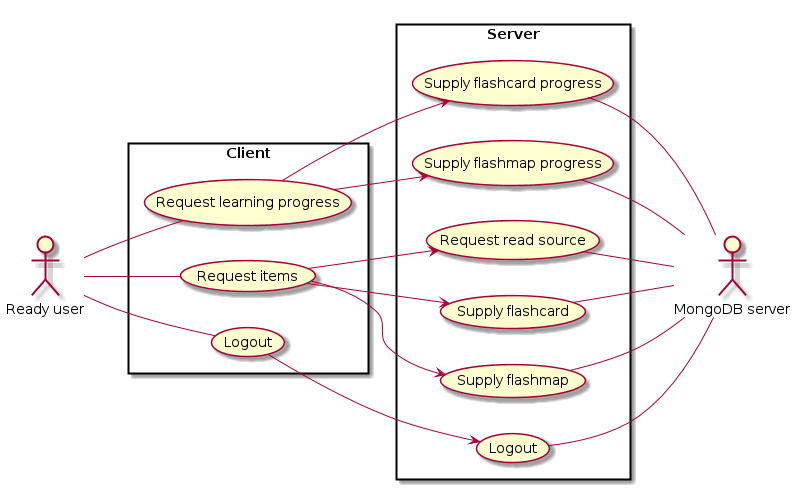
\includegraphics[width=\textwidth]{img/mainusecase.png}
\caption{An UML use case diagram for main uses of the application}
\label{fig:mainusecase}
\end{figure}

\paragraph{Learning use cases} The main use cases entail requesting items for review, requesting the learning progress, or logging out. When requesting items for review, the user can receive a due or new flashcard or flashmap, depending whether there are any old items due for review and the experimental group the user is in. Alternatively, the user can also be prompted whether a certain section of the instruction material has been read, since the rehearsal of items cannot be meaningful when the user is not familiar with the content. These prompts take often place at the beginning of a session so that the user does not have to interrupt a session. Furthermore, they prompt two sections ahead of the material currently being learned or reviewed by the user from the flashmap or flashcards in order to guarantee that the user is familiar with the material before learning the items. The user is prompted to read a section at most once per day. After the user has submitted a response, he can undo this response if he is not content with it. For example, the user could after seeing the correct response decide that he thought of a similar enough answer, but after deeper reflection still decide that his answer was not sufficient. In this case, he could use the undo option in order to be presented with the previous response again and select the 'incorrect' option.

\paragraph{Learning progress} When requesting the learning progress, the user is presented of an overview of what has already been learned and what is still left as either unseen items or items due for review. This provides an indication for the user so that he can estimate how much time he still needs to invest into the software, but also could stimulate the user by seeing the number of new or due items lowering and learned items increasing.

Finally, the user can return to the login screen by logging out.
 %Outlined
    \input{./design/scheduling.tex} %Not started
    \input{./design/visualisation.tex} %Not started
    \chapter{Software design and development}
\label{ch:software}

Within this chapter, the software is described from a user's perspective and linked to the design implications provided in the \nameref{ch:analysis} and the \nameref{ch:frameworks} chapters. The software is implemented as a webapplication in order to facilitate easy access from any webbrowser with internet connectivity. For a more technical description of the server and client, the full server documentation is included within the Flashmap Server Documentation appendix on page~\pageref{app:documentation}, and the client source code within the \nameref{app:clientsource} appendix on page~\pageref{app:clientsource}. Finally, the complete source code is available on github\footnote{\url{https://github.com/mcvdenk/MasterThesis-Software}}.

\section{Page elements}

Each page is represented as a webpage containing 4 different page elements, which are the navigation menu, the instructions panel, the main viewer, and a button panel. Within the different views of the application, they generally preserve the same functionality and layout, and will be explained below after the description of the colour scheme.

\subsection{Navigation menu}

The navigation is centered at the top of the screen, displaying buttons for the pages of the applications and a button to contact the developer for help (see figure~\ref{fig:navmenu}).

\begin{figure}
    \centering
    
\includegraphics[width=.8\textwidth]{img/navmenu.png}
    \caption{The navigation menu}
    \label{fig:navmenu}
\end{figure}

\subsection{Instructions panel}

The instructions panel is the next element is placed below the navigation menu, and is reserved for providing the user with extra instructions where needed. It does not have a background colour, but it does have a fixed height in order to keep all elements at the same place independent of the length of the instruction.

\subsection{Main viewer}

The main viewer is the central element, and expands from the instruction panel to the button panel. Within this container, the main content of the specific view is displayed, such as the flashcard or concept map, the questionnaire, or the login form. In order to stand out from the rest of the page, it has a separate background with rounded corners. The background colour is somewhat lighter in comparison to the general background colour in order for the text to be better readable. The main viewer is also the container for visjs, which is a javascript library for rendering graphs in browsers.

\paragraph{Visjs} Since the content contained within the graph is dynamic because of the partial maps returned from the server, generated automatic layouts of graphs are necessary. Visjs is capable of two models for automatic layout, namely hierarchical and force-directed. As described in the \nameref{sec:cmapframework} section on page~\pageref{sec:cmapframework}, the initial idea was to render the graphs as hierarchical. Upon trying this with different subgraphs however it was found that automatic assignment for the different nodes on different hierarchical levels was not correctly done by visjs. This is mainly due to the two options for hierarchical layouts, namely hubcentered and directed. The idea of a hubcentered hierarchy is that the levels of the nodes within the hierarchy are based on the amount of other nodes directly or indirectly linked to this node. This works especially well for tree graphs, but a concept map is not a tree graph because of the cross-links. The other option, directed hierarchy, should make advantage of the directed edges by determining the levels of the nodes based on the direction of the edges. Unfortunately, this is implemented within visjs as only the root and the leaves being determined whether there are only incoming or outgoing edges, whereas the rest of the nodes are still placed based on the hubcentered layout, unlike in other graph layout engines such as DOT. 

Because this rendering leads to more confusing graphs, the force-directed layout was chosen instead, despite this resulting in a more cyclical graphs common in other visualisation techniques such as mind maps. This layout engine attempts to position the nodes in such a way that all edges are about equally long and there are as few crossing edges as possible. This is done by assigning forces among the set of edges and the set of nodes, for example for having all nodes an inverse gravity force and all edges a spring force.

The other settings in visjs include options for assigning colours fitting within the existing colour scheme, and for the user being able to reposition nodes if for example the edge labels are not readable because of overlapping with other edges.

\subsection{Button panel}

Finally, within the footer of the page, a button panel is included. Here the user can choose to for example show the correct answer to a flashcard, or confirm that he has read a certain section within the instructional material. The layout of this panel is exactly the same as that of the navigation menu.

\section{Learning process}
\label{sec:client_learning}

The core functionality of the client is reviewing the user instances. In general, every time an instance is reviewed, first the question or incomplete flashmap is prompted, the user thinks of the correct answer, the client shows the correct answer, and finally the user indicates whether his answer was correct or incorrect. Alternatively, the system can prompt whether the user has read a certain section from the textbook, indicate that the user is finished with learning for today, or state that there are no more instances left to review. Finally, the user can also undo his last submitted response. These use cases are elaborated below.

\subsection{Read source}

Every time the user is encountered with a flashcard or flashmap from a new section within the instructional material, the user is prompted whether this section has been read, since the rehearsal of items cannot be meaningful when the user is not familiar with the content. These prompts take often place at the beginning of a session so that the user does not have to interrupt a session. Furthermore, they prompt two sections ahead of the material currently being learned or reviewed by the user from the flashmap or flashcards in order to guarantee that the user is familiar with the material before learning the items. The user is prompted to read a section at most once per day. Within the main viewer the question "Did you read section 13.1 already? If no, read this now." is displayed in Dutch. The user can then press the "Read" button in the button panel, which will lead to prompting the first instance. This screen is simular for each subsequent section prompt.

\begin{figure}
    \centering
    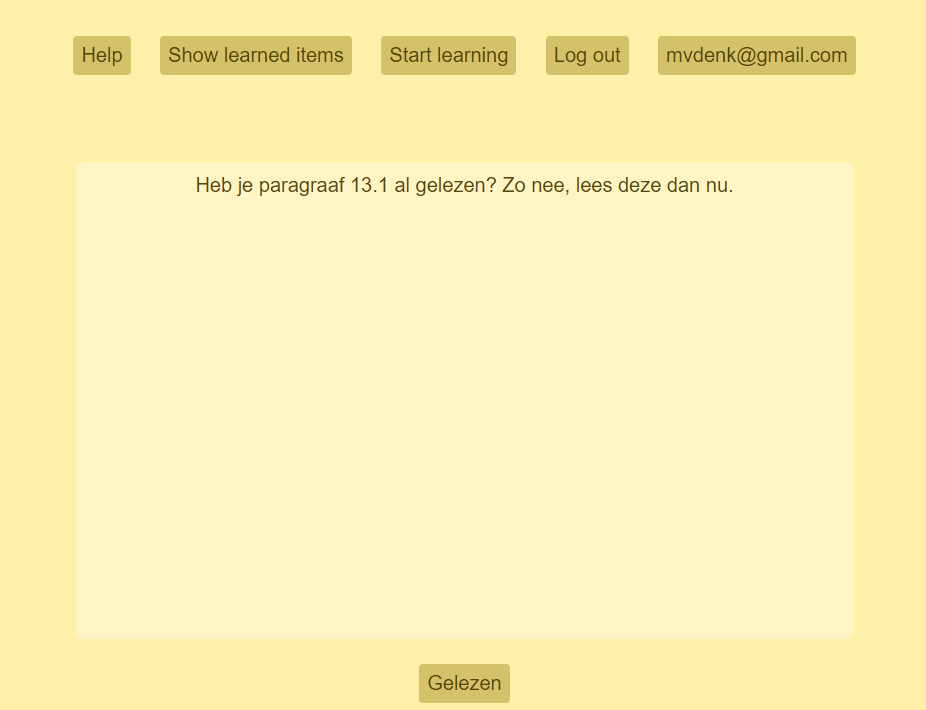
\includegraphics[width=.8\textwidth]{img/ui_read_request.png}
    \caption{The user interface when prompting the user whether he has read paragraph 13.1}
    \label{fig:ui_read_request}
\end{figure}

\subsection{Prompt}

When requesting items for review, the user can receive a due or new flashcard or flashmap, depending whether there are any old items due for review and the experimental group the user is in. If the user is a flashcard user, he will see the prompt such as in figure~\ref{fig:ui_fc_prompt}. The main viewer contains the specific flashcard question, and the button panel contains a button with the label "Show answer". The flashmap users get to see a partial incomplete flashmap within the main viewer (figure~\ref{fig:ui_fm_prompt}), which they can drag around and zoom in and out on. The cues which have to be retrieved are indicated by orange empty nodes.

\begin{figure}
    \centering
    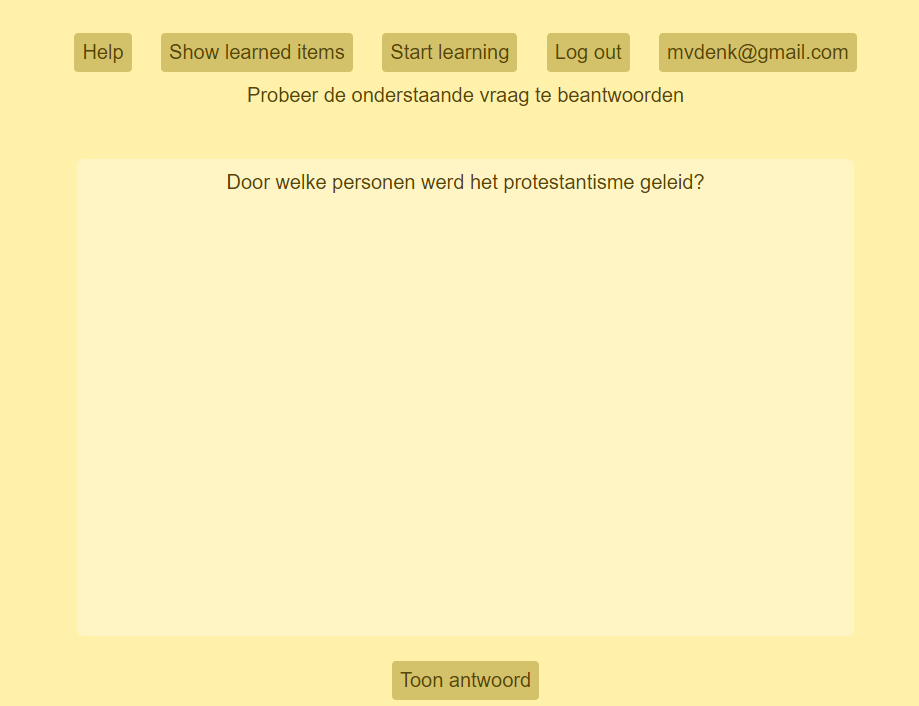
\includegraphics[width=.8\textwidth]{img/ui_fc_prompt.png}
    \caption{The user interface when prompting a flashcard}
    \label{fig:ui_fc_prompt}
\end{figure}

The partial map displayed to the user is a concept map containing all the concepts and relations which directly or indirectly point towards the relation which has to be learned (the parents), plus the concepts and relations linked to by the direct parent concept (the siblings). The reason why the parent concepts are returned rather than the child concepts is that in the instructional material the concepts are introduced top-down rather than bottom up, so building up the concept map from parent to child alligns better with the order in which the students read about the concepts. Additionally, the sibling nodes are also returned so that they can be prompted at the same time, and that the user has more context for deciding which concept should be filled in the missing node.

\begin{figure}
    \centering
    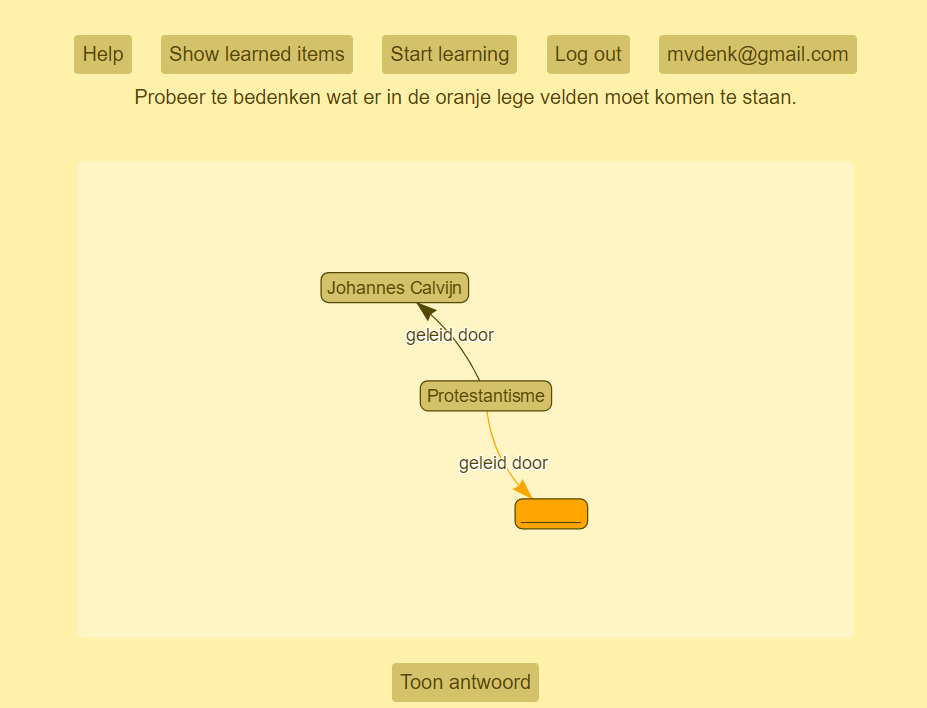
\includegraphics[width=.8\textwidth]{img/ui_fm_prompt.png}
    \caption{The user interface when prompting a flashmap}
    \label{fig:ui_fm_prompt}
\end{figure}

The button panel is the same for both conditions. The instructions element also shows instructions on what the user should achieve (to retrieve the correct answer from memory).

\subsection{Show answer}

After the user has pressed the "Show answer" button, the show answer prompt will be shown. Flashcard users get to see the correct answer in the main viewer below the question, with "Incorrect" and "Correct" buttons in the button panel to indicate whether the correct answer could be retrieved (figure~\ref{fig:ui_fc_answer}. Flashmap users get to see the correct answers within the previously empty nodes, which will also turn green indicating that the user retrieved them correctly (figure~\ref{fig:ui_fm_answer_correct}). When the user did not retrieve an answer correctly, he can click on that node, turning it red (figure~\ref{fig:ui_fm_answer_incorrect}). After the user indicated the correct and incorrect retrievals, he can click on a "Next" button in the button panel. The instructions element again contains instructions on what to do within this screen.

When the user has submitted at least one response within one session, he can undo this response if he is not content with it. For example, the user could after seeing the correct response decide that he thought of a similar enough answer, but after deeper reflection still decide that his answer was not sufficient. In this case, he could use the undo option in order to be presented with the previous response again and select the 'incorrect' option. The "Undo" button appears left to the "Show answer" button (see figure~\ref{fig:ui_undo}).

\begin{figure}
    \centering
    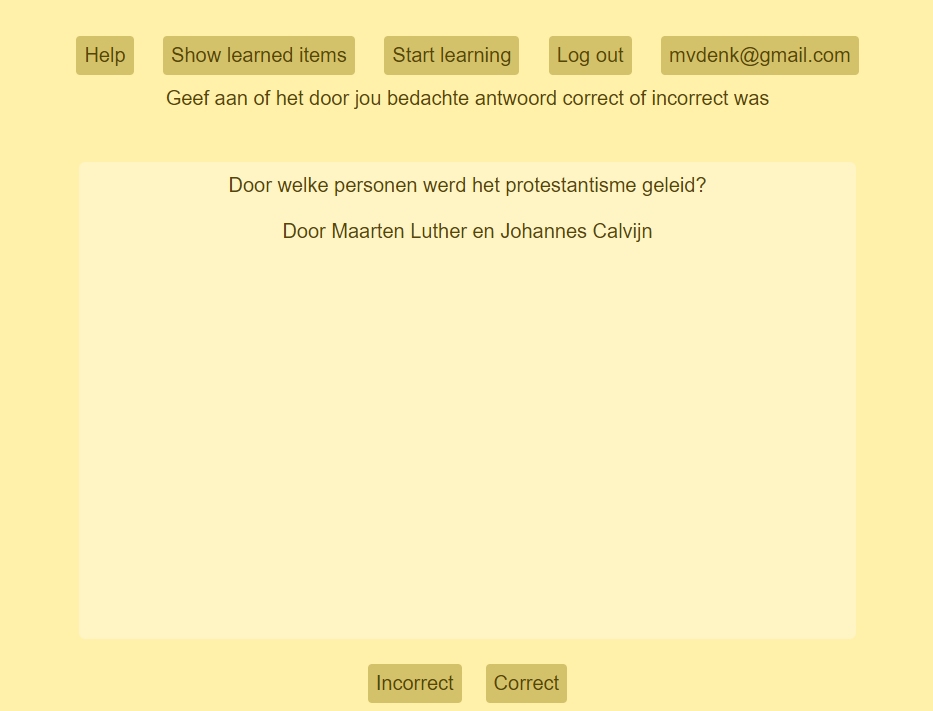
\includegraphics[width=.8\textwidth]{img/ui_fc_answer.png}
    \caption{The user interface when showing the answer to a flashcard}
    \label{fig:ui_fc_answer}
\end{figure}

\begin{figure}
    \centering
    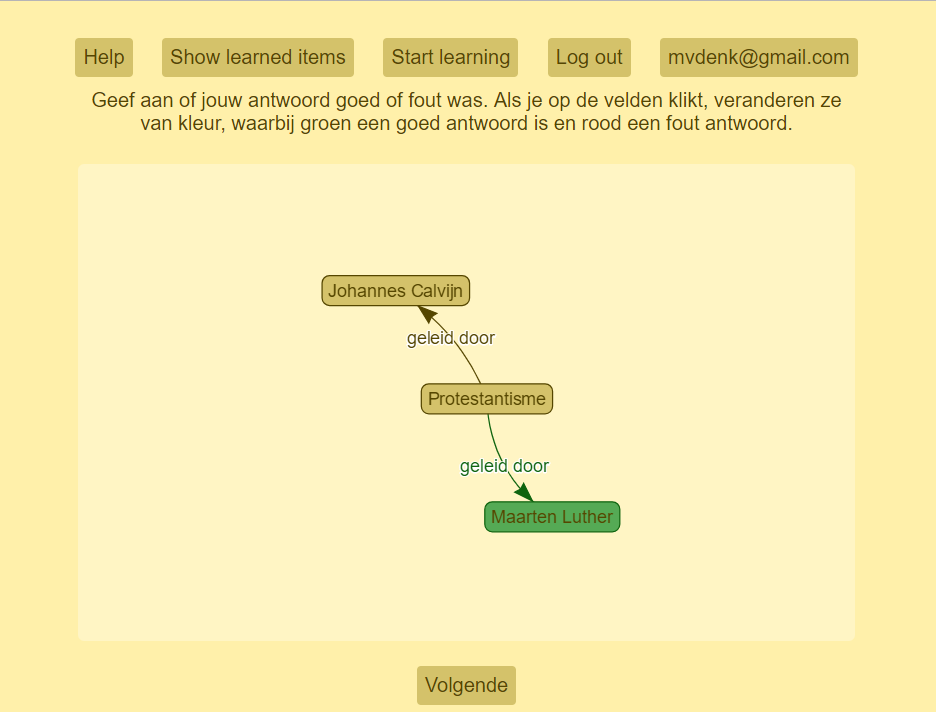
\includegraphics[width=.8\textwidth]{img/ui_fm_answer_correct.png}
    \caption{The user interface when showing the answer to a flashmap, here indicated as correct by the user}
    \label{fig:ui_fm_answer_correct}
\end{figure}

\begin{figure}
    \centering
    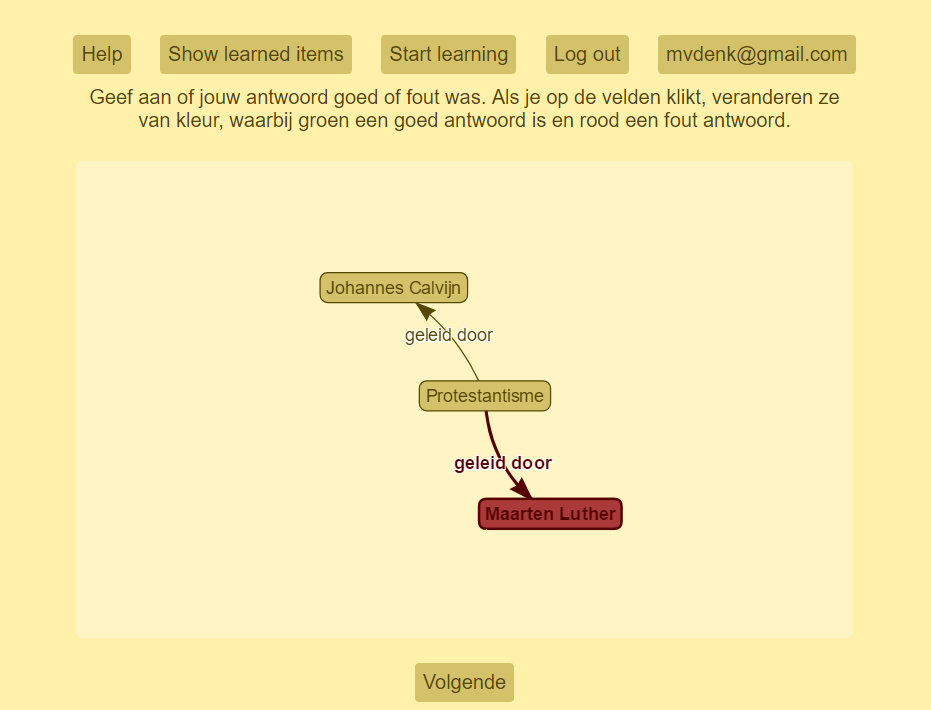
\includegraphics[width=.8\textwidth]{img/ui_fm_answer_incorrect.png}
    \caption{The user interface when showing the answer to a flashmap, here indicated as incorrect by the user}
    \label{fig:ui_fm_answer_incorrect}
\end{figure}

\begin{figure}
    \centering
    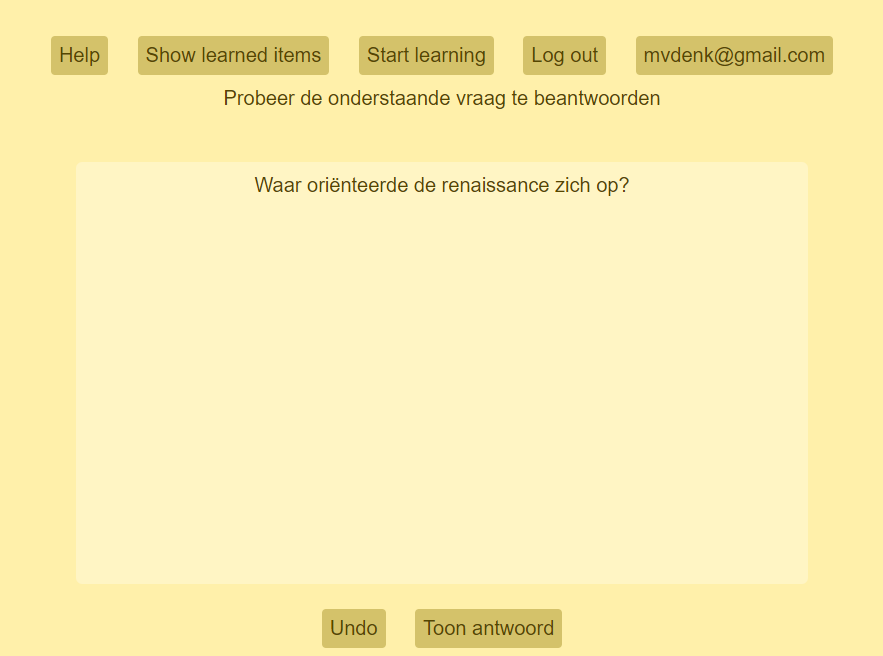
\includegraphics[width=.8\textwidth]{img/ui_undo.png}
    \caption{The user interface when prompting a flashcard with an undo option}
    \label{fig:ui_undo}
\end{figure}

After the user has provided the answer to the system, the system reschedules the flashmap or flashcard. In the~\nameref{subsec:adaptivesequencing} chapter on page~\pageref{subsec:adaptivesequencing}, it is described that in order to calculate the interval until the next review, one needs the number of correct responses since the last incorrect response. This is done by going through all the responses for the specific flashcard or flashmap in descending order of sent in date, increasing a counter until an incorrect response is found. Then, $5^{exp}$ seconds are taken as the interval until the next review of the flashcard or flashmap. Examples:
%
\begin{itemize}
    \item When there are no responses, the interval is $5^{1+0}=5$ seconds;
        \item When there are two correct responses, the interval is $5^{1+2}=125$ seconds;
        \item When there are two correct responses, followed by one incorrect response and then three correct responses, the interval is $5^{1+3}=625$ seconds.
\end{itemize}

\begin{figure}
\centering
    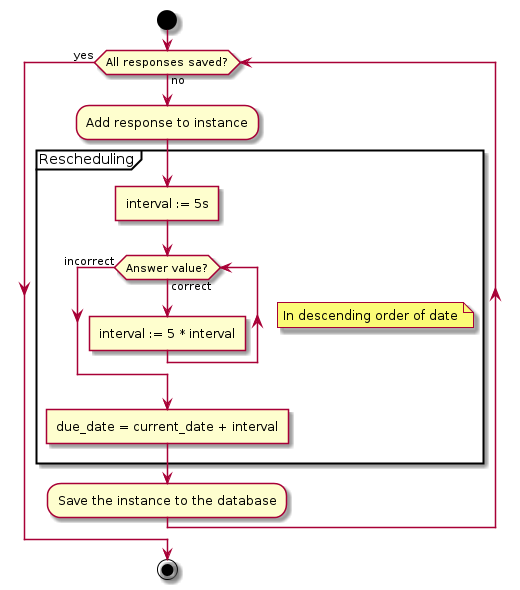
\includegraphics[height=.5\textheight]{img/learningserver.png}
\caption{An UML activity diagram showing the scheduling and saving of a list of responses within instances}
\label{fig:learningserver}
\end{figure}

\subsection{Finished learning and No more instances}

Finally, when the user has spent 15 minutes on the system or when there are no instances left to review, the user gets to see a screen such as in figure~\ref{fig:ui_no_more_instances}. The main viewer contains information on why the user is finished. When the user is finished because there are no more instances left in the sections he already read but there are still instances available in following sections, it also shows which section the user could read for the next instance, and presents a button to continue. Finally, if the user spent 6 days on the system, this prompt will also inform him that the next day he can take the posttest and fill in the questionnaire.

\begin{figure}
    \centering
    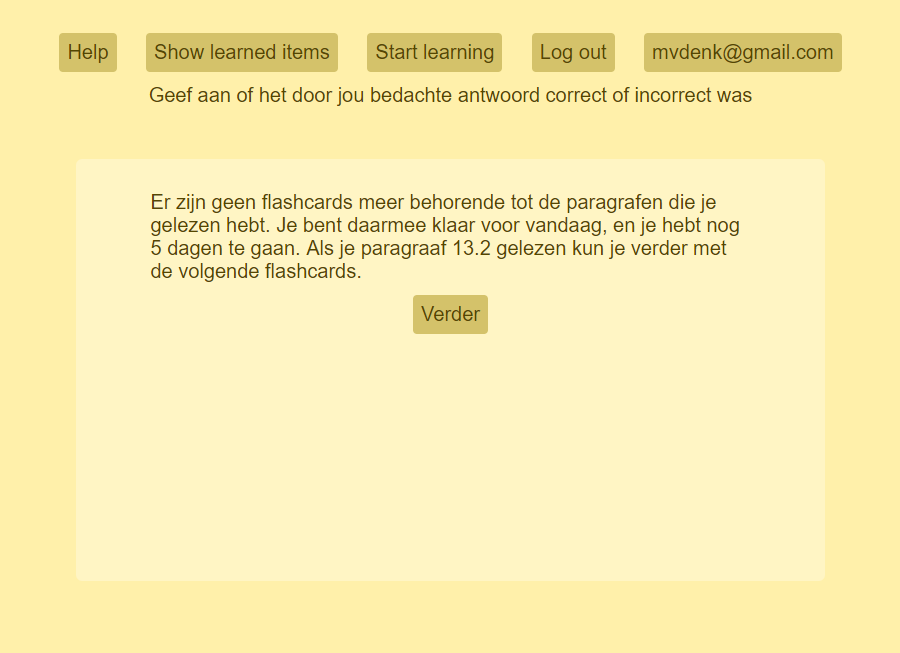
\includegraphics[width=.8\textwidth]{img/ui_no_more_instances.png}
    \caption{The user interface when showing that there are no new instances left to learn}
    \label{fig:ui_no_more_instances}
\end{figure}

\section{Other views}

Next to the main functionality described in the previous section there are also other views for accommodating the other use cases. For new users, these are the login screen, the descriptives screen, and the pretest, for regular users there are the help screen and the learning progress screen, and for the users which are finished there are the posttest, questionnaire, and debriefing screens.

\subsection{Login screen}

The main viewer in the login screen containing a simple form with a textfield for the username, and a submit button for logging in (figure~\ref{fig:ui_login}). Furthermore, a text within the instructions panel refers the users to the researcher's email adress for when they require further instructions or when the logging in does not function.

\begin{figure}
    \centering
    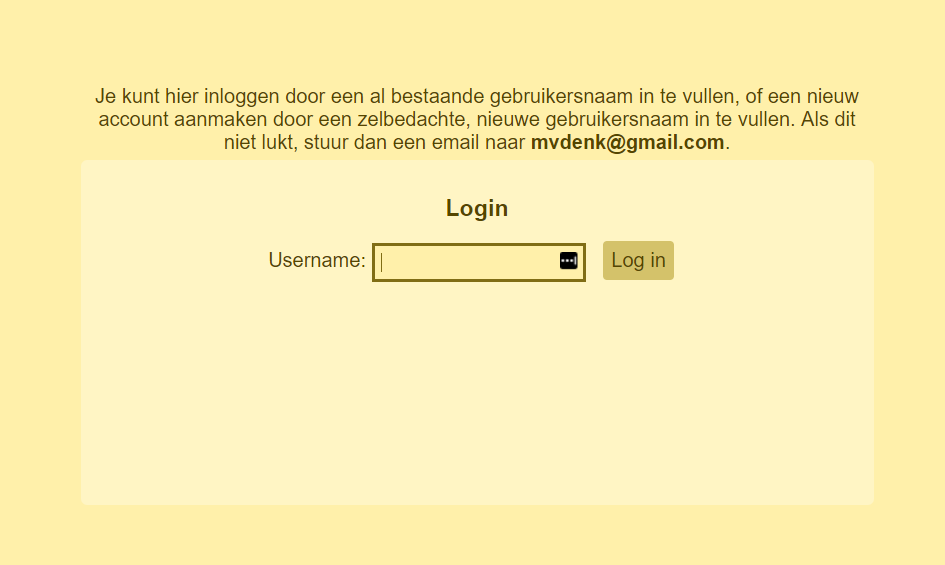
\includegraphics[width=.8\textwidth]{img/ui_login.png}
    \caption{The login screen}
    \label{fig:ui_login}
\end{figure}

\subsection{Descriptives, Test and Questionnaire forms}

These screens also contain basic forms, all containing questions or items and either textfields or radiobutton selection panels, depending on whether the question or item is open or closed, and a submit button at the bottom. (figures~\ref{fig:ui_descriptives}, \ref{fig:ui_test}, and~\ref{fig:ui_questionnaire}). The date field within the descriptives form is checked to be a valid date before the user can submit. Furthermore, the questionnaire item contains an email field for when the user wants to sign up for a later interview, which is a voluntary field and can be left empty. The instructions element again provide instructions for how to fill in the forms.

\begin{figure}
    \centering
    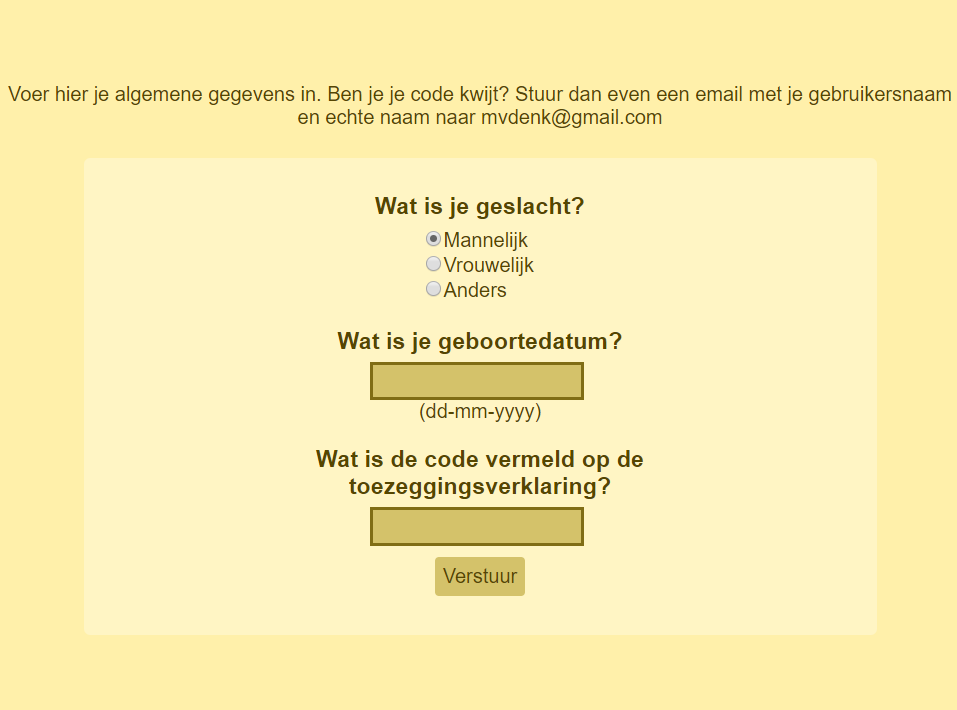
\includegraphics[width=.8\textwidth]{img/ui_descriptives.png}
    \caption{The descriptives screen}
    \label{fig:ui_descriptives}
\end{figure}

\begin{figure}
    \begin{subfigure}{0.4\textwidth}
        \centering
        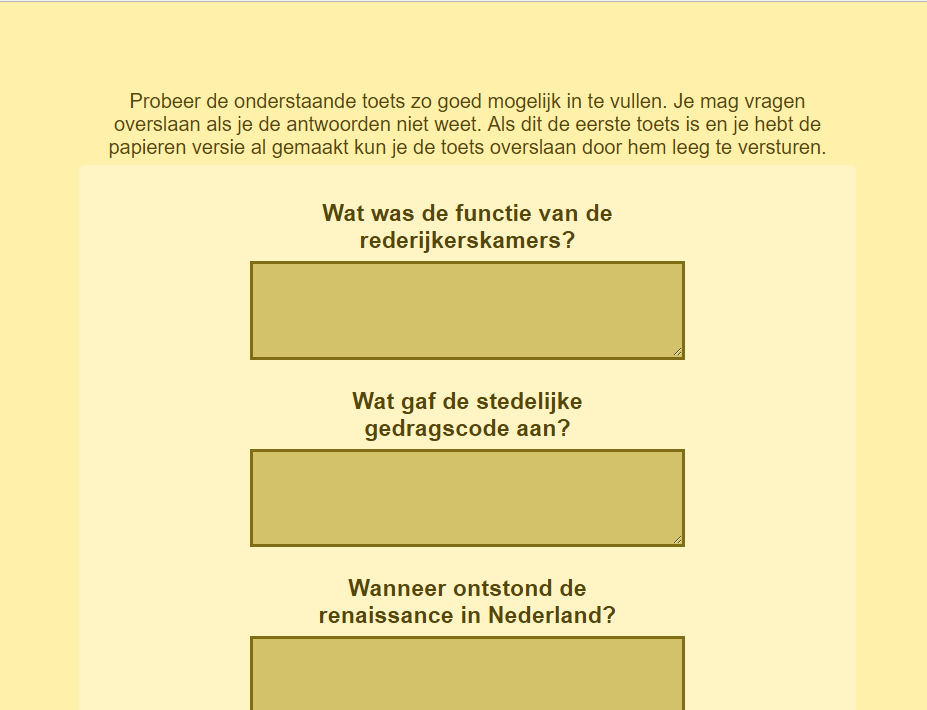
\includegraphics[width=\textwidth]{img/ui_test_top.png}
        \caption{Top}
        \label{fig:ui_test_top}
    \end{subfigure}
    \qquad
    \begin{subfigure}{0.4\textwidth}
        \centering
        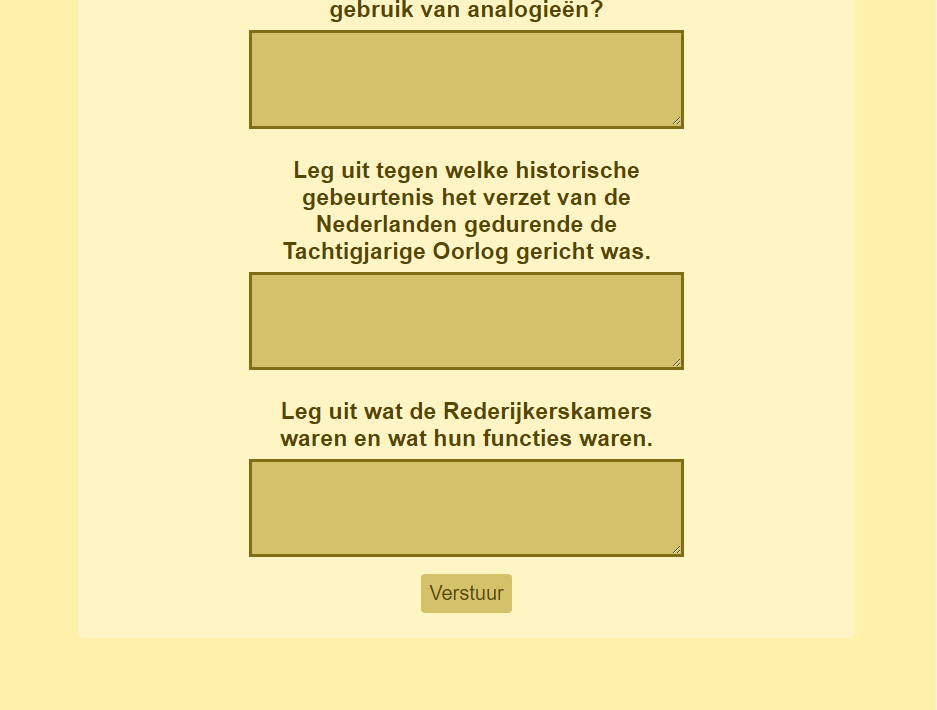
\includegraphics[width=\textwidth]{img/ui_test_bottom.png}
        \caption{Bottom}
        \label{fig:ui_test_bottom}
    \end{subfigure}
    \caption{The test screen}
    \label{fig:ui_test}
\end{figure}

\begin{figure}
    \begin{subfigure}{0.4\textwidth}
        \centering
        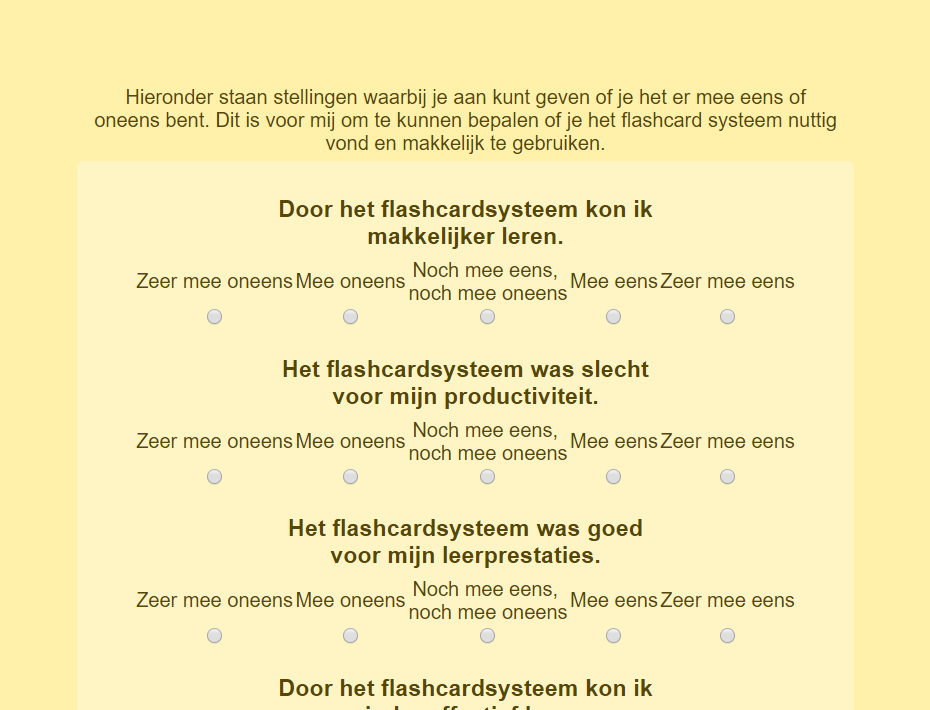
\includegraphics[width=\textwidth]{img/ui_questionnaire_top.png}
        \caption{Top}
        \label{fig:ui_questionnaire_top}
    \end{subfigure}
    \qquad
    \begin{subfigure}{0.4\textwidth}
        \centering
        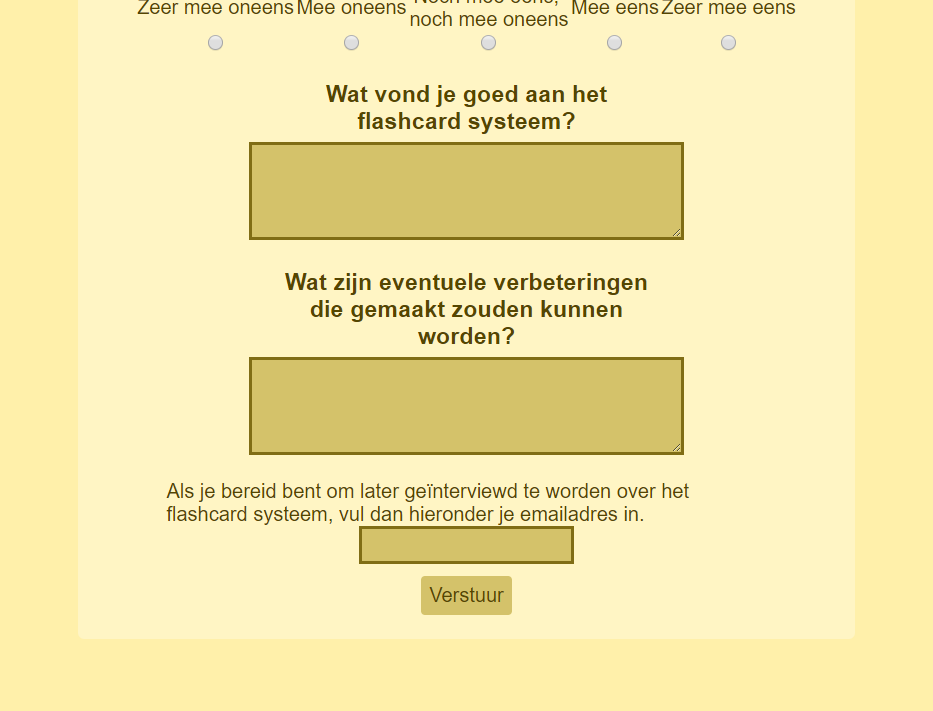
\includegraphics[width=\textwidth]{img/ui_questionnaire_bottom.png}
        \caption{Bottom}
        \label{fig:ui_questionnaire_bottom}
    \end{subfigure}
    \caption{The questionnaire screen}
    \label{fig:ui_questionnaire}
\end{figure}

\subsection{Debriefing}

Finally, when the user is finished using the system and filling in the posttest and questionnaire, the application presents the debriefing information (figure~\ref{fig:ui_debriefing}). This entails a thank you message, that the user will receive the coupon for ice cream soon, that he is able to keep using the system, that he can request his personal data gathered during the experiment from the researcher at any time, that he will receive an email for making an appointment for the interview when he filled in his email address, and that for further questions he can always send an email to the researcher's email address. When the user has read this information he can click the "Read" button.

\begin{figure}
    \centering
    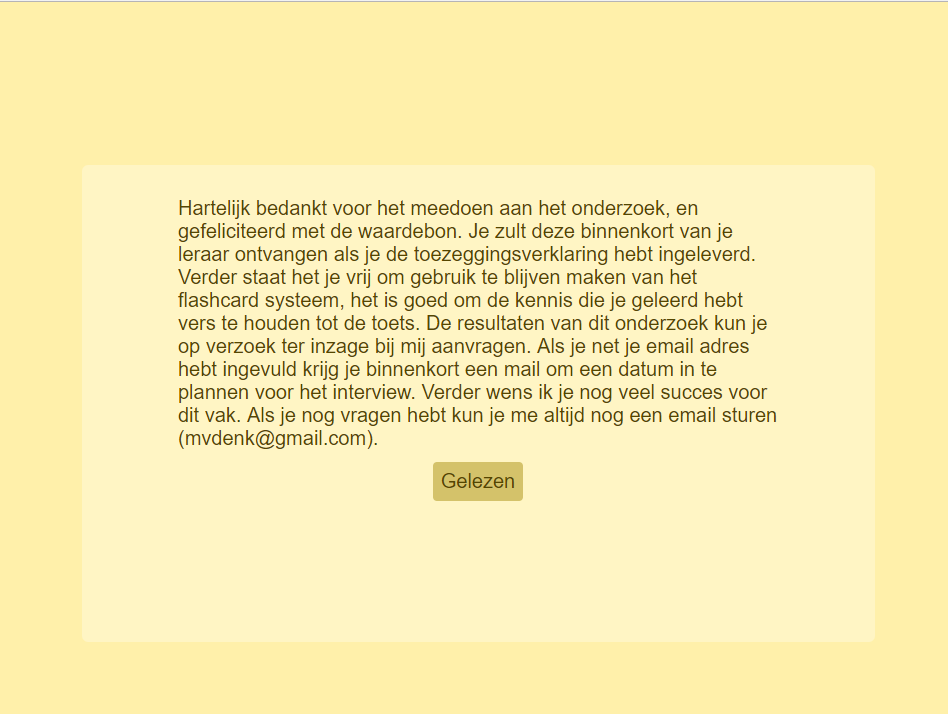
\includegraphics[width=.8\textwidth]{img/ui_debriefing.png}
    \caption{The debriefing screen}
    \label{fig:ui_debriefing}
\end{figure}

\subsection{Help}

The help screen (figure~\ref{fig:ui_help}) contains some global information about the experiment and on what conditions the user can receive the icecream coupon. It also states that the system will notify the user as soon as he is ready for today.

\begin{figure}
    \centering
    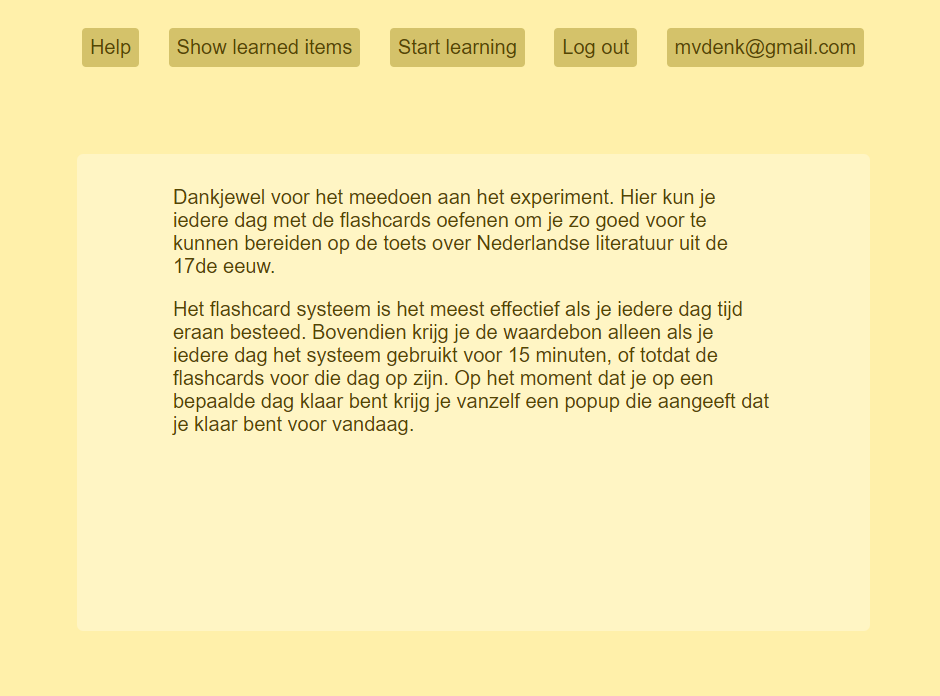
\includegraphics[width=.8\textwidth]{img/ui_help.png}
    \caption{The help screen}
    \label{fig:ui_help}
\end{figure}

\subsection{Learning progress}
\label{sec:learningprogress}

Finally, the user can request information about how much progress he made. Flashcard users are presented with how many cards are ready to be learned right now, how many are never reviewed, how many are new (less than exponent 2), how many are in the learning stage (less than exponent 6) and finally how many cards have been learned for the long term (more than exponent 6). Figure~\ref{fig:ui_fc_learnprogress_1} shows a learning progress screen of a new flashcard user, and figure~\ref{fig:ui_fc_learnprogress_2} an shows this overview for a user having correctly reviewed one flashcard but incorrectly reviewed another flashcard. The flashmap user is shown with a different overview, namely the part of the concept map containing the edges already reviewed by the user (figure~\ref{fig:ui_fm_learnprogress}), which will expand during the use of the system.

These views can still be improved in order to better convey the progress towards a user, which would contribute to a higher self-reinforcement. However, this has not yet been implemented due to time constraints.

\begin{figure}
    \begin{subfigure}{0.4\textwidth}
        \centering
        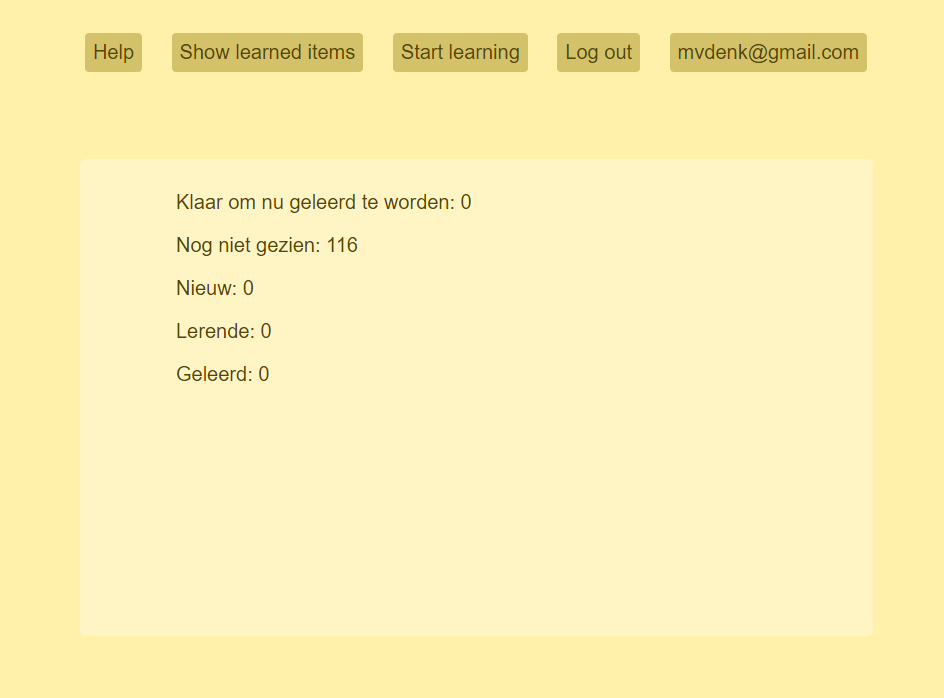
\includegraphics[width=.8\textwidth]{img/ui_fc_learnprogress_1.png}
        \caption{For a new flashcard user}
        \label{fig:ui_fc_learnprogress_1}
    \end{subfigure}
    \qquad
    \begin{subfigure}{0.4\textwidth}
        \centering
        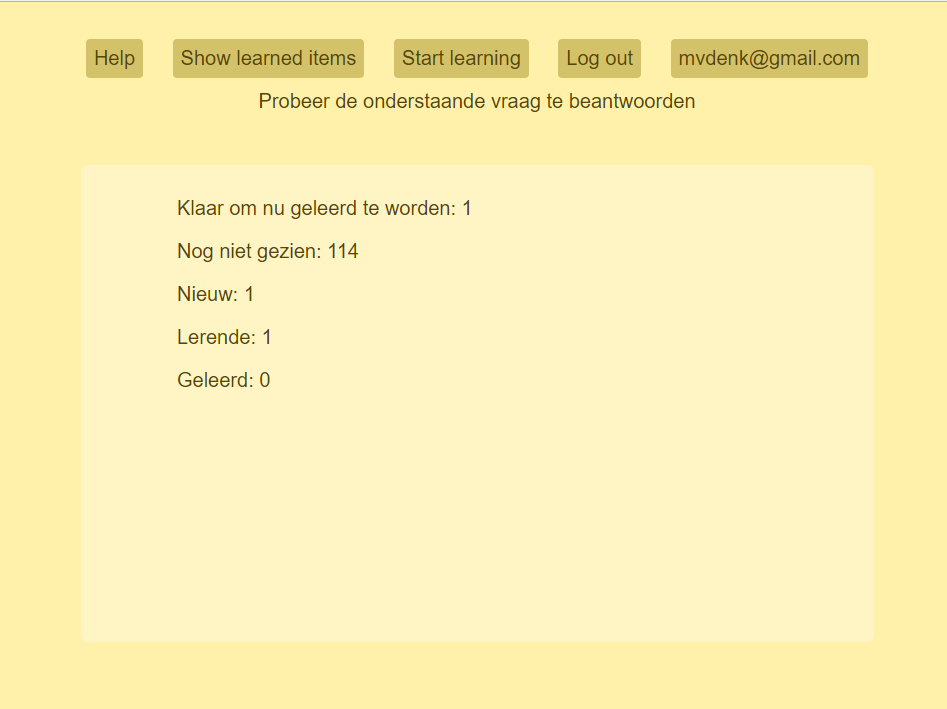
\includegraphics[width=.8\textwidth]{img/ui_fc_learnprogress_2.png}
        \caption{For a flashcard user having reviewed some flashcards}
        \label{fig:ui_fc_learnprogress_2}
    \end{subfigure}
    \caption{The user interface when showing the learning progress to a flashcard user}
    \label{fig:ui_fc_learnprogress}
\end{figure}

\begin{figure}
    \centering
    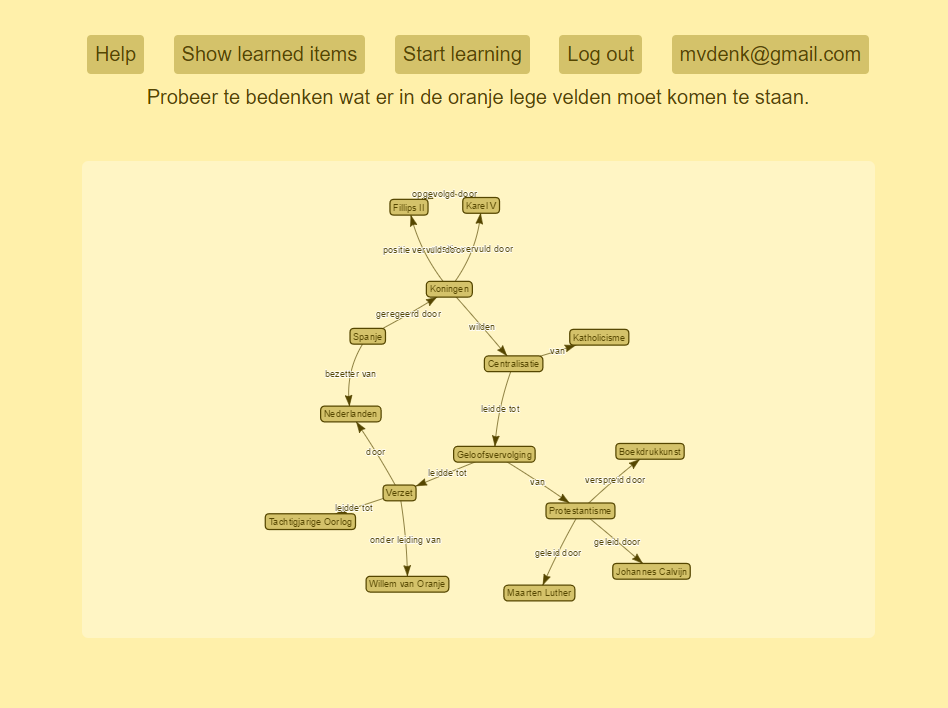
\includegraphics[width=.8\textwidth]{img/ui_fm_learnprogress.png}
    \caption{The user interface when showing the learning progress to a flashmap user}
    \label{fig:ui_fm_learnprogress}
\end{figure}

\section{Testing the software}

All of the above described functions are tested thoroughly using unittests (\url{https://github.com/mcvdenk/MasterThesis-Software/tree/master/server/unittest}) and using black-box tests from within the client.
 %Not started

\part{Research}
    \chapter{Aims and goals for the research}
\label{ch:aimsgoals}
 %Not started
    \chapter{Methods}
\label{ch:methods}

\section{Research design}
\label{sec:researchdesign}

Research questions~\ref{benefit}\ref{effectiveness}, \ref{efficiency}, \ref{perception}\ref{usefulness} and \ref{ease} will be investigated using intervention-based research. Because of the systems being used for self-study by the students, they can be individually assigned to a condition, and this enables the use of a true experimental design. Since this will provide the most valid and reliable results, this research design is implemented in this experiment.

Additionally, research questions~\ref{usefulness} and \ref{ease} will also be investigated using open questions on the questionnaire form and by conducting interviews with a sample of the participants.

Finally, research question~\ref{howused} will be investigating both quantitatively by logging the user behaviour during the experiment and by the open questions and interviews also used for research questions~\ref{usefulness} and \ref{ease}.

The quantitative and qualitative results will be mixed for the purposes of triangulation and expansion as described by \citeA{mixedmethods}. The interviews and logs could provide insight in the degree of which the systems were used the intended way and in why students had certain perceptions on using the systems. Both triangulation and expansion will be on a partial level of mixing, will take place concurrently, and the quantitative data will be dominant, since the qualitative data exists only to triangulate and expand the quantitative data. 

\section{Respondents}
\label{sec:respondents}

100 15 to 17 year old tenth grade Dutch high school students will be approached. They already have to prepare themselves for an exam on the same topic and thereby have incentive to learn. To increase the response rate, the students will be rewarded with a \euro{} 5 voucher for participation. The participants will be assigned to either the flashcard or the flashmap condition at random when they create a user account within the webapplication.

\section{Procedure}
\label{sec:procedure}

\paragraph{Review concept map, flashcards, and item bank} In order to verify whether the content offered within the system is in alignment with the learning goals set by the teachers, one of the teachers is asked to review the content. The feedback received from the teacher is afterwards incorporated by altering the dataset. This can be seen as the focus evaluation of the product \cite{slo}.

\paragraph{Approval ethical committee} Before the actual experiment can take place, the research setup first has to be approved by the ethical committee of the University of Twente. This takes place before the system is introduced to the students.

\paragraph{Presentation} Within the school curriculum there are two instructions planned for the topic of Dutch renaissance literature. At the end of the instruction, the researcher introduces the experiment and the system to the participants. This is meant both to attract students to participate, but also to provide a briefing next to the written briefing. Within the presentation, the benefits are stated (better preparation for the exam, preview for the exam), it is stressed that participation is voluntary and that the data will be collected anonymously, the informed consent form will be introduced, and finally the reward (icecream vourchers) will be announced, together with the conditions for receiving the reward.

\paragraph{Informed consent form} The informed consent form, included within the \nameref{app:consentform} appendix on page~\pageref{app:consentform}, contains a letter, the written briefing, and a form which has to be signed by both the parent or caretaker and the participant. It also contains a code with which it can be verified that a user within the system did indeed sign this form. The briefing contains a description of the research, the advantages of participation, and the procedure of the experiment.

\paragraph{Division of respondents} Users will be assigned alternately to the control group or the experimental group. This pseudo-random assignment increases the validity of the experimental design without risking one group becoming larger than the other group. This however only holds up for the initial group, because dropout rates between the group could vary resulting in differently sized finished groups.

\paragraph{Descriptives} Before the experiment itself starts, the gender and the birthdate of the participants are prompted. This provides descriptive statistics necessary for the measure of generalisability of the results.

\paragraph{Pretest} Another form prompted towards the user before the start of the experiment is the pretest, measuring how much the user already knows and understands about the subject. This test is elaborated within the next section.

\paragraph{Experiment} The experiment itself consists of the participants having to review instances for 15 minutes over the course of 6 days. The 15 minutes are estimated to be the amount of time necessary to review one section in the instructional material, and the 6 days are chosen as a balance between having covered a large enough portion of the material to measure a significant learning gain without the participant investment being too large resulting in no student wanting to participate. The 6 days of learning ideally take place subsequently, since then students have a higher chance of retrieving repeating instances correctly. However, it is likely that participants could forget about the experiment or be too busy to invest the 15 minutes, and therefore they are allowed one non active day during the experiment. Each session consists of being presented by questions or incomplete concept maps, trying to retrieve the correct answer or missing concepts from memory, and indicating whether the correct answer or missing concept was successfully retrieved.

\paragraph{Posttest} The seventh day the participant logs in to the system he is prompted with the posttest in order to measure the level of knowledge and comprehension after the experiment. This test uses the same itembank as the pretest, and is thereby also elaborated within the next section.

\paragraph{Questionnaire} After filling in the posttest, the participant is also asked to fill in a questionnaire based on the Technology Acceptance Model, which is further elaborated within the next section. The form also contains two open questions, namely to describe what the participant thought was good about the system, and what he thought could be improved. Finally, he can fill in his email address if he is interested in being interviewed afterwards.

\paragraph{Debriefing} Finally, the participant is presented with the debriefing text from figure~\ref{fig:ui_debriefing} on page~\pageref{fig:ui_debriefing}. This states that the user will soon receive the voucher, that he is allowed to keep using the system, and that he can contact the researcher if he has questions or when he wants to see his personal data. The participant is now finished with the main experiment.

\paragraph{Scoring sample items} After all the results have been gathered, a small sample of the responses are reviewed by both one of the teachers and the researcher in order to establish an inter-rater reliability. This will take place after the school test itself, but before the teacher has scored the test administered by the school itself to remain unbiased. Furthermore, the sample will be a random anonymous selection of responses in order to minimise any halo effect. Finally, the samples are filtered on non-empty items which do also not exactly correspond to the response model, since these can be automatically scored. If the inter-rater reliability is too low, the scoring rubics will be altered in order to differentiate better among correct or incorrect responses, and the procedure is repeated. Otherwise, the rest of the responses is scored by the researcher.

\paragraph{Interview} Those who volunteered for the interview will be sent an invitation by email for a group interview. This format is chosen, since an email interview is obsolete because of the open questions on the questionnaire form, and individual interviews being infeasible because of a room within the school having to be reserved for a longer time.

\paragraph{Icecream vouchers} The vouchers and the list containing the names of students having participated within the experiment will be handed over to the students after the scoring of the test administered within the school in order to avoid influencing the teachers during the marking of the tests.

\section{Instrumentation}
\label{sec:instrumentation}

\subsection{Test}

\subsection{Questionnaire}

\subsection{Data collection during experiment}

\paragraph{Correctness retrievals}

\paragraph{Retrieval time}

\paragraph{Session data}

\paragraph{Log entries}

\subsection{Interview}

\section{Analysis}
\label{sec:analysis}

\paragraph{Inter-rater reliability}

\paragraph{Classical test theory}

\paragraph{Item response theory}

\paragraph{Learning gain}

%Absolute and relative

\paragraph{Instance statistics}

\paragraph{Questionnaire statistics}

\paragraph{Comparisons}

\paragraph{Hypotheses}

\paragraph{Interviews}
 %Not started
    \chapter{Results}
\label{ch:results}

\section{Participant descriptions}

\subsection{User participation}

The \nameref{app:participation} appendix on page~\pageref{app:participation} shows statistics on how many days the different used the system. In table~\ref{tab:participation_incl} it is shown that in total 63 students made an account within the system. From these students 44 used the system on at least one day for longer than 15 minutes, of which the average student participated on 4.68 days. These statistics are also summarised within figure~\ref{tab:participation}. The usage of the system is also depicted in figures~\ref{fig:participation} and~\ref{fig:participation_gen}. Finally, figures~\ref{fig:activedays_fc}, \ref{fig:activedays_fm}, and \ref{fig:activedays_gen} within the appendix display on which days users have been actively using the system as a scatter diagram, and how many users cummulatively have finished using the system as a step diagram, for the flashcard and flashmap seperately and the combined conditions, where day 0 is the day the system was introduced within the presentation and day 21 the final day before the exam.

Interesting to note here is that there are two subsequent strong increases in finished users around 6 days after the system was introduced, but that there is also a very strong increase the day before the students' exam. This is also reflected within a highly increased activity within the first week, and on the day before the exam. There is even some noticable activity after the exam took place, possibly of students already having invested some time into the system before the exam, but still finishing up in order to be rewarded with the icecream voucher. This resulted in a total number of 25 finished users, of which 13 users within the flashcard condition and 12 users within the flashmap condition. Both in the flashcard and the flashmap condition there is one user which did use the software for 6 days, but then did not partake in the posttest. Finally, in figure~\ref{fig:participation_gen} it can be seen that there are 4 students which used the system for only 5 days, which meant that they just missed out on the reward.

Within the interviews, it was gathered that students were mainly interested in participation, because they had problems preparing the previous exams from the same course and that they believed the system to help them being better prepared. The icecream voucher was only a secondary motivator, but a motivator nonetheless. One student indicated that the system might however be more successful within younger students, since the older students often already have their own learning systems and prefer to stick to these systems.

A sample of 23 divided over two conditions is too small for making any generalisations, and therefore any results stemming from this experiments are only indicatory and should be further investigated before they can be used. Since the only students usable for the rest of the result section are those finishing the posttest, the other students will be omitted from consideration.

\begin{table}
    \centering
    \begin{tabular}{lrrrrr}
        \toprule
        & $\mu_{fc}$ & $\mu_{fm}$ & $p$ \\
        \midrule
        Including zero days & 3.27 & 3.27 & 0.994 \\
        Excluding zero days & 4.32 & 5.16 & 0.984 \\
        \bottomrule
    \end{tabular}
    \caption{Compact view of the participation statistics for both all enrolled users and only including the users with at least one day of participation}
    \label{tab:participation}
\end{table}

\subsection{Descriptive variables}

The participant descriptives are included in the \nameref{app:descriptives} appendix on page~\ref{app:descriptives}, containing distributions of student gender and age.

\paragraph{Gender} As can be seen in figure~\ref{tab:gender}, 15 out of the 23 total participants are male and 8 are female, where within the flashcards condition there is a 7 to 5 ratio and within the flashmap a 8 to 3 ratio. This is probably just coincidental due to the small sample size.

\paragraph{Age} All students have an age within the range of 15 to 17 with an average age of 15.75 and a modus of 16, which is to be expected from VWO4 students. There is also no considerable age difference among the conditions, indicated in table~\ref{tab:age_comp} and figure~\ref{fig:age}.

\section{Learning gain}

The pre- and posttest statistics are displayed in the \nameref{app:learning_gain} appendix on page~\ref{app:learning_gain}, divided in the inter-rater reliablity statistics and the result scores on the test. 

The results are separately described for the knowledge questions and comprehension scores on the test, since they measure different variables. The different scores described and compared are the pretest scores, posttest scores, total scores, and the absolute (abs\_learn\_gain) and relative learning gains (rel\_learn\_gain). Additionally, they are reported as classical test theory scores (ctt), item response theory person abilities (irt), and person abilities from item response theory using fixed item difficulties from the combined pretest scores (fixed irt). Per category, the sample size, minimum, maximum, and mean values are displayed as descriptive values; the skew, kurtosis, and t and p values from the scipy normaltest are displayed as values for describing the distribution of the results; and $\alpha$ describes the reliability of the test (either Cronbach's alpha for the ctt results or the EAP value for the irt results). These results are described for the flashcard condition, the flashmap condition, and the combined sample of both conditions. The included graphs display histograms depicting the test matrices. Finally, the pre- and posttest scores are compared with each other by means of the non-parametric Mann-Whitney U test and the parametric Welchs' t-test in order to verify that users scored significantly higher on the posttest than on the pretest, and the learning gains between conditions are compared in order to answer research question~\ref{benefit}\ref{effectiveness}.

Remarkable are the low scores on the tests, with on average only 1.3 points on the knowledge questions (0.43 on the pretest and 2.17 on the posttest) and only 1.33 points on the comprehension questions (0.33 on the pretest and 2.33 on the posttest). This would indicate that the tests are exceptionally difficult, even though the questions are directly derived from the textbook itself and the users drilling these questions over the course of 6 days. Especially the low posttest knowledge question scores from the flashcard group are striking, since these questions were literally rehearsed during the experiment.

For both the knowledge questions as for the comprehension questions, the ctt reliability for the combined pre- and posttest score for the combined flashcard and flashmap users is around .7 --- mainly because the omission process of unreliable items ---, whereas the fixed irt reliability is around .6 (see table~\ref{tab:know_gen} and table~\ref{tab:comp_gen}). According to \citeA{devellis}, this means that the results obtained from classical testing are acceptable, whereas the results obtained from the item response theory are questionnable at best. Additionally, both the score outcomes, the figures, and the pre- and posttest comparisons in tables~\ref{tab:know_pp_fc_comp}, \ref{tab:know_pp_fm_comp}, \ref{tab:know_pp_gen_comp}, and tables~\ref{tab:comp_pp_fc_comp}, \ref{tab:comp_pp_fm_comp}, \ref{tab:comp_pp_gen_comp} indicate an average positive learning gain from the classical test theory, but a negative gain from the item response theory. Therefore, the conclusion will be based on the results from the classical test theory only.

Table~\ref{tab:learning_gain_effect} summarises the results related to learning gains. In the rows, the absolute and the relative classical test scores and the absolute item response theory person ability scores with fixed item difficulties are included for both the knowledge and comprehension questions. The item response theory results are only included for reference, and from this only the absolute learning gains are taken into consideration, since the person abilities are already estimated relative to the item difficulties. the columns include the reliability, the p-value of the normality test, the flashcard and flashmap mean score, and the p-values for in this case the Mann-Whitnney U test, since none of the results seem to be normaly distributed.

The flashmap users seem to have a higher learning gain than the flashcard users on the knowledge questions, and that looking at only the ctt results they seem to have a lower gain on the comprehension questions. None of the Mann-Whitney U test p-values for the ctt results seem to be significant however, so no conclusions can be drawn yet. This is highly likely due to the low response rate, and more significant results might be found when using a larger sample, especially since the difference in mean values are relatively high in comparison to the variance in scores.

\begin{table}
    \centering
    \begin{tabular}{lrrrrr}
        \toprule
        & $\alpha$ & $\mu_{fc}$ & $\mu_{fm}$ & $p$ \\
        \midrule
        \emph{Knowledge} &&&& \\
        \midrule
        abs-ctt & .721 & 1.25 & 2.27 & .394 \\
        rel-ctt & .721 & 0.04 & 0.05 & .464 \\
        irt & .671 & -2.67 & 3.17 & .000 \\
        \midrule
        \emph{Comprehension} &&&& \\
        \midrule
        abs-ctt & .714 & 2.00 & 0.91 & .218 \\
        rel-ctt & .714 & 0.07 & 0.04 & .245\\
        irt & .606 & -1.28 & -.97 & .688 \\
        \bottomrule
    \end{tabular}
    \caption{Compact view of the results relevant for answering research question~\protect\ref{benefit}\protect\ref{effectiveness}}
    \label{tab:learning_gain_effect}
\end{table}

\section{System use}

In order to verify whether the users of the different conditions spent the same amount of effort and time on the system, answering research question~\ref{benefit}\ref{efficiency}, the \nameref{app:instance_stats} appendix on page~\pageref{app:instance_stats} provides different statistics on the rehearsed instances. This entails the number of reviewed instances, the number of responses, the exponent from the instance.get\_exponent() function (indicating how often the instance was retrieved correctly since the last incorrect retrieval), the percentage of correct retrievals in comparison to the total amount of retrievals, and finally the amount of time the users spent on the system. For every category, the descriptives (sample, minimum, maximum, mean, and variance), distribution (skew, kurtosis and normality test t- and p-values), and cronbach's alpha are displayed, both separate for the flashcard and flashmap condition and for the combined sample of users. It should be noted that in most cases the cronbach's alpha is not a sufficient measure for determining the reliability of the test, since there is a natural decrease in most statistics over the course of the instances, since the latter instances are repeated less often than the earlier statistics. The ratio of correct retrievals might be the only exception here, however one would still expect a higher ratio of correct retrievals in earlier instances than in later instances. 

Furthermore, the absolute score, the relative score and the mean score are displayed for each condition, where the relative score is the absolute score divided by the total amount of either flashcards or flashmaps. In the combined condition, the relative score is omitted, since the relative score is only useful for comparing the conditions. 

Finally, the flashcard and flashmap conditions are again compared using the Mann-Whitney U test and Welch's t-test. Table~\ref{tab:efficiency} displays all results in a more compact manner.

\begin{table}
    \centering
    \begin{tabular}{lrrrrr}
        \toprule
        & $\alpha$ & $\mu_{fc}$ & $\mu_{fm}$ & $p$ \\
        \midrule
        \emph{Reviewed instances} &&&& \\
        \midrule
        abs & 0.979 & 72.83 & 131.45 & 0.001 \\
        rel & 0.979 & 0.78 & 0.66 & 0.188 \\
        \midrule
        \emph{Responses} &&&& \\
        \midrule
        mean & 0.938 & 7.61 & 5.61 & 0.024 \\
        \midrule
        \multicolumn{5}{l}{\emph{Exponents}} \\
        \midrule
        mean & 0.893 & 6.67 & 6.38 & 0.625 \\
        \midrule
        \emph{Correct retrievals} &&&& \\
        \midrule
        mean & 0.978 & 0.86 & 0.89 & 0.000 \\
        \midrule
        \emph{Time spent} &&&& \\
        \midrule
        abs & 0.924 & 12374.41 & 14121.58 & 0.000 \\
        mean & 0.924 & 169.77 & 117.30 & 0.000 \\
        \bottomrule
    \end{tabular}
    \caption{Compact view of the results relevant for answering research question~\protect\ref{benefit}\protect\ref{efficiency}}
    \label{tab:efficiency}
\end{table}

\paragraph{Number of reviewed instances} Within these statistics, the mean statistics are left out, since they only make sense when reviewing them over the entire range of available instances. Furthermore, the flashcards cannot simply be compared one on one with the flashmaps, since some of the flashcards encompass multiple flashmaps instead of merely representing one flashmaps. This is most notably the case when multiple sibling relations between concepts are presented simultaniously to the user, which are thereby also represented by only one flashcard. Therefore, the combined conditions table only shows the relative score, since this is the only score comparable across both conditions. This is also noticable in the large difference in absolute mean values of the flashcard and flashmap condition (72.83 vs 131.45) and the low p-value on the Mann-Whitney U test (0.001). When however purely looking at the relative score, the average user reviewed 70\% of the available cards, where the flashcard users reviewed 78\% of the cards and the flashmap users 66\%. This difference is not yet significant ($p=.188$ on the Mann-Whiney U test). As can be seen in figure~\ref{fig:instance_abil} on page~\pageref{fig:instance_abil}, this difference is mainly due to both groups having reviewed about equal numbers of instances except for 2 users in the flashmap condition having reviewed less than 50\% of the edges.

\paragraph{Number of responses} These first statistics depict the total number of reviews of instances per user. On average, a user has 641.87 responses, where flashcard users have 561.33 and flashmap users have 729.73 responses. Both the Mann-Whitney U test as the Welch's t-test provide a relatively high p-value (.813 and .810) when looking at the difference in relative score, indicating no (significant) difference between the number of responses within the flashcard users and the flashmap users when adjusting for the different numbers of flashcards and edges.

\paragraph{Exponents} These statistics are useful as an indicator of learning progress of the user, since the exponents are used for rescheduling the instance where a higher exponent indicates a longer time interval until the next review. The mean exponent for a reviewed instance was 6.53, where it was 6.67 for flashcard users and 6.38 for flashmap users. This difference is not significant ($p=0.625$).

\paragraph{Correct retrievals} The ratio of correct and total retrievals is also included, since this provides more insight in the effectiveness of the scheduling algorithm and the presentation form. For each reviewed instance, the ratio of correct and total retrievals is 0.87, where 0.86 for flashcard and 0.89 for flashmap users. This results in a small although significant ($p<0.001$) difference in favour of the flashmap users. In the interviews however some students stated to not have noticed the instructions teaching how to mark retrievals to be either correct or incorrect, resulting in a 100\% correct retrieval rate within the database (see also figure~\ref{fig:score_abil} on page~\pageref{fig:score_abil}).

\paragraph{Time spent} The most efficient variable for determining the efficiency of the system is the amount of time spent by the user on the system. In total, the average user spent 13210 seconds (3 hours and 40 minutes) on the system, where the average flashcard user spent 12374 seconds (3 hours and 26 minutes) and the average flashmap user spent 14122 seconds (3 hours and 55 minutes). Per instance, this was on average 144.7 seconds, where 169.8 seconds for flashcard users and 117.3 seconds for flashmap users. Both these differences are significant ($p<0.001$).

\paragraph{Interviews} During the interviews it was learned that the students thought that some of the instances were reviewed too often, sometimes leading to frustration. Some of the students offered the suggestion to add a third validation for a longer scheduling interval, much like Anki already does. Others suggested an option to learn flashcards per section of the instructional material seperately instead of reviewing all the flashcards, so that they could focus on the lesser known or more important sections. Finally, one flashcard user stated that it was not necessary to read the instructional material at all for using the system, and that he learned the flashcards without reading. Other flashmap students however indicated that the book was necessary to comprehend the relations between the concepts.

\section{User perceptions about the software}

Both the question of how useful (research question~\ref{perception}\ref{usefulness}) as of how easy to use (research question~\ref{perception}\ref{ease}) the system is perceived to be is investigated quantitatively as qualitatively by means of the questionnaire, and open questions and the interviews. The quantitative results for both perceived usefulness as perceived ease of use are displayed in table~\ref{tab:perception}.

\begin{table}
    \centering
    \begin{tabular}{lrrrrr}
        \toprule
        & $\alpha$ & $\mu_{fc}$ & $\mu_{fm}$ & $p$ \\
        \midrule
        Usefulness & 0.651 & 6.50 & 8.82 & 0.245 \\
        Ease of use & 0.829 & 6.58 & 8.27 & 0.482 \\
        \bottomrule
    \end{tabular}
    \caption{Compact view of the results relevant for answering research question~\protect\ref{perception}}
    \label{tab:perception}
\end{table}

\subsection{Perceived usefulness}

\paragraph{Questionnaire} The perceived usefulness part of the questionnaire has a relatively low reliability ($\alpha=0.651$), which makes drawing definite conclusions questionable according to \citeA{devellis}. The average perceived usefulness score was 7.61 on a scale of -24 to 24, which indicates a slight positive score. The average flashcard user rated it as 6.50, and the average flashmap user as 8.82. These differences are however not significant ($p=0.245$).

\paragraph{Open questions} Within the open question asking what the user perceived to be good about the system, students mainly mentioned why the system helped them preparing for the exam. The responses could be categorised in 3 subcategories:
%
\begin{itemize}
    \item the structure provided by the questions
    \item the distribution of learning over a period of time
    \item the repetition of questions
\end{itemize}
%
The first category contains statements about the questions hinting at the important aspects of the text (``It indicates the things that are important'') and about the system providing a certain overview (``It was effective for learning the sequence of the history''). Statements such as ``One learns a small portion every day instead of everything on one day'' were placed in the second category. Finally, the third category contained statements such as ``The repetition, which made the subject matter really sink in'' or ``The incorrect items were repeated so that these answers were learned better''. However, the open question about what could be improved also contained certain comments about the repetition, mainly that certain questions were sometimes repeated too often. One comment also indicated that the questions were rather superficial. Next to these statements, some general comments were made such as ``It was fun to do'' or ``It was convenient''.

\paragraph{Interviews} Within the interview, both flashcard and flashmap indicated that they thought of the tool itself as generally useful for learning textual material, aligning with the questionaire result. Respondents indicated the instances to be easier to comprehend than the textbook itself, and that they performed better on the final test than they normally did. When asked whether they would use a flashcard system again for another subject, they stated that they would definitely do this for other courses based on long texts such as history, but also for subjects like chemistry. One respondent even already used the flashcard system for music history, using the traditional system where every wrong card is rescheduled for today and all other cards are scheduled for the next day. They were also interested in hearing about alternative flashcard systems such as Anki. The flashmap users also stated that they liked the overview of the relations among concepts the map provided, however that this could also be a drawback since the user does not have to draw any connection for himself. The flashcards also did indicate that finding the relations between the concepts in the flashcards was not very difficult.

There were however some problems with the specific implementation. As already stated before, users thought that the instances were reviewed too often, resulting in a too high emphasis on the earlier instances. Furthermore, they did state that the system did not prepare them enough for the final test, mentioning the concept of "petrarkism" as an example. This concept was however present in both the flashcards as in the flashmap, but might have had a too low exposure. Finally, they stated that making the network or flashcards could be beneficiary, because then the relations or questions are better understood instead of only rehearsed.

\subsection{Perceived ease of use}

\paragraph{Questionnaire} The perceived ease of use part of the questionnaire had a sufficiently high reliability ($\alpha=0.829$), and is therefore reliable to be used for drawing conclusions. The average score for the perceived ease of use section was 7.39, which translates again to a slightly positive score. The difference between the flashcard and flashmap users is relatively small (6.58 for flashcard users and 8.27 for flashmap users), which is not significant ($p=0.485$).

\paragraph{Open questions} Most of the statements about what could be improved related to the ease of use of the system. Some flashmap users stated that certain flashmaps were too large and therefore unreadable, whereas others perceived zooming in and out on the flashmap to be inconveniant. One of the flashcard users indicated that the questions were sometimes unclearly formulated. Some of the users generally stated the instructions should be more clear, or that the indicators could be improved (e.g. ``It was unclear how much one should learn on a day''). Finally, certain students perceived the system to be a bit boring because of the repetitive nature of drill and practice.

\paragraph{Interviews} Within the interviews, the students stated that the system was generally easy to use, again aligning with the questionnaire results. One user however stated that the mobile version of the flashmap system was somewhat less user-friendly, since one had to zoom in and out in order to be able to read the larger concept maps on a smaller screen, and that users had to scroll down to show the answer to the instances. Some of the users did not even know that the flashmap was interactable. For flashcards this was not an issue. Users did agree generally that the instruction panel was quite unclear, either because the instructions were rather sparse, or because the users did not notice the panel or the text changing within the panel. This for example also resulted in users not indicating whether answers were retrieved correctly. They suggested a better introduction at the beginning of the use of the system. Furthermore, the learning progress overview was indicated to be either not very clear in the case of the flashcard system, or not very insightful in case of the flashmap system. Additionally, students mentioned the inconsisency in the graph layout, and that it was not always clear when they were finished for today with regards to the reward. Finally, forgetting to daily use the system was an issue for users, but also the fact that they had to use it daily was conceived as rather rigid.
 %Not started
    \chapter{Discussion}
\label{ch:discussion}

\section{Conclusions}

The research described within this thesis aimed at evaluating a new tool for learning called the flashmap system by comparing it to the already existing flashcard system. The variables used within this comparison are the learning gain over the use of the systems, the efficiency of the system, and the perceived usefulness and ease of use of the system by the users. These three variables are expounded individually within the following paragraphs.

\paragraph{Learning gain} The most important variable for solving the need for knowing and understanding countless facts expressed by \citeA{glaserfield} is the learning gain, divided into knowledge gain and comprehension gain from the taxonomy by \citeA{bloom}. The flashcard users were expected to have a higher knowledge gain, since they already practiced the exact questions. The flashmap users however were expected to have a higher comprehension gain, since the flashmap system provides more meaningful relations between the concepts, instead of only providing segregated information as the flashcard system was critisised for by \citeA{hulstijn} and \citeA{mccullough}. The results however seem to indicate that the flashmap respondents scored higher on the knowledge questions than the flashcard respondents using irt analysis. The test reliability of this analysis was relatively low, however was confirmed by the non significant outcomes of the ctt analysis with higher test reliability. One explanatory hypothesis might be that there are more explicit retrieval routes in the students' memory for the learned concepts, resulting in a higher correct retrieval rate. The differences for the comprehension gain were insignificant, with a higher learning gain for the flashcard condition using ctt analysis and a lower learning gain using irt analysis. Since the former result has a higher reliability, it is likely that with a larger sample size the flashcard user's learning gain could become significantly larger than that of the flashmap users. Possibly, this could be the result of the flashcard users having to actively think of the connections between the concepts themselves, as already hypothesised by one of the interviewees. This hypothesis would confirm the statement by \citeA{canas} that 'fill-in-the-gap' uses of concept-mapping does not lead to meaningful learning. Furthermore, the items being phrased as a question within the flashcard system could also have an effect for the students' active meaningful processing, leading to a higher comprehension rate. Finally, the flashmaps presented towards the end of the 6 days were rather elaborate, perhaps leading to map-shock \cite{moore}.

\paragraph{Efficiency} Reviewing the literature provided within the introduction, no specific differences in efficiency were expected, as these results are mostly included in order to measure the fairness for the comparisons of the other variables. The efficiency of the flashcard and flashmap system are described by how much of the material was covered by the respondents, and how much time the respondents spent on the system. A non-significant lower percentage of material covered was found by the flashmap users than by the flashcard users. Looking at figure~\ref{fig:instance_abil} on page~\pageref{fig:instance_abil}, this is likely due to the 2 outliers on the lower spectrum of the flashmap users, since the other users have comparable material coverage. This could also explain the fewer responses per learned item by flashmap users than by flashcard users, although this result is significant and can thereby not be directly dismissed as random outcome. Finally, the flashmap users spent a significant larger amount of time on the system than the flashcard users. This difference could be due to the more cumbersome navigation indicated by the flashmap users. However, a significantly smaller amount of time was spent by flashmap users per item. One explanatory factor is that many flashcards asked for the retrieval of multiple concepts per items, explaining a longer retrieval time in comparison to the single concept per relation retrievals for the flashmap condition. It could also be that flashmap users had a quicker retrieval rate because of the more explicit retrieval routes within memory.

\paragraph{User perceptions} Finally, the perceived usefulness and ease of use were measured in order to provide some information on how the users generally perceived the software, indicating whether users would like to use the system or prefer using one system over the other, and providing formative feedback on how the system could be improved. The most direct variable for determining the participants' perception are the participation rates, which do not significantly differ between the experimental conditions. This could either amount to an equal perceived usefulness or equal perceived ease of user, or a combination of both factors. No significant difference has been found separately for the perceived usefulness items and the perceived ease of use items on the questionnaire between the conditions as well. Within the interviews, students commented that they liked the structure provided by the questions or flashmaps, the distribution of learning over time by the scheduling algorithm, and the repetition of quesitons. However, they also indicated that certain questions or flashmaps are repeated too often. They also commented that the instructions provided within the software were not always very clear and could be improved, and that the system was rigid in what they had to rehearse. Finally, the correct retrieval rate within the use of the system was around 0.87, which is indicated by \citeA{microlearning} as a desirable balance between overlearning and spacing. Herein, the flashmap users had a significant higher retrieval rate, however this can be explained by certain flashmap users not knowing how to indicate whether their retrieval was correct or incorrect, and thereby indicating all items as correct (which is the default value). 

\section{Limitations}

The largest limitation within this study is the small sample size of only 23 students divided over two groups, which is too small to come to any definite conclusions. Another limitation is that the students are a homogeneous group, studying only one subject and enrolled within the same school, making the results not fit for generalisation to any other fields before further replication studies within other groups or with different subject material are conducted.

\section{Future work}

In order to confirm the higher comprehension gain in flashcard users compared to flashmap users, replication studies using larger sample sizes should be conducted. These studies could then also be tailored towards measuring specific explanatory hypotheses. Furthermore, the research could be repeated with the participant creating their own concept maps or flashcards, providing insights in the learnign gain when the system is used more generatively.

Finally, the suggestions provided within the interviews could be implemented to improve the user experience. The scheduling system could be made more adaptive, for example by including the additions suggested by \citeA{microlearning}. Furthermore, the instructions could be improved, or a tutorial could be included for learning how to use the system. Additionally, the flashmaps could show a smaller portion of the concept map, making the navigation easier (especially on smaller devices such as smartphones). On the same note, a way could be found to render the graphs hierarchically instead of cyclical, as was the original intention. Finally, options could be included for the users in order to select the sections they want to learn. The system could then be formatively evaluated, for example observing students using the system, in order to tune the system to the needs of the average user.
 %Not started

\part{Recommendations}
    \input{./recommendations/features.tex} %Not started
    \input{./recommendations/research.tex} %Not started
    \input{./recommendations/implementation.tex} %Not started

\part{}

\chapter{Epilogue}

\input{./epilogue/epilogue.tex} %Not started

\bibliography{references}

\begin{appendices}
    \chapter{Test literature history 16th and 17th century}

\label{ch:exampletest}

This is not the test used as pre- and posttest within the research, but a test provided to the previous generation of students provided by the teacher.

\begin{enumerate}
    \item Provide a Dutch word for the term `renaissance'. Furthermore, explain the central idea of the renaissansistic body of thoughts.
    \item Indicate whether the following statements are `true' or `false':
        \begin{enumerate}
            \item The renaissance originated in the Northern and Central Italian republican citystates.
            \item The literature from the renaissance is only a revival of classical genres.
            \item The eventual goal of renaissance writers is imitatio.
            \item An amount of great playwriters from the renaissance is literarily schooled within a chamber of rhetoric [\emph{rederijkerskamer}].
        \end{enumerate}
    \item What is the essence of humanism?
    \item Read the citation below: [\ldots]
        \begin{enumerate}
            \item What is the title of the book from which this citation originates and who wrote this book?
            \item What was the goal of writing this book and why is the book still attractive to read?
        \end{enumerate}
    \item \begin{enumerate} \item What was the reason for writing the Dutch Authorised Version of the bible [\emph{Statenbijbel}]?
            \item Some of the expressions we are still using come from the Dutch Authorised Version of the bible. Why was this bible, generally stated, so important for language in that time?
        \end{enumerate}
    \item Except of imitatio writers used two other methods. Enlist the three methods in the right order and provide a description for each.
    \item \begin{enumerate} \item Which poet is the great example for those who write lovepoetry in this era? \label{itm:lovepoet}
            \item Explain what platonic love is and what this has to do with lovepoetry from question~\ref{itm:lovepoet} and with the adjoining picture [see figure~\ref{fig:laura}].\label{itm:platoniclove}
        \end{enumerate}
    \item Which combination of terms best displays the central ideas from renaissance literature?
        \begin{enumerate}
            \item Learning and pleasure
            \item Antiquity and church
            \item Love and antiquity
            \item Church and pleasure
        \end{enumerate}
    \item Provide for each of the genres of theater (tragedy, comedy, and farce [\emph{klucht}]) a name of a matching writer and the title of a matching play.
    \item Provide two differences between a tragedy and a farce.
    \item Quickly after Willem-Alexander became king of the Netherlands, he visited different provinces together with M\'{a}xima. The province of Drenthe gave a small book on the occasion of this visit, containing among else the following poem: [\ldots]
        \begin{enumerate}
            \item This poem is a sonnet. Enlist the characteristics of a sonnet regarding the form and content.
            \item Explain how the content-related characteristic is included in the poem above.
            \item Who was our most important sonnet writer in the 17th century?
        \end{enumerate}
    \item \begin{enumerate} \item What is the goal of \emph{emblematiek}? Include the term `analogical thinking' in your answer.
            \item Of which three parts does an emblem exist? Use the original terms/names.
        \end{enumerate}
    \item View and read the emblem below [see figure~\ref{fig:emblem}] and conduct the following assignments:\label{itm:emblem}
        \begin{enumerate}
            \item Explain in your own words which analogy is made in the emblem and which lesson the writer wants to teach the reader.
            \item With which word from the original emblem does the analogy start?
        \end{enumerate}
    \item In the children series `Dappere Dodo', 75 episodes were broadcasted on the Dutch TV between 1955 and 1964. The programm revolved around \emph{Dappere Dodo}, who together with his friends Kees, Uncle Harrie, the captain, Grandfather Buiswater and Mrs Vulpen sailed around the world and experienced all kinds of adventure. `Dodo' is in this series an appropriate name for the main person. Provide a good explanation for this.
    \item The shipsjournal of Bontekoe went up in flames during a shipboard fire. Why did he write the journal again after the sea journey?
    \item What does the Meertens Institute? It occupies itself with:
        \begin{enumerate}
            \item the study and documentation of Dutch language varation and folk culture
            \item research into and documentation of European language and culture
            \item collecting and documenting songs, specific from the period of the 16th and 17th century
            \item research into dialects and socilects in European context.
        \end{enumerate}
\end{enumerate}

\begin{figure}
    \centering
    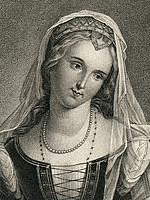
\includegraphics[width=0.3\textwidth]{img/laura.jpg}
    \caption{The figure accompanying question~\protect\ref{itm:platoniclove}}
    \label{fig:laura}
\end{figure}

\begin{figure}
    \centering
    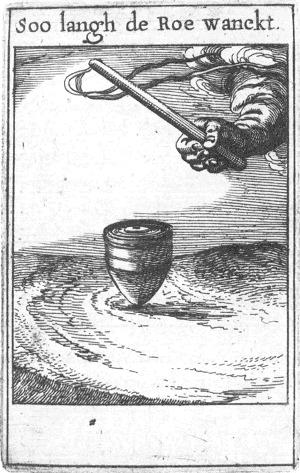
\includegraphics[width=0.3\textwidth]{img/emblem.jpg}
    \caption{The figure accompanying question~\protect\ref{itm:emblem}. This figure was accompanied by the following text: ``Soo lang de Roe wanckt. Veel mensche zijn deughdelijck, soo langh zy onder het kruys en verdruckinghe leven: maer als de Roede van den eers is, soo worden zy luy in den dienste Goods. Ghelijuck enen Drijf-tol, die niet meer gheslaghen of ghegispt en wort, die valt haest in onmacht ende blijft ligghen. Uit: Roemer Visscher, Sinnepoppen.'' In the original test a modern Dutch translation was also provided.}
    \label{fig:emblem}
\end{figure}

%    \chapter{Concept map}

\label{ch:concept_map}

\lstinputlisting{../software/database/concept_map.json}

%    \chapter{Flashcards}

\label{ch:flashcards}

\lstinputlisting{../software/database/flashcards.json}

%    \chapter{Questions measuring comprehension levels}

\label{ch:test}

\lstinputlisting{../software/database/itembank.json}

    \clearpage
    \section{Use case diagram for logging in and storing user information}
\label{app:loginusecase}
\begin{figure}[h!]
\centering
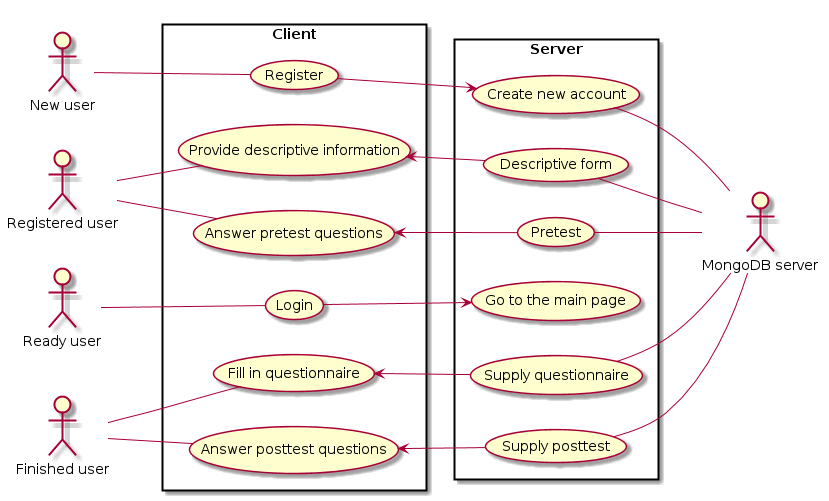
\includegraphics[width=\textwidth]{img/loginusecase.png}
\end{figure}

    \clearpage
    \section{Use case diagram for main purposes}
\label{app:mainusecase}
\begin{figure}[h!]
\centering
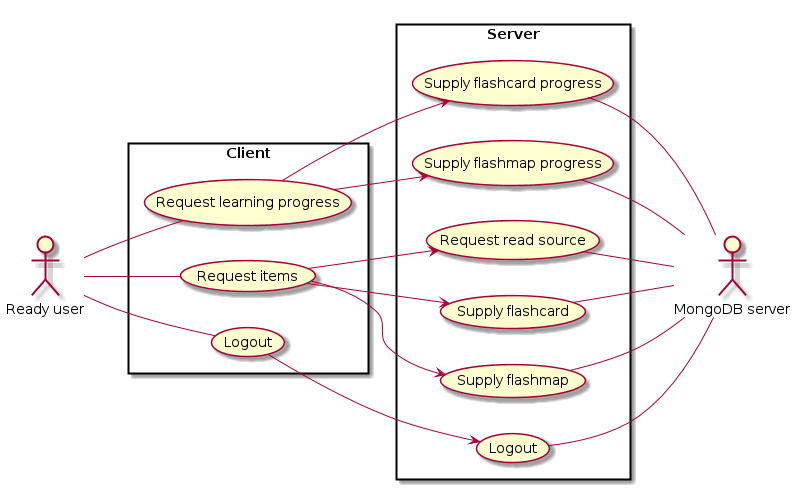
\includegraphics[width=\textwidth]{img/mainusecase.png}
\end{figure}

    \clearpage
%    \section{Class diagram for the datamodel}
\label{app:classdiagram}
\begin{figure}[h!]
\centering
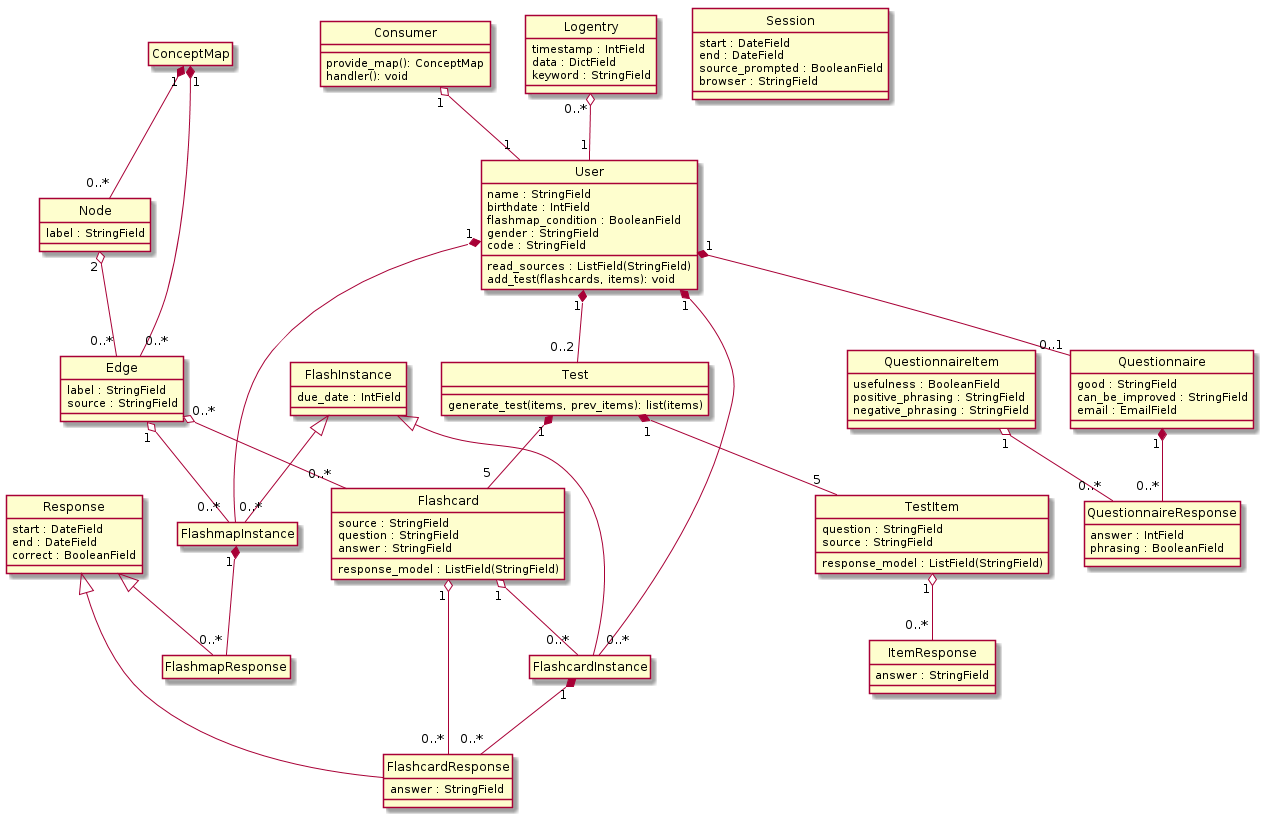
\includegraphics[height=\textheight-10ex]{img/classdiagram.png}
\end{figure}

%    \clearpage
    \section{Activity diagram for logging in}
\label{app:loginactivity}
\begin{figure}[h!]
\centering
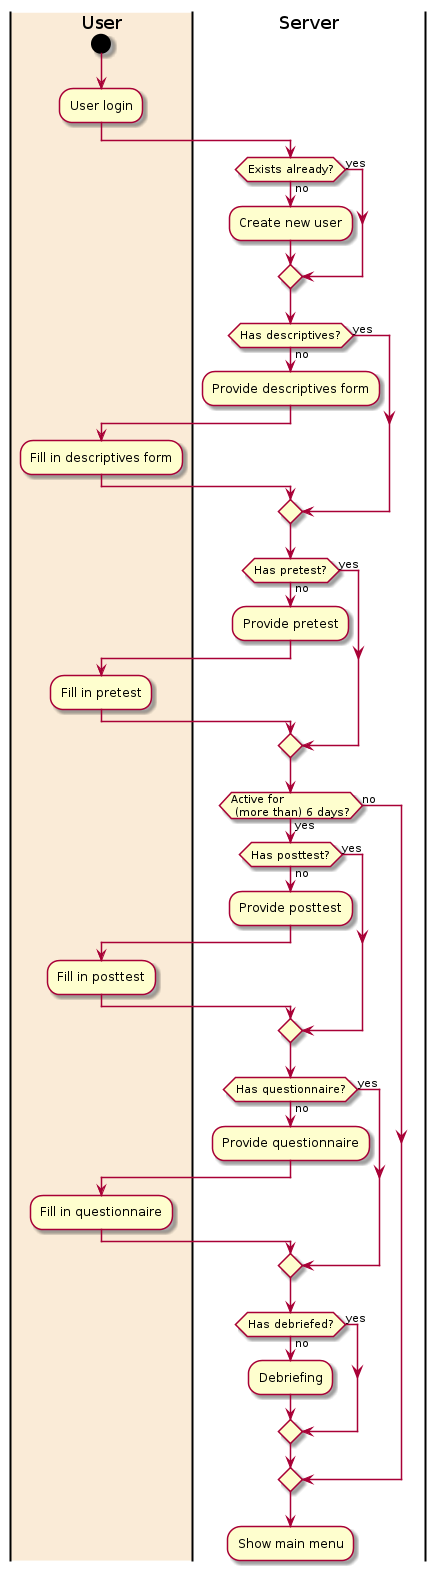
\includegraphics[height=\textheight-10ex]{img/loginactivity.png}
\end{figure}

    \clearpage
    \section{Activity diagram learning functionality}
\label{app:learningactivity}
\begin{figure}[h!]
\centering
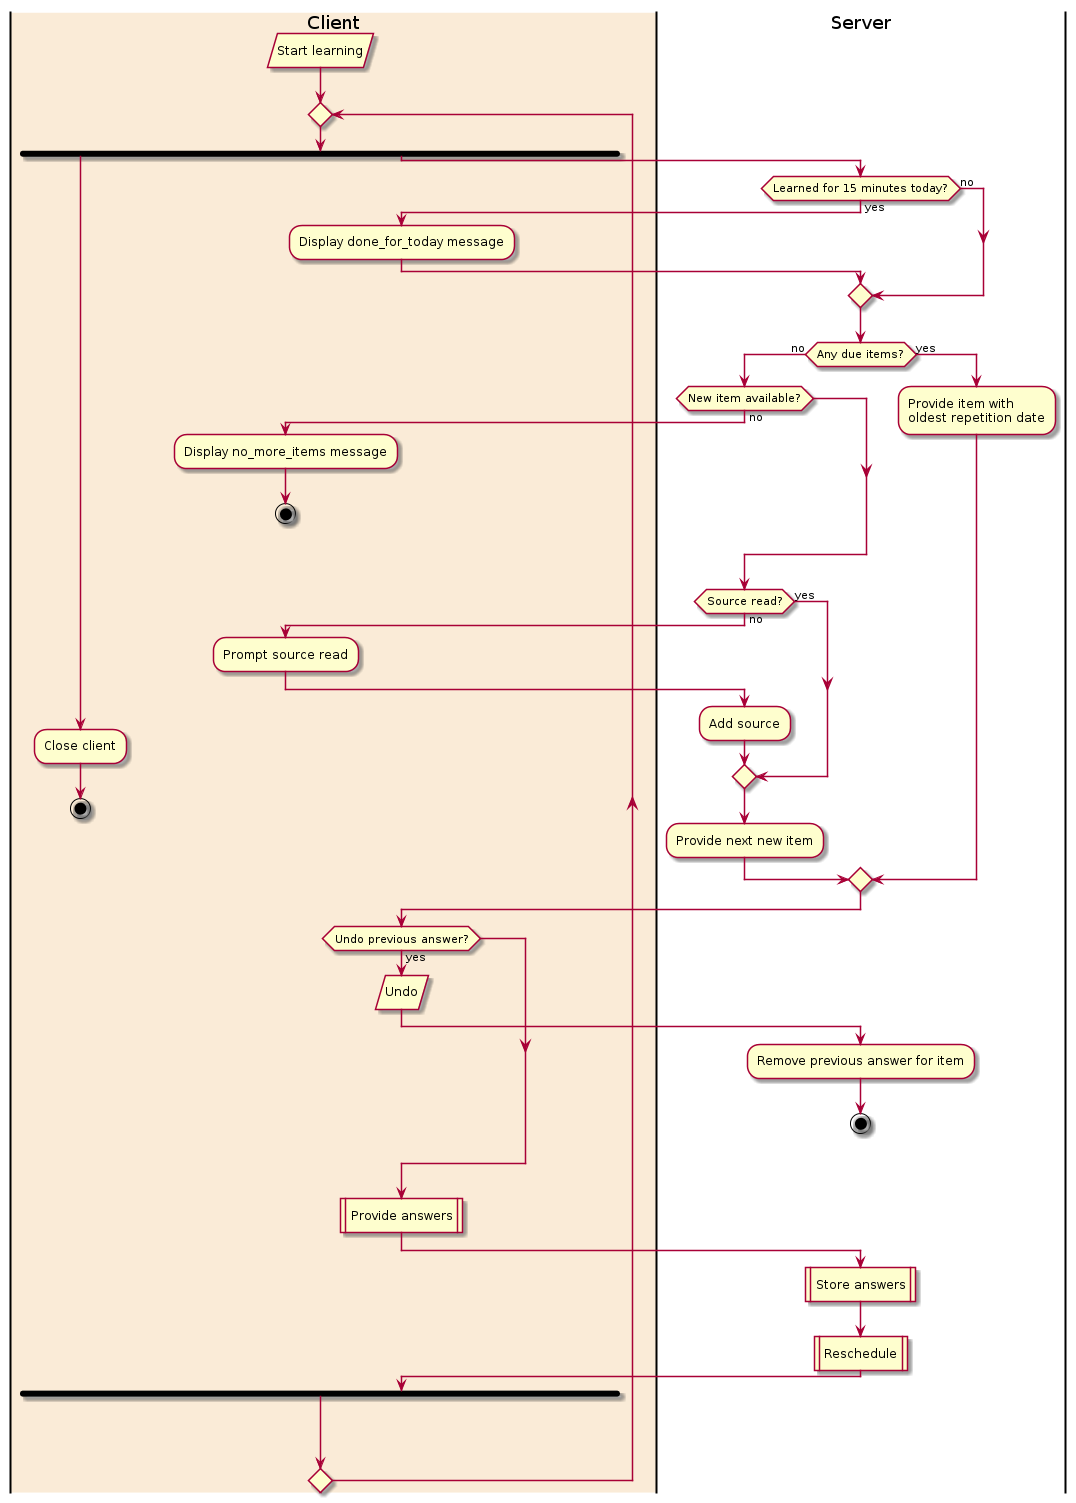
\includegraphics[width=.9\textwidth]{img/learningactivitygen.png}
\caption{General schema}
\end{figure}
\begin{figure}[h!]
\centering
\includegraphics[width=\textwidth]{img/learningserver.png}
\caption{Instance scheduling on the server}
\end{figure}
\begin{figure}[h!]
\centering
\includegraphics[width=\textwidth]{img/learningclient.png}
\caption{Prompting an instance on the client}
\end{figure}

    \clearpage
    \includepdf[pages={1-}]{../software/server/doc/build/latex/Flashmapserver.pdf}
\end{appendices}
    \chapter{Pretest and posttest statistics}
\label{app:learning_gain}

\section{Descriptives of the knowledge questions}

\begin{longtable}[c]{@{}lrrrrrrrrrr@{}}
\caption{Flashcard condition}\\
\endfirsthead
\endhead
\toprule\addlinespace
& N & min & max & mean & var & skew & kurt & norm-t &
norm-p & $\alpha$
\\
\addlinespace
\midrule
\textbf{ctt:total} & 24 & 0 & 6 & 1.29 & 4.13 & 1.34 & 0.40 & 8.732 &
0.0127 & 0.6958
\\\addlinespace
\textbf{ctt:pretest} & 12 & 0 & 3 & 0.67 & 1.15 & 1.16 & -0.19 & 4.546 &
0.1030 & 0.4290
\\\addlinespace
\textbf{ctt:posttest} & 12 & 0 & 6 & 1.92 & 6.63 & 0.70 & -1.29 & 3.371
& 0.1854 & 0.7261
\\\addlinespace
\textbf{ctt:abs\_learn\_gain} & 12 & -3 & 6 & 1.25 & 8.39 & 0.47 & -0.84
& 0.900 & 0.6378 & 0.4290
\\\addlinespace
\textbf{ctt:rel\_learn\_gain} & 12 & 0 & 0 & 0.04 & 0.00 & 0.43 & -0.86
& 0.810 & 0.6671 & 0.4290
\\\addlinespace
\textbf{irt:total} & 24 & -1 & 4 & -0.03 & 3.05 & 1.05 & 0.04 & 5.537 &
0.0627 & 0.4556
\\\addlinespace
\textbf{irt:pretest} & 12 & 0 & 0 & 0.00 & 0.08 & 0.62 & 0.07 & 2.059 &
0.3573 & 0.0687
\\\addlinespace
\textbf{irt:posttest} & 12 & -2 & 3 & -0.01 & 2.70 & 0.61 & 0.63 & 3.146
& 0.2074 & 0.3769
\\\addlinespace
\textbf{irt:abs\_learn\_gain} & 12 & -2 & 3 & -0.01 & 2.87 & 0.91 & 0.61
& 4.553 & 0.1026 & 0.0687
\\\addlinespace
\textbf{irt:rel\_learn\_gain} & 12 & 0 & 0 & 0.02 & 0.00 & 0.90 & 0.59 &
4.487 & 0.1061 & 0.0687
\\\addlinespace
\textbf{fixed irt:total} & 24 & -4 & 3 & -0.83 & 4.14 & 0.58 & -0.36
& 1.812 & 0.4042 & 0.5294
\\\addlinespace
\textbf{fixed irt:pretest} & 12 & 1 & 3 & 2.60 & 0.17 & 0.43 & 0.39 &
2.010 & 0.3661 & 0.1088
\\\addlinespace
\textbf{fixed irt:posttest} & 12 & -2 & 3 & -0.07 & 2.71 & 0.61 &
0.63 & 3.188 & 0.2031 & 0.3774
\\\addlinespace
\textbf{fixed irt:abs\_learn\_gain} & 12 & -4 & 1 & -2.67 & 2.91 &
1.01 & 0.64 & 5.199 & 0.0743 & 0.1088
\\\addlinespace
\textbf{fixed irt:rel\_learn\_gain} & 12 & 0 & 0 & -0.03 & 0.00 &
1.01 & 0.62 & 5.132 & 0.0769 & 0.1088
\\\addlinespace
\bottomrule
    \label{tab:know_fc}
\end{longtable}

\begin{figure}
    \centering
    \includegraphics[width=.7\textwidth]{img/know_fc_diff.png}
    \caption{A histogram depicting the scores on the knowledge section of the pre- and posttest per item by flashcard users}
    \label{fig:know_fc_diff}
\end{figure}
\begin{figure}
    \centering
    \includegraphics[width=.7\textwidth]{img/know_fc_abil.png}
    \caption{A histogram depicting the scores on the knowledge section of the pre- and posttest per flashcard user}
    \label{fig:know_fc_abil}
\end{figure}

\begin{longtable}[c]{@{}lrrrrrrrrrr@{}}
\caption{Flashmap condition}
\endfirsthead
\endhead
\toprule\addlinespace
& N & min & max & mean & var & skew & kurt & norm-t &
norm-p & $\alpha$
\\\addlinespace
\midrule
\textbf{ctt:total} & 22 & 0 & 7 & 1.32 & 4.89 & 1.48 & 0.77 & 10.348 &
0.0057 & 0.7424
\\\addlinespace
\textbf{ctt:pretest} & 11 & 0 & 1 & 0.18 & 0.16 & 1.65 & 0.72 & 9.711 &
0.0078 & -0.1132
\\\addlinespace
\textbf{ctt:posttest} & 11 & 0 & 7 & 2.45 & 7.27 & 0.45 & -1.31 & 2.304
& 0.3160 & 0.6841
\\\addlinespace
\textbf{ctt:abs\_learn\_gain} & 11 & -1 & 7 & 2.27 & 7.42 & 0.45 & -1.14
& 1.448 & 0.4848 & -0.1132
\\\addlinespace
\textbf{ctt:rel\_learn\_gain} & 11 & 0 & 0 & 0.05 & 0.00 & 0.44 & -1.15
& 1.490 & 0.4747 & -0.1132
\\\addlinespace
\textbf{irt:total} & 22 & -2 & 4 & -0.03 & 3.02 & 0.62 & 0.46 & 3.124 &
0.2097 & 0.3942
\\\addlinespace
\textbf{irt:pretest} & 11 & 0 & 0 & -0.00 & 0.00 & 1.65 & 0.72 & 9.711 &
0.0078 & 0.0000
\\\addlinespace
\textbf{irt:posttest} & 11 & -1 & 1 & -0.00 & 0.76 & -0.00 & 2.50 &
6.534 & 0.0381 & 0.1362
\\\addlinespace
\textbf{irt:abs\_learn\_gain} & 11 & -1 & 1 & -0.00 & 0.76 & -0.00 &
2.50 & 6.534 & 0.0381 & 0.0000
\\\addlinespace
\textbf{irt:rel\_learn\_gain} & 11 & 0 & 0 & 0.02 & 0.00 & 0.00 & 2.50 &
7.592 & 0.0225 & 0.0000
\\\addlinespace
\textbf{fixed irt:total} & 22 & -4 & 3 & -0.80 & 3.94 & 0.17 & 0.04 &
0.556 & 0.7575 & 0.4530
\\\addlinespace
\textbf{fixed irt:pretest} & 11 & 0 & 0 & 0.11 & 0.00 & 0.00 & -3.00
& 1.057 & 0.5894 & 0.0000
\\\addlinespace
\textbf{fixed irt:posttest} & 11 & 2 & 4 & 3.27 & 0.15 & -0.02 & 2.44
& 6.403 & 0.0407 & 0.1020
\\\addlinespace
\textbf{fixed irt:abs\_learn\_gain} & 11 & 2 & 4 & 3.17 & 0.15 &
-0.02 & 2.44 & 6.403 & 0.0407 & 0.0000
\\\addlinespace
\textbf{fixed irt:rel\_learn\_gain} & 11 & 0 & 0 & 0.07 & 0.00 &
-0.02 & 2.44 & 6.403 & 0.0407 & 0.0000
\\\addlinespace
\bottomrule
    \label{tab:know_fm}
\end{longtable}

\begin{figure}
    \centering
    \includegraphics[width=.7\textwidth]{img/know_fm_diff.png}
    \caption{A histogram depicting the scores on the knowledge section of the pre- and posttest per item by flashmap users}
    \label{fig:know_fm_diff}
\end{figure}
\begin{figure}
    \centering
    \includegraphics[width=.7\textwidth]{img/know_fm_abil.png}
    \caption{A histogram depicting the scores on the knowledge section of the pre- and posttest per flashmap user}
    \label{fig:know_fm_abil}
\end{figure}

\begin{longtable}[c]{@{}lrrrrrrrrrr@{}}
\caption{Combined conditions}
\endfirsthead
\endhead
\toprule\addlinespace
& N & min & max & mean & var & skew & kurt & norm-t &
norm-p & $\alpha$
\\\addlinespace
\midrule
\textbf{ctt:total} & 46 & 0 & 7 & 1.30 & 4.39 & 1.42 & 0.64 & 14.471 &
0.0007 & 0.7112
\\\addlinespace
\textbf{ctt:pretest} & 23 & 0 & 3 & 0.43 & 0.71 & 1.83 & 2.28 & 17.317 &
0.0002 & 0.3937
\\\addlinespace
\textbf{ctt:posttest} & 23 & 0 & 7 & 2.17 & 6.70 & 0.58 & -1.30 & 6.839
& 0.0327 & 0.6851
\\\addlinespace
\textbf{ctt:abs\_learn\_gain} & 23 & -3 & 7 & 1.74 & 7.84 & 0.40 & -0.93
& 2.023 & 0.3637 & 0.3937
\\\addlinespace
\textbf{ctt:rel\_learn\_gain} & 23 & 0 & 0 & 0.03 & 0.00 & 0.39 & -0.93
& 1.977 & 0.3722 & 0.3937
\\\addlinespace
\textbf{irt:total} & 46 & -3 & 5 & -0.10 & 4.92 & 0.98 & -0.23 & 7.303 &
0.0259 & 0.5856
\\\addlinespace
\textbf{irt:pretest} & 23 & -2 & 2 & -0.00 & 1.22 & 0.97 & 2.19 & 9.614
& 0.0082 & 0.2141
\\\addlinespace
\textbf{irt:posttest} & 23 & -3 & 3 & -0.02 & 3.68 & 0.87 & -0.19 &
3.757 & 0.1528 & 0.4740
\\\addlinespace
\textbf{irt:abs\_learn\_gain} & 23 & -4 & 4 & -0.02 & 5.31 & 0.42 &
-0.29 & 0.967 & 0.6166 & 0.2141
\\\addlinespace
\textbf{irt:rel\_learn\_gain} & 23 & 0 & 0 & 0.01 & 0.00 & 0.38 & -0.27
& 0.833 & 0.6592 & 0.2141
\\\addlinespace
\textbf{fixed irt:total} & 46 & -5 & 3 & -1.85 & 5.68 & 0.80 & -0.29
& 5.224 & 0.0734 & 0.6710
\\\addlinespace
\textbf{fixed irt:pretest} & 23 & -2 & 2 & -0.01 & 1.22 & 0.98 & 2.19
& 9.677 & 0.0079 & 0.2142
\\\addlinespace
\textbf{fixed irt:posttest} & 23 & -4 & 3 & -0.88 & 5.74 & 0.31 &
-0.53 & 0.564 & 0.7541 & 0.5859
\\\addlinespace
\textbf{fixed irt:abs\_learn\_gain} & 23 & -7 & 4 & -0.88 & 8.23 &
-0.21 & 0.11 & 0.742 & 0.6900 & 0.2142
\\\addlinespace
\textbf{fixed irt:rel\_learn\_gain} & 23 & 0 & 0 & 0.00 & 0.00 &
-0.26 & 0.19 & 1.015 & 0.6019 & 0.2142
\\\addlinespace
\bottomrule
    \label{tab:know_gen}
\end{longtable}

\begin{figure}
    \centering
    \includegraphics[width=.7\textwidth]{img/know_gen_diff.png}
    \caption{A histogram depicting the scores on the knowledge section of the pre- and posttest per item}
    \label{fig:know_gen_diff}
\end{figure}
\begin{figure}
    \centering
    \includegraphics[width=.7\textwidth]{img/know_gen_abil.png}
    \caption{A histogram depicting the scores on the knowledge section of the pre- and posttest per user}
    \label{fig:know_gen_abil}
\end{figure}

\FloatBarrier
\section{Comparisons of the knowledge questions}

\FloatBarrier
\subsection{Pre- and posttest comparisons}

\begin{longtable}[c]{@{}lrrrr@{}}
\caption{Flashcard condition}
\endfirsthead
\endhead
\toprule\addlinespace
& \textbf{MW k} & \textbf{MW p} &
\textbf{t-test k} & \textbf{t-test p}
\\\addlinespace
\midrule
\textbf{ctt} & -1.552 & 0.1348 & -1.552 & 0.1418
\\\addlinespace
\textbf{irt} & 0.016 & 0.9872 & 0.016 & 0.9873
\\\addlinespace
\textbf{fixed irt} & 5.454 & 0.0000 & 5.454 & 0.0001
\\\addlinespace
\bottomrule
    \label{tab:know_pp_fc_comp}
\end{longtable}

\begin{longtable}[c]{@{}lrrrr@{}}
\caption{Flashmap condition}
\endfirsthead
\endhead
\toprule\addlinespace
& \textbf{MW k} & \textbf{MW p} &
\textbf{t-test k} & \textbf{t-test p}
\\\addlinespace
\midrule
\textbf{ctt} & -2.764 & 0.0120 & -2.764 & 0.0192
\\\addlinespace
\textbf{irt} & -0.000 & 1.0000 & -0.000 & 1.0000
\\\addlinespace
\textbf{fixed irt} & -27.206 & 0.0000 & -27.206 & 0.0000
\\\addlinespace
\bottomrule
    \label{tab:know_pp_fm_comp}
\end{longtable}

\begin{longtable}[c]{@{}lrrrr@{}}
\caption{Combined conditions}
\endfirsthead
\endhead
\toprule\addlinespace
& \textbf{MW k} & \textbf{MW p} &
\textbf{t-test k} & \textbf{t-test p}
\\\addlinespace
\midrule
\textbf{ctt} & -3.065 & 0.0037 & -3.065 & 0.0049
\\\addlinespace
\textbf{irt} & 0.051 & 0.9597 & 0.051 & 0.9598
\\\addlinespace
\textbf{fixed irt} & 1.591 & 0.1187 & 1.591 & 0.1217
\\\addlinespace
\bottomrule
    \label{tab:know_pp_gen_comp}
\end{longtable}

\FloatBarrier
\subsection{Learning gain comparisons between conditions}

\begin{longtable}[c]{@{}lrrrr@{}}
\caption{Classical test theory}
\endfirsthead
\endhead
\toprule\addlinespace
& \textbf{MW k} & \textbf{MW p} &
\textbf{t-test k} & \textbf{t-test p}
\\\addlinespace
\midrule
\textbf{total} & -0.042 & 0.9664 & -0.042 & 0.9665
\\\addlinespace
\textbf{pretest} & 1.407 & 0.1739 & 1.456 & 0.1669
\\\addlinespace
\textbf{posttest} & -0.489 & 0.6297 & -0.488 & 0.6305
\\\addlinespace
\textbf{abs\_learn\_gain} & -0.870 & 0.3940 & -0.873 & 0.3927
\\\addlinespace
\textbf{rel\_learn\_gain} & -0.747 & 0.4635 & -0.751 & 0.4611
\\\addlinespace
\bottomrule
    \label{tab:know_cond_ctt_comp}
\end{longtable}

\begin{longtable}[c]{@{}lrrrr@{}}
\caption{Item response theory}
\endfirsthead
\endhead
\toprule\addlinespace
& \textbf{MW k} & \textbf{MW p} &
\textbf{t-test k} & \textbf{t-test p}
\\\addlinespace
\midrule
\textbf{total} & -0.001 & 0.9989 & -0.001 & 0.9989
\\\addlinespace
\textbf{pretest} & 0.000 & 1.0000 & 0.000 & 1.0000
\\\addlinespace
\textbf{posttest} & -0.014 & 0.9889 & -0.014 & 0.9887
\\\addlinespace
\textbf{abs\_learn\_gain} & -0.014 & 0.9892 & -0.014 & 0.9889
\\\addlinespace
\textbf{rel\_learn\_gain} & 0.072 & 0.9436 & 0.074 & 0.9423
\\\addlinespace
\bottomrule
    \label{tab:know_cond_irt_comp}
\end{longtable}

\begin{longtable}[c]{@{}lrrrr@{}}
\caption{Item response theory with fixed item difficulties}
\endfirsthead
\endhead
\toprule\addlinespace
& \textbf{MW k} & \textbf{MW p} &
\textbf{t-test k} & \textbf{t-test p}
\\\addlinespace
\midrule
\textbf{total} & -0.050 & 0.9602 & -0.050 & 0.9602
\\\addlinespace
\textbf{pretest} & 20.261 & 0.0000 & 21.204 & 0.0000
\\\addlinespace
\textbf{posttest} & -6.549 & 0.0000 & -6.821 & 0.0000
\\\addlinespace
\textbf{abs\_learn\_gain} & -11.067 & 0.0000 & -11.531 & 0.0000
\\\addlinespace
\textbf{rel\_learn\_gain} & -10.401 & 0.0000 & -10.845 & 0.0000
\\\addlinespace
\bottomrule
    \label{tab:know_cond_adj_irt_comp}
\end{longtable}

\begin{figure}
    \centering
    \includegraphics[width=.7\textwidth]{img/know_gain_diff.png}
    \caption{A comparison of figure~\protect\ref{fig:know_fc_diff} and~\protect\ref{fig:know_fm_diff}, with the pretest score subtracted from the posttest score}
    \label{fig:know_gain_diff}
\end{figure}

\FloatBarrier
\section{Descriptives of the comprehension questions}

\begin{longtable}[c]{@{}lrrrrrrrrrr@{}}
\caption{Flashcard condition}
\endfirsthead
\endhead
\toprule\addlinespace
& N & min & max & mean & var & skew & kurt & norm-t &
norm-p & $\alpha$
\\\addlinespace
\midrule
\textbf{ctt:total} & 24 & 0 & 6 & 1.33 & 4.23 & 1.19 & -0.05 & 6.646 &
0.0361 & 0.7215
\\\addlinespace
\textbf{ctt:pretest} & 12 & 0 & 4 & 0.33 & 1.33 & 3.02 & 7.09 & 33.648 &
0.0000 & 0.7670
\\\addlinespace
\textbf{ctt:posttest} & 12 & 0 & 6 & 2.33 & 5.33 & 0.41 & -1.25 & 2.077
& 0.3540 & 0.6450
\\\addlinespace
\textbf{ctt:abs\_learn\_gain} & 12 & 0 & 6 & 2.00 & 5.45 & 0.72 & -0.96
& 2.091 & 0.3516 & 0.6450
\\\addlinespace
\textbf{ctt:rel\_learn\_gain} & 12 & 0 & 0 & 0.07 & 0.00 & 0.72 & -0.95
& 2.097 & 0.3504 & 0.6450
\\\addlinespace
\textbf{irt:total} & 24 & -2 & 4 & 0.05 & 4.71 & 0.80 & -0.83 & 4.030 &
0.1333 & 0.6583
\\\addlinespace
\textbf{irt:pretest} & 12 & -1 & 4 & -0.09 & 2.62 & 2.47 & 5.19 & 26.077
& 0.0000 & 0.3406
\\\addlinespace
\textbf{irt:posttest} & 12 & -2 & 2 & 0.01 & 3.51 & 0.00 & -1.31 & 1.869
& 0.3929 & 0.7510
\\\addlinespace
\textbf{irt:abs\_learn\_gain} & 12 & -3 & 3 & 0.10 & 5.54 & -0.07 &
-1.19 & 1.211 & 0.5459 & 0.3406
\\\addlinespace
\textbf{irt:rel\_learn\_gain} & 12 & 0 & 0 & 0.02 & 0.00 & -0.15 & -1.11
& 0.886 & 0.6420 & 0.3406
\\\addlinespace
\textbf{fixed irt:total} & 24 & -3 & 3 & -1.15 & 3.83 & 0.90 & -0.52
& 4.058 & 0.1315 & 0.6673
\\\addlinespace
\textbf{fixed irt:pretest} & 12 & 0 & 5 & 0.42 & 2.58 & 2.72 & 6.04 &
29.551 & 0.0000 & 0.3207
\\\addlinespace
\textbf{fixed irt:posttest} & 12 & -3 & 1 & -0.87 & 3.16 & 0.03 &
-1.30 & 1.835 & 0.3994 & 0.7480
\\\addlinespace
\textbf{fixed irt:abs\_learn\_gain} & 12 & -5 & 2 & -1.28 & 5.01 &
-0.15 & -1.04 & 0.652 & 0.7218 & 0.3207
\\\addlinespace
\textbf{fixed irt:rel\_learn\_gain} & 12 & 0 & 0 & -0.01 & 0.00 &
-0.29 & -0.81 & 0.411 & 0.8142 & 0.3207
\\\addlinespace
\bottomrule
    \label{tab:comp_fc}
\end{longtable}

\begin{figure}
    \centering
    \includegraphics[width=.7\textwidth]{img/comp_fc_diff.png}
    \caption{A histogram depicting the scores on the comprehension section of the pre- and posttest per item by flashcard users}
    \label{fig:comp_fc_diff}
\end{figure}
\begin{figure}
    \centering
    \includegraphics[width=.7\textwidth]{img/comp_fc_abil.png}
    \caption{A histogram depicting the scores on the comprehension section of the pre- and posttest per flashcard user}
    \label{fig:comp_fc_abil}
\end{figure}

\begin{longtable}[c]{@{}lrrrrrrrrrr@{}}
\caption{Flashmap condition}
\endfirsthead
\endhead
\toprule\addlinespace
& N & min & max & mean & var & skew & kurt & norm-t &
norm-p & $\alpha$
\\\addlinespace
\midrule
\textbf{ctt:total} & 22 & 0 & 8 & 1.27 & 3.92 & 2.06 & 4.13 & 22.828 &
0.0000 & 0.7202
\\\addlinespace
\textbf{ctt:pretest} & 11 & 0 & 4 & 0.82 & 1.56 & 1.64 & 1.82 & 12.332 &
0.0021 & 0.5351
\\\addlinespace
\textbf{ctt:posttest} & 11 & 0 & 8 & 1.73 & 6.22 & 1.58 & 1.62 & 11.397
& 0.0034 & 0.7566
\\\addlinespace
\textbf{ctt:abs\_learn\_gain} & 11 & -1 & 4 & 0.91 & 2.89 & 1.04 & -0.35
& 3.526 & 0.1715 & 0.5351
\\\addlinespace
\textbf{ctt:rel\_learn\_gain} & 11 & 0 & 0 & 0.04 & 0.00 & 1.09 & -0.23
& 3.961 & 0.1380 & 0.5351
\\\addlinespace
\textbf{irt:total} & 22 & -1 & 3 & 0.01 & 2.83 & 0.65 & -1.02 & 3.743 &
0.1539 & 0.6260
\\\addlinespace
\textbf{irt:pretest} & 11 & -1 & 3 & -0.00 & 2.98 & 0.91 & -0.34 & 2.786
& 0.2483 & 0.5317
\\\addlinespace
\textbf{irt:posttest} & 11 & -2 & 2 & 0.01 & 3.41 & 0.19 & -1.62 & 4.801
& 0.0907 & 0.6901
\\\addlinespace
\textbf{irt:abs\_learn\_gain} & 11 & -1 & 2 & 0.01 & 1.71 & 1.00 & -0.12
& 3.564 & 0.1683 & 0.5317
\\\addlinespace
\textbf{irt:rel\_learn\_gain} & 11 & 0 & 0 & 0.02 & 0.00 & 0.99 & -0.11
& 3.521 & 0.1720 & 0.5317
\\\addlinespace
\textbf{fixed irt:total} & 22 & -1 & 3 & 0.05 & 2.92 & 0.66 & -1.01 &
3.727 & 0.1551 & 0.6277
\\\addlinespace
\textbf{fixed irt:pretest} & 11 & 0 & 4 & 1.54 & 2.10 & 0.93 & -0.32
& 2.893 & 0.2354 & 0.4888
\\\addlinespace
\textbf{fixed irt:posttest} & 11 & -1 & 3 & 0.57 & 3.81 & 0.15 &
-1.64 & 5.133 & 0.0768 & 0.6957
\\\addlinespace
\textbf{fixed irt:abs\_learn\_gain} & 11 & -2 & 1 & -0.97 & 1.88 &
1.08 & 0.01 & 4.284 & 0.1174 & 0.4888
\\\addlinespace
\textbf{fixed irt:rel\_learn\_gain} & 11 & 0 & 0 & 0.00 & 0.00 & 1.08
& 0.01 & 4.277 & 0.1178 & 0.4888
\\\addlinespace
\bottomrule
    \label{tab:comp_fm}
\end{longtable}

\begin{figure}
    \centering
    \includegraphics[width=.7\textwidth]{img/comp_fm_diff.png}
    \caption{A histogram depicting the scores on the comprehension section of the pre- and posttest per item by flashmap users}
    \label{fig:comp_fm_diff}
\end{figure}
\begin{figure}
    \centering
    \includegraphics[width=.7\textwidth]{img/comp_fm_abil.png}
    \caption{A histogram depicting the scores on the comprehension section of the pre- and posttest per flashmap user}
    \label{fig:comp_fm_abil}
\end{figure}

\begin{longtable}[c]{@{}lrrrrrrrrrr@{}}
\caption{Combined conditions}
\endfirsthead
\endhead
\toprule\addlinespace
& N & min & max & mean & var & skew & kurt & norm-t &
norm-p & $\alpha$
\\\addlinespace
\midrule
\textbf{ctt:total} & 46 & 0 & 8 & 1.30 & 3.99 & 1.58 & 1.77 & 19.890 &
0.0000 & 0.7140
\\\addlinespace
\textbf{ctt:pretest} & 23 & 0 & 4 & 0.57 & 1.44 & 2.19 & 3.53 & 23.159 &
0.0000 & 0.6350
\\\addlinespace
\textbf{ctt:posttest} & 23 & 0 & 8 & 2.04 & 5.59 & 0.98 & -0.02 & 4.808
& 0.0903 & 0.6951
\\\addlinespace
\textbf{ctt:abs\_learn\_gain} & 23 & -1 & 6 & 1.48 & 4.35 & 0.97 & -0.34
& 4.419 & 0.1097 & 0.6350
\\\addlinespace
\textbf{ctt:rel\_learn\_gain} & 23 & 0 & 0 & 0.05 & 0.00 & 0.95 & -0.42
& 4.277 & 0.1178 & 0.6350
\\\addlinespace
\textbf{irt:total} & 46 & -1 & 3 & 0.00 & 2.33 & 0.81 & -0.90 & 8.324 &
0.0156 & 0.6015
\\\addlinespace
\textbf{irt:pretest} & 23 & -1 & 4 & 0.01 & 2.56 & 1.65 & 1.53 & 13.943
& 0.0009 & 0.4629
\\\addlinespace
\textbf{irt:posttest} & 23 & -1 & 2 & 0.00 & 2.04 & 0.19 & -1.52 &
11.285 & 0.0035 & 0.6781
\\\addlinespace
\textbf{irt:abs\_learn\_gain} & 23 & -3 & 3 & -0.01 & 2.86 & 0.32 &
-0.85 & 1.311 & 0.5192 & 0.4629
\\\addlinespace
\textbf{irt:rel\_learn\_gain} & 23 & 0 & 0 & 0.02 & 0.00 & 0.24 & -0.77
& 0.786 & 0.6749 & 0.4629
\\\addlinespace
\textbf{fixed irt:total} & 46 & -2 & 2 & -0.62 & 2.30 & 0.82 & -0.86
& 8.005 & 0.0183 & 0.6058
\\\addlinespace
\textbf{fixed irt:pretest} & 23 & -1 & 4 & 0.04 & 2.52 & 1.66 & 1.54
& 13.979 & 0.0009 & 0.4618
\\\addlinespace
\textbf{fixed irt:posttest} & 23 & -1 & 2 & -0.23 & 1.97 & 0.17 &
-1.56 & 12.676 & 0.0018 & 0.6732
\\\addlinespace
\textbf{fixed irt:abs\_learn\_gain} & 23 & -3 & 2 & -0.26 & 2.85 &
0.27 & -0.87 & 1.246 & 0.5362 & 0.4618
\\\addlinespace
\textbf{fixed irt:rel\_learn\_gain} & 23 & 0 & 0 & 0.02 & 0.00 & 0.18
& -0.76 & 0.640 & 0.7262 & 0.4618
\\\addlinespace
\bottomrule
    \label{tab:comp_gen}
\end{longtable}

\begin{figure}
    \centering
    \includegraphics[width=.7\textwidth]{img/comp_gen_diff.png}
    \caption{A histogram depicting the scores on the comprehension section of the pre- and posttest per item by users}
    \label{fig:comp_gen_diff}
\end{figure}
\begin{figure}
    \centering
    \includegraphics[width=.7\textwidth]{img/comp_gen_abil.png}
    \caption{A histogram depicting the scores on the comprehension section of the pre- and posttest per user}
    \label{fig:comp_gen_abil}
\end{figure}

\section{Comparisons of the comprehension questions}

\subsection{Pre- and posttest comparisons}

\begin{longtable}[c]{@{}lrrrr@{}}
\caption{Flashcard condition}
\endfirsthead
\endhead
\toprule\addlinespace
& \textbf{MW k} & \textbf{MW p} &
\textbf{t-test k} & \textbf{t-test p}
\\\addlinespace
\midrule
\textbf{ctt} & -2.683 & 0.0136 & -2.683 & 0.0162
\\\addlinespace
\textbf{irt} & -0.146 & 0.8852 & -0.146 & 0.8852
\\\addlinespace
\textbf{fixed irt} & 1.856 & 0.0768 & 1.856 & 0.0770
\\\addlinespace
\bottomrule
    \label{tab:comp_pp_fc_comp}
\end{longtable}

\begin{longtable}[c]{@{}lrrrr@{}}
\caption{Flashmap condition}
\endfirsthead
\endhead
\toprule\addlinespace
& \textbf{MW k} & \textbf{MW p} &
\textbf{t-test k} & \textbf{t-test p}
\\\addlinespace
\midrule
\textbf{ctt} & -1.081 & 0.2926 & -1.081 & 0.2971
\\\addlinespace
\textbf{irt} & -0.018 & 0.9854 & -0.018 & 0.9854
\\\addlinespace
\textbf{fixed irt} & 1.318 & 0.2024 & 1.318 & 0.2036
\\\addlinespace
\bottomrule
    \label{tab:comp_pp_fm_comp}
\end{longtable}

\begin{longtable}[c]{@{}lrrrr@{}}
\caption{Combined conditions}
\endfirsthead
\endhead
\toprule\addlinespace
& \textbf{MW k} & \textbf{MW p} &
\textbf{t-test k} & \textbf{t-test p}
\\\addlinespace
\midrule
\textbf{ctt} & -2.674 & 0.0105 & -2.674 & 0.0116
\\\addlinespace
\textbf{irt} & 0.023 & 0.9818 & 0.023 & 0.9818
\\\addlinespace
\textbf{fixed irt} & 0.595 & 0.5549 & 0.595 & 0.5549
\\\addlinespace
\bottomrule
    \label{tab:comp_pp_gen_comp}
\end{longtable}

\FloatBarrier
\subsection{Learning gain comparisons between conditions}

\begin{longtable}[c]{@{}lrrrr@{}}
\caption{Classical test theory}
\endfirsthead
\endhead
\toprule\addlinespace
& \textbf{MW k} & \textbf{MW p} &
\textbf{t-test k} & \textbf{t-test p}
\\\addlinespace
\midrule
\textbf{total} & 0.102 & 0.9195 & 0.102 & 0.9194
\\\addlinespace
\textbf{pretest} & -0.967 & 0.3446 & -0.963 & 0.3466
\\\addlinespace
\textbf{posttest} & 0.605 & 0.5515 & 0.603 & 0.5531
\\\addlinespace
\textbf{abs\_learn\_gain} & 1.270 & 0.2179 & 1.288 & 0.2124
\\\addlinespace
\textbf{rel\_learn\_gain} & 1.197 & 0.2448 & 1.211 & 0.2399
\\\addlinespace
\bottomrule
    \label{tab:comp_cond_ctt_comp}
\end{longtable}

\begin{longtable}[c]{@{}lrrrr@{}}
\caption{Item response theory}
\endfirsthead
\endhead
\toprule\addlinespace
& \textbf{MW k} & \textbf{MW p} &
\textbf{t-test k} & \textbf{t-test p}
\\\addlinespace
\midrule
\textbf{total} & 0.071 & 0.9436 & 0.072 & 0.9430
\\\addlinespace
\textbf{pretest} & -0.132 & 0.8961 & -0.132 & 0.8965
\\\addlinespace
\textbf{posttest} & -0.002 & 0.9982 & -0.002 & 0.9982
\\\addlinespace
\textbf{abs\_learn\_gain} & 0.112 & 0.9116 & 0.115 & 0.9097
\\\addlinespace
\textbf{rel\_learn\_gain} & 0.064 & 0.9496 & 0.066 & 0.9484
\\\addlinespace
\bottomrule
    \label{tab:comp_cond_irt_comp}
\end{longtable}

\begin{longtable}[c]{@{}lrrrr@{}}
\caption{Item response theory with fixed item difficulties}
\endfirsthead
\endhead
\toprule\addlinespace
& \textbf{MW k} & \textbf{MW p} &
\textbf{t-test k} & \textbf{t-test p}
\\\addlinespace
\midrule
\textbf{total} & -2.188 & 0.0340 & -2.202 & 0.0330
\\\addlinespace
\textbf{pretest} & -1.748 & 0.0950 & -1.756 & 0.0936
\\\addlinespace
\textbf{posttest} & -1.849 & 0.0785 & -1.842 & 0.0802
\\\addlinespace
\textbf{abs\_learn\_gain} & -0.407 & 0.6882 & -0.415 & 0.6826
\\\addlinespace
\textbf{rel\_learn\_gain} & -0.455 & 0.6537 & -0.465 & 0.6476
\\\addlinespace
\bottomrule
    \label{tab:comp_cond_adj_irt_comp}
\end{longtable}

\begin{figure}
    \centering
    \includegraphics[width=.7\textwidth]{img/comp_gain_diff.png}
    \caption{A comparison of figure~\protect\ref{fig:comp_fc_diff} and~\protect\ref{fig:comp_fm_diff}, with the pretest score subtracted from the posttest score}
    \label{fig:comp_gain_diff}
\end{figure}

    \chapter{Questionnaire statistics}

\section{Descriptives of Perceived Usefulness questions}

\begin{longtable}[c]{@{}lrrrrrrrrrr@{}}
\caption{Flashcard condition}
\endfirsthead
\endhead
\toprule\addlinespace
& N & min & max & mean & variance & skew & kurt & norm-t &
norm-p & $\alpha$
\\\addlinespace
\midrule
\textbf{ctt} & 12 & -4 & 14 & 6.50 & 27.36 & -0.57 & -0.52 & 1.144 &
0.5643 & 0.6432
\\\addlinespace
\textbf{irt} & 12 & -5 & 1 & -0.16 & 4.40 & -1.89 & 3.15 & 17.284 &
0.0002 & 0.6263
\\\addlinespace
\bottomrule
\end{longtable}

\includegraphics[width=\textwidth]{img/usefulness_fc_diff.png}
\includegraphics[width=\textwidth]{img/usefulness_fc_abil.png}

\begin{longtable}[c]{@{}lrrrrrrrrrr@{}}
\caption{Flashmap condition}
\endfirsthead
\toprule\addlinespace
& N & min & max & mean & variance & skew & kurt & norm-t &
norm-p & $\alpha$
\\\addlinespace
\midrule
\textbf{ctt} & 11 & 0 & 13 & 8.82 & 15.16 & -1.05 & 0.32 & 4.698 &
0.0955 & 0.6777
\\\addlinespace
\textbf{irt} & 11 & -3 & 1 & -0.15 & 1.89 & -1.41 & 1.44 & 9.670 &
0.0079 & 0.5298
\\\addlinespace
\bottomrule
\end{longtable}

\includegraphics[width=\textwidth]{img/usefulness_fm_diff.png}
\includegraphics[width=\textwidth]{img/usefulness_fm_abil.png}

\begin{longtable}[c]{@{}lrrrrrrrrrr@{}}
\caption{Combined conditions}
\endfirsthead
\toprule\addlinespace
& N & min & max & mean & variance & skew & kurt & norm-t &
norm-p & $\alpha$
\\\addlinespace
\midrule
\textbf{ctt} & 23 & -4 & 14 & 7.61 & 21.98 & -0.86 & -0.02 & 3.864 &
0.1448 & 0.6509
\\\addlinespace
\textbf{irt} & 23 & -3 & 2 & 0.49 & 1.82 & -0.73 & 0.55 & 4.058 & 0.1315
& 0.4619
\\\addlinespace
\bottomrule
\end{longtable}

\includegraphics[width=\textwidth]{img/usefulness_gen_diff.png}
\includegraphics[width=\textwidth]{img/usefulness_gen_abil.png}

\section{Descriptives of Perceived Ease of Use questions}\label{ease-of-use}

\begin{longtable}[c]{@{}lrrrrrrrrrr@{}}
\caption{Flashcard condition}
\endfirsthead
\toprule\addlinespace
& N & min & max & mean & variance & skew & kurt & norm-t &
norm-p & $\alpha$
\\\addlinespace
\midrule
\textbf{ctt} & 12 & -4 & 17 & 6.58 & 38.08 & -0.26 & -0.62 & 0.232 &
0.8904 & 0.8794
\\\addlinespace
\textbf{irt} & 12 & 0 & 4 & 0.91 & 1.87 & 1.08 & 0.52 & 5.358 & 0.0686 &
0.2295
\\\addlinespace
\bottomrule
\end{longtable}

\includegraphics[width=\textwidth]{img/easeofuse_fc_diff.png}
\includegraphics[width=\textwidth]{img/easeofuse_fc_abil.png}

\begin{longtable}[c]{@{}lrrrrrrrrrr@{}}
\caption{Flashmap condition}
\endfirsthead
\toprule\addlinespace
& N & min & max & mean & variance & skew & kurt & norm-t &
norm-p & $\alpha$
\\\addlinespace
\midrule
\textbf{ctt} & 11 & 0 & 19 & 8.27 & 26.22 & 0.50 & 0.12 & 1.725 & 0.4220
& 0.7689
\\\addlinespace
\textbf{irt} & 11 & -2 & 2 & 0.22 & 1.87 & -0.20 & 1.01 & 3.041 & 0.2186
& 0.2538
\\\addlinespace
\bottomrule
\end{longtable}

\includegraphics[width=\textwidth]{img/easeofuse_fm_diff.png}
\includegraphics[width=\textwidth]{img/easeofuse_fm_abil.png}

\begin{longtable}[c]{@{}lrrrrrrrrrr@{}}
\caption{Combined conditions}
\endfirsthead
\toprule\addlinespace
& N & min & max & mean & variance & skew & kurt & norm-t &
norm-p & $\alpha$
\\\addlinespace
\midrule
\textbf{ctt} & 23 & -4 & 19 & 7.39 & 31.70 & -0.08 & -0.10 & 0.239 &
0.8876 & 0.8285
\\\addlinespace
\bottomrule
\end{longtable}

\includegraphics[width=\textwidth]{img/easeofuse_gen_diff.png}
\includegraphics[width=\textwidth]{img/easeofuse_gen_abil.png}

\section{Comparisons of the Perceived Usefulness questions}


\begin{longtable}[c]{@{}lrrrr@{}}
\toprule\addlinespace
& \textbf{MW k} & \textbf{MW p} &
\textbf{t-test k} & \textbf{t-test p}
\\\addlinespace
\midrule
\textbf{ctt} & -1.196 & 0.2449 & -1.212 & 0.2395
\\\addlinespace
\textbf{irt} & -0.014 & 0.9891 & -0.014 & 0.9889
\\\addlinespace
\bottomrule
\end{longtable}

\includegraphics[width=\textwidth]{img/usefulness_diff.png}
\includegraphics[width=\textwidth]{img/usefulness_abil.png}

\section{Comparisons of the Perceived Usefulness questions}

\begin{longtable}[c]{@{}lrrrr@{}}
\toprule\addlinespace
& \textbf{MW k} & \textbf{MW p} &
\textbf{t-test k} & \textbf{t-test p}
\\\addlinespace
\midrule
\textbf{ctt} & -0.711 & 0.4851 & -0.717 & 0.4816
\\\addlinespace
\textbf{irt} & 1.206 & 0.2411 & 1.206 & 0.2412
\\\addlinespace
\bottomrule
\end{longtable}

\includegraphics[width=\textwidth]{img/easeofuse_diff.png}
\includegraphics[width=\textwidth]{img/easeofuse_abil.png}

    \chapter{Instance statistics}
\label{app:instance_stats}

\FloatBarrier
\section{Descriptives on the number of reviewed instances}

\begin{longtable}[c]{@{}lrrrrrrrrrr@{}}
    \caption{Flashcard condition}
    \endfirsthead
    \endhead
\toprule\addlinespace
& sample & min & max & mean & variance & skew & kurtosis & normal-t &
normal-p & $\alpha$
\\\addlinespace
\midrule
\textbf{abs} & 12 & 46 & 93 & 72.83 & 344.33 & -0.34 & -1.43 & 3.332 &
0.1890 & 0.9790
\\\addlinespace
\textbf{rel} & 12 & 0.49 & 1 & 0.78 & 0.04 & -0.34 & -1.43 & 3.332 & 0.1890
& 0.9790
\\\addlinespace
\bottomrule
    \label{tab:instance_fc}
\end{longtable}

\begin{longtable}[c]{@{}lrrrrrrrrrr@{}}
    \caption{Flashmap condition}
    \endfirsthead
    \endhead
\toprule\addlinespace
& sample & min & max & mean & variance & skew & kurtosis & normal-t &
normal-p & $\alpha$
\\\addlinespace
\midrule
\textbf{abs} & 11 & 54 & 199 & 131.45 & 2363.47 & 0.07 & -1.18 & 0.961 &
0.6186 & 0.9924
\\\addlinespace
\textbf{rel} & 11 & 0.27 & 1 & 0.66 & 0.06 & 0.07 & -1.18 & 0.961 & 0.6186
& 0.9924
\\\addlinespace
\bottomrule
    \label{tab:instance_fm}
\end{longtable}

\begin{longtable}[c]{@{}lrrrrrrrrrr@{}}
    \caption{Combined conditions}
    \endfirsthead
    \endhead
\toprule\addlinespace
& sample & min & max & mean & variance & skew & kurtosis & normal-t &
normal-p & $\alpha$
\\\addlinespace
\midrule
\textbf{rel} & 23 & 0.27 & 1 & 0.70 & 0.04 & -0.00 & -0.86 & 0.817 & 0.6647
& 0.9896
\\\addlinespace
\bottomrule
    \label{tab:instance_gen}
\end{longtable}

\section{Comparisons of reviewed instances}

\begin{longtable}[c]{@{}lrrrr@{}}
\toprule\addlinespace
& \textbf{Mann-Whitney-U k} & \textbf{Mann-Whitney-U p} &
\textbf{Welch's t-test k} & \textbf{Welch's t-test p}
\\\addlinespace
\midrule\endhead
\textbf{abs} & -3.886 & 0.0009 & -3.756 & 0.0025
\\\addlinespace
\textbf{rel} & 1.362 & 0.1875 & 1.350 & 0.1924
\\\addlinespace
\bottomrule
\end{longtable}

\begin{figure}
    \centering
    \includegraphics[width=.7\textwidth]{img/instance_diff.png}
    \caption{A histogram depicting the number of users covering an instance separate for the groups of flashcard and flashmap users}
    \label{fig:instance_diff}
\end{figure}
\begin{figure}
    \centering
    \includegraphics[width=.7\textwidth]{img/instance_abil.png}
    \caption{A histogram depicting the number of instances covered by a user separate for the groups of flashcard and flashmap users}
    \label{fig:instance_abil}
\end{figure}

\FloatBarrier
\section{Descriptives of the number of responses}

\begin{longtable}[c]{@{}lrrrrrrrrrr@{}}
\caption{Flashcard condition}
\endfirsthead
\endhead
\toprule\addlinespace
& N & min & max & mean & variance & skew & kurt & norm-t &
norm-p & $\alpha$
\\\addlinespace
\midrule
\textbf{abs} & 12 & 298 & 1268 & 561.33 & 70295.70 & 1.69 & 2.26 &
13.701 & 0.0011 & 0.9378
\\\addlinespace
\textbf{rel} & 12 & 3 & 13 & 6.04 & 8.13 & 1.69 & 2.26 & 13.701 & 0.0011
& 0.9378
\\\addlinespace
\textbf{mean} & 12 & 5 & 14 & 7.61 & 5.84 & 2.33 & 4.62 & 23.813 &
0.0000 & 0.9378
\\\addlinespace
\bottomrule
    \label{tab:responses_fc}
\end{longtable}

\begin{longtable}[c]{@{}lrrrrrrrrrr@{}}
\caption{Flashmap condition}
\endfirsthead
\toprule\addlinespace
& N & min & max & mean & variance & skew & kurt & norm-t &
norm-p & $\alpha$
\\\addlinespace
\midrule
\textbf{abs} & 11 & 344 & 1555 & 729.73 & 126333.42 & 1.13 & 0.55 &
5.693 & 0.0581 & 0.9832
\\\addlinespace
\textbf{rel} & 11 & 1 & 7 & 3.67 & 3.19 & 1.13 & 0.55 & 5.693 & 0.0581 &
0.9832
\\\addlinespace
\textbf{mean} & 11 & 3 & 7 & 5.61 & 1.75 & 0.03 & -0.80 & 0.063 & 0.9690
& 0.9832
\\\addlinespace
\bottomrule
    \label{tab:responses_fm}
\end{longtable}

\begin{longtable}[c]{@{}lrrrrrrrrrr@{}}
\caption{Combined conditions}
\endfirsthead
\toprule\addlinespace
& N & min & max & mean & variance & skew & kurt & norm-t &
norm-p & $\alpha$
\\\addlinespace
\midrule
\textbf{abs} & 23 & 298 & 1555 & 641.87 & 99969.48 & 1.41 & 1.42 &
11.547 & 0.0031 & 0.9579
\\\addlinespace
\textbf{mean} & 23 & 3 & 14 & 6.65 & 4.72 & 2.17 & 6.57 & 28.261 &
0.0000 & 0.9572
\\\addlinespace
\bottomrule
    \label{tab:responses_gen}
\end{longtable}

\begin{figure}
    \centering
    \includegraphics[width=.7\textwidth]{img/responses_diff.png}
    \caption{A histogram depicting the number of responses per instance separate for the groups of flashcard and flashmap users}
    \label{fig:responses_diff}
\end{figure}
\begin{figure}
    \centering
    \includegraphics[width=.7\textwidth]{img/responses_abil.png}
    \caption{A histogram depicting the number of responses per user separate for the groups of flashcard and flashmap users}
    \label{fig:responses_abil}
\end{figure}

\begin{figure}
    \centering
    \includegraphics[width=.7\textwidth]{img/responses_gen_diff.png}
    \caption{A histogram depicting the number of responses per instance for the combined group of flashcard and flashmap users}
    \label{fig:responses_gen_diff}
\end{figure}
\begin{figure}
    \centering
    \includegraphics[width=.7\textwidth]{img/responses_gen_abil.png}
    \caption{A histogram depicting the number of responses per user for the combined group of flashcard and flashmap users}
    \label{fig:responses_gen_abil}
\end{figure}

\section{Comparisons of the number of responses}

\begin{longtable}[c]{@{}lrrrr@{}}
\toprule\addlinespace
& \textbf{MW k} & \textbf{MW p} &
\textbf{t-test k} & \textbf{t-test p}
\\\addlinespace
\midrule
\textbf{abs} & -1.295 & 0.2092 & -1.279 & 0.2169
\\\addlinespace
\textbf{rel} & 2.361 & 0.0280 & 2.409 & 0.0265
\\\addlinespace
\textbf{mean} & 2.429 & 0.0242 & 2.489 & 0.0233
\\\addlinespace
\bottomrule
    \label{tab:responses_comp}
\end{longtable}

\FloatBarrier
\section{Descriptives of the exponents of instances}

\begin{longtable}[c]{@{}lrrrrrrrrrr@{}}
    \caption{Flashcard condition}
    \endfirsthead
\toprule\addlinespace
& sample & min & max & mean & variance & skew & kurtosis & normal-t &
normal-p & $\alpha$
\\\addlinespace
\midrule
\textbf{abs} & 12 & 218 & 966 & 495.42 & 41792.81 & 0.86 & 0.42 & 3.894
& 0.1427 & 0.8933
\\\addlinespace
\textbf{rel} & 12 & 2 & 10 & 5.33 & 4.83 & 0.86 & 0.42 & 3.894 & 0.1427
& 0.8933
\\\addlinespace
\textbf{mean} & 12 & 4 & 11 & 6.67 & 2.66 & 1.83 & 3.42 & 17.448 &
0.0002 & 0.8933
\\\addlinespace
\bottomrule
    \label{tab:exponent_fc}
\end{longtable}

\begin{longtable}[c]{@{}lrrrrrrrrrr@{}}
    \caption{Flashmap condition}
    \endfirsthead
\toprule\addlinespace
& sample & min & max & mean & variance & skew & kurtosis & normal-t &
normal-p & $\alpha$
\\\addlinespace
\midrule
\textbf{abs} & 11 & 330 & 1523 & 842.27 & 132229.22 & 0.67 & -0.65 &
1.467 & 0.4803 & 0.9800
\\\addlinespace
\textbf{rel} & 11 & 1 & 7 & 4.21 & 3.31 & 0.67 & -0.65 & 1.467 & 0.4803
& 0.9800
\\\addlinespace
\textbf{mean} & 11 & 5 & 8 & 6.38 & 1.01 & 1.14 & 0.11 & 4.835 & 0.0891
& 0.9800
\\\addlinespace
\bottomrule
    \label{tab:exponent_fm}
\end{longtable}

\begin{longtable}[c]{@{}lrrrrrrrrrr@{}}
    \caption{Combined conditions}
    \endfirsthead
\toprule\addlinespace
& sample & min & max & mean & variance & skew & kurtosis & normal-t &
normal-p & $\alpha$
\\\addlinespace
\midrule
\textbf{abs} & 23 & 218 & 1523 & 661.30 & 112385.58 & 1.09 & 0.62 &
6.912 & 0.0316 & 0.9632
\\\addlinespace
\textbf{mean} & 23 & 4 & 11 & 6.53 & 1.81 & 1.95 & 4.68 & 23.191 &
0.0000 & 0.9632
\\\addlinespace
\bottomrule
    \label{tab:exponent_gen}
\end{longtable}

\begin{figure}
    \centering
    \includegraphics[width=.7\textwidth]{img/exponent_diff.png}
    \caption{A histogram depicting the exponents per instance separate for the flashcard and flashmap users}
    \label{fig:exponent_diff}
\end{figure}
\begin{figure}
    \centering
    \includegraphics[width=.7\textwidth]{img/exponent_abil.png}
    \caption{A histogram depicting the exponents per user separate for the flashcard and flashmap users}
    \label{fig:exponent_abil}
\end{figure}

\begin{figure}
    \centering
    \includegraphics[width=.7\textwidth]{img/exponent_gen_diff.png}
    \caption{A histogram depicting the exponents per instance for the combined group of flashcard and flashmap users}
    \label{fig:exponent_gen_diff}
\end{figure}
\begin{figure}
    \centering
    \includegraphics[width=.7\textwidth]{img/exponent_gen_abil.png}
    \caption{A histogram depicting the exponents per user for the combined group of flashcard and flashmap users}
    \label{fig:exponent_gen_abil}
\end{figure}

\section{Comparisons of the exponents}

\begin{longtable}[c]{@{}lrrrr@{}}
\toprule\addlinespace
& \textbf{Mann-Whitney-U k} & \textbf{Mann-Whitney-U p} &
\textbf{Welch's t-test k} & \textbf{Welch's t-test p}
\\\addlinespace
\midrule\endhead
\textbf{abs} & -2.853 & 0.0095 & -2.786 & 0.0136
\\\addlinespace
\textbf{rel} & 1.319 & 0.2013 & 1.330 & 0.1978
\\\addlinespace
\textbf{mean} & 0.497 & 0.6246 & 0.507 & 0.6182
\\\addlinespace
\bottomrule
    \label{tab:exponent_comp}
\end{longtable}

\FloatBarrier
\section{Descriptives of percentage of responses marked as correct}

\begin{longtable}[c]{@{}lrrrrrrrrrr@{}}
\caption{Flashcard condition}
\endfirsthead
\toprule\addlinespace
& N & min & max & mean & variance & skew & kurt & norm-t &
norm-p & $\alpha$
\\\addlinespace
\midrule
\textbf{abs} & 12 & 35 & 86 & 62.33 & 267.67 & -0.30 & -1.07 & 0.993 &
0.6086 & 0.9780
\\\addlinespace
\textbf{rel} & 12 & 0.38 & 0.93 & 0.67 & 0.03 & -0.30 & -1.07 & 0.993 & 0.6086
& 0.9780
\\\addlinespace
\textbf{mean} & 12 & 0 & 0 & 0.86 & 0.00 & -0.19 & -0.82 & 0.242 &
0.8859 & 0.9780
\\\addlinespace
\bottomrule
    \label{tab:score_fc}
\end{longtable}

\begin{longtable}[c]{@{}lrrrrrrrrrr@{}}
\caption{Flashmap condition}
\endfirsthead
\toprule\addlinespace
& N & min & max & mean & variance & skew & kurt & norm-t &
norm-p & $\alpha$
\\\addlinespace
\midrule
\textbf{abs} & 11 & 46 & 185 & 117.55 & 2006.59 & 0.05 & -1.06 & 0.548 &
0.7605 & 0.9928
\\\addlinespace
\textbf{rel} & 11 & 0.23 & 0.93 & 0.59 & 0.05 & 0.05 & -1.06 & 0.548 & 0.7605
& 0.9928
\\\addlinespace
\textbf{mean} & 11 & 0 & 1 & 0.89 & 0.00 & 0.22 & -1.19 & 1.178 & 0.5549
& 0.9928
\\\addlinespace
\bottomrule
    \label{tab:score_fm}
\end{longtable}

\begin{longtable}[c]{@{}lrrrrrrrrrr@{}}
\caption{Combined conditions}
\endfirsthead
\toprule\addlinespace
& N & min & max & mean & variance & skew & kurt & norm-t &
norm-p & $\alpha$
\\\addlinespace
\midrule
\textbf{abs} & 23 & 35 & 185 & 88.74 & 1841.51 & 0.93 & -0.13 & 4.256 & 0.1191 & 0.9910
\\\addlinespace
\textbf{mean} & 23 & 0 & 1 & 0.87 & 0.00 & 0.07 & -0.67 & 0.272 & 0.8728
& 0.9910
\\\addlinespace
\bottomrule
    \label{tab:score_gen}
\end{longtable}

\begin{figure}
    \centering
    \includegraphics[width=.7\textwidth]{img/score_diff.png}
    \caption{A histogram depicting percentages of correct answers per instance separate for the flashcard and flashmap users}
    \label{fig:score_diff}
\end{figure}
\begin{figure}
    \centering
    \includegraphics[width=.7\textwidth]{img/score_abil.png}
    \caption{A histogram depicting percentages of correct answers per user separate for the flashcard and flashmap users}
    \label{fig:score_abil}
\end{figure}

\begin{figure}
    \centering
    \includegraphics[width=.7\textwidth]{img/score_gen_diff.png}
    \caption{A histogram depicting percentages of correct answers per instance for the combined group of flashcard and flashmap users}
    \label{fig:score_gen_diff}
\end{figure}
\begin{figure}
    \centering
    \includegraphics[width=.7\textwidth]{img/score_gen_abil.png}
    \caption{A histogram depicting percentages of correct answers per user for the combined group of flashcard and flashmap users}
    \label{fig:score_gen_abil}
\end{figure}

\section{Comparisons of the percentage of responses marked as correct}

\begin{longtable}[c]{@{}lrrrr@{}}
\toprule\addlinespace
& \textbf{MW k} & \textbf{MW p} &
\textbf{t-test k} & \textbf{t-test p}
\\\addlinespace
\midrule
\textbf{abs} & -16.597 & 0.0000 & -15.857 & 0.0000
\\\addlinespace
\textbf{rel} & -16.421 & 0.0000 & -15.689 & 0.0000
\\\addlinespace
\textbf{mean} & -12.448 & 0.0000 & -11.895 & 0.0000
\\\addlinespace
\bottomrule
    \label{tab:score_comp}
\end{longtable}

\FloatBarrier
\section{Descriptives of the amount of time spent on the application}

\begin{longtable}[c]{@{}lrrrrrrrrrr@{}}
\caption{Flashcard condition}
\endfirsthead
\toprule\addlinespace
& N & min & max & mean & variance & skew & kurt & norm-t &
norm-p & $\alpha$
\\\addlinespace
\midrule
\textbf{abs} & 12 & 1697 & 19721 & 12374.41 & 26140529.78 & -0.61 &
-0.33 & 1.445 & 0.4855 & 0.9239
\\\addlinespace
\textbf{rel} & 12 & 18 & 212 & 133.06 & 3022.38 & -0.61 & -0.33 & 1.445
& 0.4855 & 0.9239
\\\addlinespace
\textbf{mean} & 12 & 35 & 249 & 169.77 & 3881.30 & -1.00 & 0.11 & 4.064
& 0.1311 & 0.9239
\\\addlinespace
\bottomrule
    \label{tab:time_fc}
\end{longtable}

\begin{longtable}[c]{@{}lrrrrrrrrrr@{}}
\caption{Flashmap condition}
\endfirsthead
\toprule\addlinespace
& N & min & max & mean & variance & skew & kurt & norm-t &
norm-p & $\alpha$
\\\addlinespace
\midrule
\textbf{abs} & 11 & 2612 & 26869 & 14121.58 & 51451085.83 & 0.65 & -0.07
& 1.907 & 0.3854 & 0.9501
\\\addlinespace
\textbf{rel} & 11 & 13 & 135 & 70.96 & 1299.24 & 0.65 & -0.07 & 1.907 &
0.3854 & 0.9501
\\\addlinespace
\textbf{mean} & 11 & 19 & 224 & 117.30 & 3303.44 & 0.24 & -0.34 & 0.380
& 0.8271 & 0.9501
\\\addlinespace
\bottomrule
    \label{tab:time_fm}
\end{longtable}

\begin{longtable}[c]{@{}lrrrrrrrrrr@{}}
\caption{Combined conditions}
\endfirsthead
\toprule\addlinespace
& N & min & max & mean & variance & skew & kurt & norm-t &
norm-p & $\alpha$
\\\addlinespace
\midrule
\textbf{abs} & 23 & 1697 & 26869 & 13210.01 & 37253452.58 & 0.43 & 0.55
& 2.350 & 0.3088 & 0.9281
\\\addlinespace
\textbf{mean} & 23 & 19 & 249 & 144.67 & 4160.26 & -0.29 & -0.93 & 1.630
& 0.4427 & 0.9281
\\\addlinespace
\bottomrule
    \label{tab:time_gen}
\end{longtable}

\begin{figure}
    \centering
    \includegraphics[width=.7\textwidth]{img/time_diff.png}
    \caption{A histogram depicting the time spent in seconds per instance separate for the flashcard and flashmap users}
    \label{fig:time_diff}
\end{figure}
\begin{figure}
    \centering
    \includegraphics[width=.7\textwidth]{img/time_abil.png}
    \caption{A histogram depicting the time spent in seconds per user separate for the flashcard and flashmap users}
    \label{fig:time_abil}
\end{figure}

\begin{figure}
    \centering
    \includegraphics[width=.7\textwidth]{img/time_gen_diff.png}
    \caption{A histogram depicting the time spent in seconds per instance for the combined group of flashcard and flashmap users} 
    \label{fig:time_gen_diff}
\end{figure}
\begin{figure}
    \centering
    \includegraphics[width=.7\textwidth]{img/time_gen_abil.png}
    \caption{A histogram depicting the time spent in seconds per user for the combined group of flashcard and flashmap users}
    \label{fig:time_gen_abil}
\end{figure}

\section{Comparisons of the amount of time spent on the application}

\begin{longtable}[c]{@{}lrrrr@{}}
\toprule\addlinespace
& \textbf{MW k} & \textbf{MW p} &
\textbf{t-test k} & \textbf{t-test p}
\\\addlinespace
\midrule
\textbf{abs} & 7.522 & 0.0000 & 7.869 & 0.0000
\\\addlinespace
\textbf{rel} & 7.787 & 0.0000 & 8.148 & 0.0000
\\\addlinespace
\textbf{mean} & 8.720 & 0.0000 & 9.126 & 0.0000
\\\addlinespace
\bottomrule
    \label{tab:time_comp}
\end{longtable}


\end{document}
